\documentclass[a4paper, 12pt]{report}

\usepackage[utf8]{inputenc}
\usepackage[ngerman]{babel}
\usepackage[T1]{fontenc}
\usepackage{amsmath}
\usepackage{braket}
\usepackage{amssymb}
\usepackage{graphicx}
\usepackage{wrapfig}
\usepackage{hyperref}
\usepackage{float} 
\usepackage{lmodern}
\usepackage{cleveref}
\usepackage{blindtext}
\usepackage{pdfpages}

\author{Sebastian Steinhäuser}

\begin{document}

\renewcommand{\thepage}{\roman{page}}% Roman page numbers
\begin{center}
	\Large{\textbf{Masterarbeit}}
	\\
	\vspace{1cm}
	\Huge{\textbf{Computersimulation wechselwirkender aktiver Teilchen anhand eines Gittermodells}}
	\\
	\vspace{1cm}
	\Large{Sebastian Steinhäuser}
	
\includegraphics[width=0.75\textwidth]{DLR.jpg}
\end{center}
\begin{center}
	Betreut durch Thomas Voigtmann und Julian Reichert
\end{center}
\newpage
\tableofcontents
\clearpage

\chapter{Einleitung}
\renewcommand{\thepage}{\arabic{page}}\setcounter{page}{1}
Die Bewegung aktiver Teilchen ist in verschiedensten Bereichen sowie \break Schnittstellen zwischen der Physik, Biologie und Medizin nach wie vor von hohem Interesse. Modelle aktiver Teilchen helfen das mikroskopischen Verhalten von Zellen oder Bakterien zu erklären. Weitere Beispiele aktiver Materie auf makroskopischer Ebene sind Fisch- und Vogelschwärme.
\\
\noindent Gittermodelle spielen eine große Rolle in der computergestützen Physik, da ihre diskrete Struktur ideal in Programme für den Computer umgewandelt werden kann ohne vorher noch 'künstlich' diskretisiert zu werden, wie es beim numerischen Lösen von (partiellen) Differentialgleichungen oder ähnlichem der Fall ist. Desweiteren lassen sich Gittermodelle einfach formulieren und kommen oft mit wenigen Parametern mit intuitiver Bedeutung aus. Es entstehen so einfache abstrakte Modelle für aktive Teilchen, zum Beispiel lassen sich Staus und Warteschlangen anhand des TASEP-Modell erklären ('totally asymmetric simple exclusion process')\cite{Derrida_1993} Gittermodelle, wie zum Beispiel der TASEP, werden häufig anhand sogenannter Monte-Carlo-Simulationen (kurz: MC) untersucht. 
\\
\noindent Die Idee der Monte-Carlo-Simulation ist es, durch Ziehen von Zufallszahlen einen analytisch schwer oder unmöglich berechenbaren Zustandsraum zu samplen. So konnte beispielsweise Georges-Louis Leclerc, Comte de Buffon schon im Jahre 1777 die Kreiszahl $\pi$ über die wohl erste durchgeführte Monte-Carlo-'Simulation' bestimmen. Buffon lies dabei Nadeln fixer Länge auf ein liniertes Papier fallen und zählte, wieviele Nadeln die Linien schneiden. Für die Wahrscheinlichkeit, dass eine Nadel die Linie schneidet exisiert eine analytische Formel. Buffon konnte also anhand dieser Formel und aus dem Verhältnis von 'Treffern' zu 'Versuchen' die Kreiszahl $\pi$ bestimmen\cite{Buffon}. 
\\
\noindent Knapp 200 Jahre später und mit der Hilfe von Computern nutzen Nicholas Metropolis, Arianna W. Rosenbluth, Marshall N. Rosenbluth, Augusta H. Teller und Edward Teller die Idee der Monte-Carlo-Simulation unter zur Hilfenahme der 'detailed balance' für ihre berühmte Arbeit über die Zustandsgleichung harter Kugeln (Scheiben) in zwei Dimensionen\cite{doi:10.1063/1.1699114}. Diese Arbeit hatte schnell Verallgemeinerungen auf weitere Dimensionen und Lennard-Jones-Systemen\cite{doi:10.1063/1.462271} zur Folge und brachte einen enormen Fortschritt im Bereich der Flüssigkeiten.
Ein berühmtes Beispiel für ein mit Monte-Carlo-Simulation untersuchtes Gittermodell ist der 'selbstmeidende-Pfad', auch: 'self-avoiding-walk' (SAW) genannt. Anhand von Computersimulation dieser SAW's (in drei Dimensionen) konnte die in der Polymerphysik bekannte Florryexponent für das 'power-law' zwischen der Anzahl an Monomere und der End-to-End Länge des Polymers, von dem vorher vermuteten $\nu = \frac{3}{5}$ auf $\nu \approx 0.585$ korregiert werden\cite{Grassberger_1993}. Der SAW gibt genau den sogennaten 'excluded volume' Effekt wieder, denn zwei Monomere können sich nicht an derselben Stelle befinden.
\\
\noindent Perkolierende Cluster waren in den 70er und 80er Jahren stark diskutierte Themen, da so Phänomene wie die elektrische Leitfähigkeit von Legierungen, Ausbreitungen von Epidemien und Waldbränden beschrieben werden können \cite{Wiki_Perkolationstheorie} sowie poröse Medien nachgestellt werden können\cite{doi:10.1063/1.4999485}. Der Random-Walk auf dem perkolierenden Cluster ist ein Modell, welches die Diffusion in porösen Medien erklären kann. Es tritt sogenannte 'anomale' Diffusion\cite{PhysRevLett.50.77} auf, also ein nicht-triviales Potenzgesetz für das $msd$ (mittlere quadratische Verschiebung).
\\
\noindent Die statistische Physik bietet zudem die Möglichkeit auch auf völlig andere neue Gebiete/Bereiche angewendet zu werden, in diesem Fall wird das PAC-MAN Spiel der 80er Jahre mit Methoden der (computergestützten) statistischen Physik untersucht\cite{doi:10.1063/1.4999485}, genauer: anhand von Monte-Carlo-Simulationen. Ein weiteres schönes Beispiel, wo statistische Physik 'zweckentfremdet' angewendet werden kann, ist das allseits bekannte Schachspiel. Auch hier können Aussagen über einen ansonsten unüberschaubar großen Zustandsraum (die Stellung der Figuren) getroffen werden\cite{Atashpendar_2016}.
\\
\noindent In dem 'Clearing out a maze'-Paper\cite{doi:10.1063/1.4999485} wird ein Modell für einen biased Random-Walk bei dem zuvor unbesuchte Felder mit einem bestimmten Parameter (der sogenannten 'Nahrungspropensität') unterschiedlich stark bevorzugt werden, auf dem perkolierenden Cluster untersucht und als Chemotaxis in porösen Medien interpretiert.
\\
\noindent Ergebnis dieser Arbeit ist, dass dieses Modell eine anomale Diffusion mit einem neuen (zuvor in aktiver und passiver Dynamik) unbekannten, von der Nahrungspropensität abhängigen, Exponenten für das $msd$-Potenzgesetz hervorruft. Es wurde gefunden, dass der Diffusionsexponent mit steigender Nahrungspropensität abnimmt, wohingegen ein Walk dieser Art auf dem freien Gitter (ohne Hindernisse) sich schneller ausbreiten würde.
\\
\\
\noindent In dieser Arbeit widme ich mich hauptsächlich der Verallgemeinerung des in \cite{doi:10.1063/1.4999485} aufgestellten 'PAC-MAN'-Modells. Neben analytischen (Mastergleichung) und semi-analytischen Überlegungen in 1D mit einem sowie mehreren Walkern untersuche ich numerisch die durch 'Chemotaxis' induzierte dynamische Wechselwirkung zwischen den Walkern. Diese numerischen Monte-Carlo-Simulationen werden sowohl auf dem freien Gitter als auch wie in \cite{doi:10.1063/1.4999485} auf dem perkolierenden Cluster durchgeführt. Im weiteren Verlauf dieser Arbeit möchte ich ein sehr einfaches zweidimensionales Modell in der freien Ebene von einem Random-Walk mit einer bestimmten Nahrungsverteilung vorführen, welche das mean-squared-displacement eines Walkers kurzzeitig unterhalb des mean-squared-displacements der freien Diffusion bringt.
\\
Ich möchte diese Arbeit mit der Diskussion einer stationären Variante des Prozesses abschließen. Es werden zufällige Felder auf dem perkolierenden Cluster ausgesucht und versucht mit Nahrung zu befüllen. Ein Versuch kann nur dann akzeptiert werden, wenn das Feld nicht ohnehin schon Nahrung enthält. Dadurch, dass bei geringerem Nahrungslevel die Wahrscheinlichkeit nicht mit Nahrung belegte Felder zu ziehen und diese mit Nahrung zu befüllen steigt, stellt sich ein gewisses Nahrungslevel ein. Dies ist ähnlich wie das Equilibrieren der Temperatur in Molekulardynamik-Simulationen anzusehen. Hat sich das Nahrungslevel einmal eingestellt, können -- im Gegensatz zu vorherigen Teilen dieser Arbeit -- stationäre $msd$s ermittelt werden.


\chapter{Perkolation und Random-Walks in ungeordneten Medien}
\section{Was ist Perkolation?}
In dieser Arbeit geht es um Perkolation und vor allem um den Random-Walk (mathematisches Modell für eine Bewegung, bei der die einzelnen Schritte zufällig erfolgen) auf einem perkolierenden Cluster in einem Quadratgitter in zwei Raumdimensionen. In diesem Fall gibt es zwei geläufige Perkolationsmodelle, Knotenperkolation (engl. 'site-percolation') und Kantenperkolation (engl. 'bond-percolation'), hier wird immer über Knotenperkolation gesprochen. In folgender Abbildung wird der Unterschied zwischen Knoten- und Kantenperkolation bildlich dargestellt \cite{Wiki_Perkolationstheorie}.
\begin{figure}[h!]
	\centering
	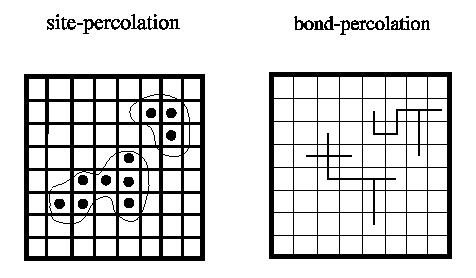
\includegraphics[scale=0.6]{Percolation1.jpg}
	\caption{Knoten- und Kantenperkolation}
\end{figure}
\vspace{0,5cm}
\\
Die einzelnen Plätze auf dem Quadratgitter werden zufällig jeweils mit einer Wahrscheinlichkeit $1-p$ geblockt. Es ist Konvention, die Wahrscheinlichkeit, dass ein Platz frei ist, mit $p$ zu bezeichnen, diese Konvention möchte ich hier erhalten. Geblockte Plätze können nicht besetzt werden. Man kann sich geblockte Plätze wie Wände eines Labyrinths vorstellen, durch die der Random-Walker später nicht hindurch kommt.  
\\
Nun definiert man einen Cluster als eine Gruppe benachbarter Quadrate, die begehbar sind, also nicht geblockt. Man nennt einen Cluster perkolierend, wenn sich der Cluster von einer Kante zur gegenüberliegenden Kante erstreckt, so dass zum Beispiel Wasser durch das Gitter fließen könnte, ähnlich wie es durch eine Kaffeemaschine (engl. 'percolator') perkoliert/sickert. Vereinfacht gesagt, kann ein Random-Walker auf dem perkolierenden Cluster sich unendlich ausbreiten und ist nicht 'eingesperrt'. Man kann sich nun leicht vorstellen, dass wenn kaum Felder geblockt sind (also $p$ nahe $1$) sich auf dem (unendlich großen) Quadratgitter stets ein perkolierender Cluster finden lässt, und wenn kaum Felder begehbar sind (also $p$ nahe $0$), sich nie ein perkolierender Cluster finden lässt. Es gibt dazwischen einen sogenannten 'kritischen Wert' $p=p_c \approx 0.5928$ \cite{Stauffer}, bis zu welchem das unendliche Quadratgitter perkoliert; auch Perkolationsschwelle oder englisch percolation-threshold genannt.
\noindent Historisch geht die Perkolationstheorie (engl. 'percolation theory') auf Paul Flory und Walter H. Stockmayer zurück, die sie während des zweiten Weltkriegs entwickelten, um Polymerisationsprozesse zu beschreiben. Der Polymerisationsprozess kommt durch das Aneinanderreihen von Molekülen zustande, die dadurch Makromoleküle bilden. Der Verbund solcher Makromoleküle führt zu einem Netzwerk von Verbindungen, die sich durch das ganze System ziehen können \cite{Wiki_Perkolationstheorie}.
\\
\noindent Üblicherweise wird der Beginn der Perkolationstheorie mit einer Publikation von Broadbent  und Hammersley aus dem Jahre 1957 in Verbindung gebracht, in welcher der Name eingeführt wurde und in welcher sie mit den oben erläuterten geometrischen und wahrscheinlichkeitstheoretischen Konzepten mathematischer behandelt wurde. Hammersley erwähnt in seiner persönlichen Geschichte der Perkolation in 'Percolation Structures and Processes', dass die (damals) neuen Computer, die für die Wissenschaftler dieser Zeit zugänglich wurden, einer der Gründe für die Entwicklung der Perkolationstheorie waren: Hier handelte es sich um Probleme, bei denen die Computer nützlich werden konnten.

\section{Perkolation auf dem Computer}
Es ist selbstverständlich nicht möglich, ein unendlich großes Quadratgitter mit zufällig geblockten und freien Gitterplätzen auf dem Computer zu erzeugen, daher wird hier stets ein endliches Quadratgitter (auf dem Computer in Form einer Matrix/Array gespeichert) und mit periodischen Randbedingungen ausgestattet. Um perkolierende Cluster dieser zufällig erzeugten Matrix zu finden, nutzt man den sogenannten Hoshen-Kopelmann-Algorithmus \cite{Fricke}.
Dieser Algorithmus lässt sich am besten an einem Beipiel erklären. Im nachfolgenden Bild sind freie Felder grau und geblockte Felder weiß. Graue Felder, die an einer Kante verbunden sind (wo der Random-Walker also von einem Feld ins andere kann), werden mit demselben Label versehen.
\begin{figure}[h!]
	\centering
	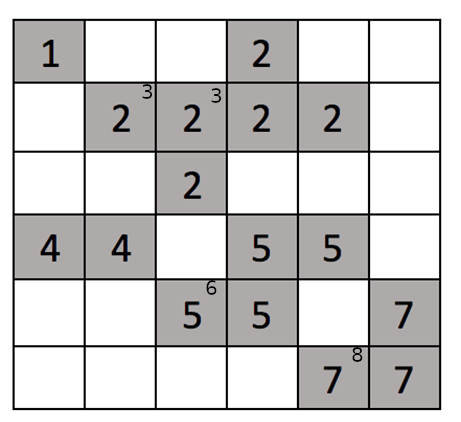
\includegraphics[scale=0.5]{H-K_algorithm.png}
	\caption{Veranschaulichung des Hoshen-Kopelmann-Algorithmus \break Die 'alten' Labels stehen -- falls unterschiedlich vom Label -- oben in der rechten Ecke.}
\end{figure}

\newpage
\subsection{Implementierung des Hoshen-Kopelmann-Algorithmus}
Die Idee, wie man dieses anschauliche Nummerieren auf den Computer überträgt, ist es die Matrix von zum Beispiel oben links beginnend abzugehen. Stößt man auf ein begehbares Feld (also einen Eintrag $1$ in der Matrix), vergleicht man das Label dieses Feldes mit den Labeln der Felder über und links von diesem Feld. Haben beide dasselbe Label, so wird dieses auch in das Feld, welches aktuell bearbeitet wird, eingetragen; haben die beiden Felder ein unterschiedliches Label, wird in einer Liste vermerkt man, dass diese beiden Label jetzt durch das aktuell zu bearbeitende Feld verbunden sind, und später zusammengefügt werden müssen. Sind die Felder oben und links von dem zu bearbeitenden Feld geblockt, labelt man das Feld mit dem nächst größeren, noch nicht benutzten Label. Ist man in diesem Verfahren die Matrix vollständig abgegangen, werden die verlinkten Labels zusammengefügt; es gilt als Konvention das kleinst mögliche Label zu verwenden. Zum Beispiel verlinkt das vierte Feld der zweiten Reihe in obiger Abbildung 2 die Labels 2 und 3 oder das vierte Feld der fünften Reihe die Labels 5 und 6.
\noindent In Python ist dieser Algorithmus für das Labeling (welcher auch in der Bildverarbeitung genutzt wird) bereits in der $scipy.ndimage$ Bibliothek als $measurements$ vorhanden. Nachfolgende Grafik zeigt einen Pseudocode\cite{Fricke} des Hoshen-Kopelmann-Algorithmus, man kann schön die Unterteilung in Scannen des Clusters, Verlinken von Labeln (union) und Finden der Equivalenzklasse (des Labels) (find) sehen.\newpage

\begin{figure}
	\centering
	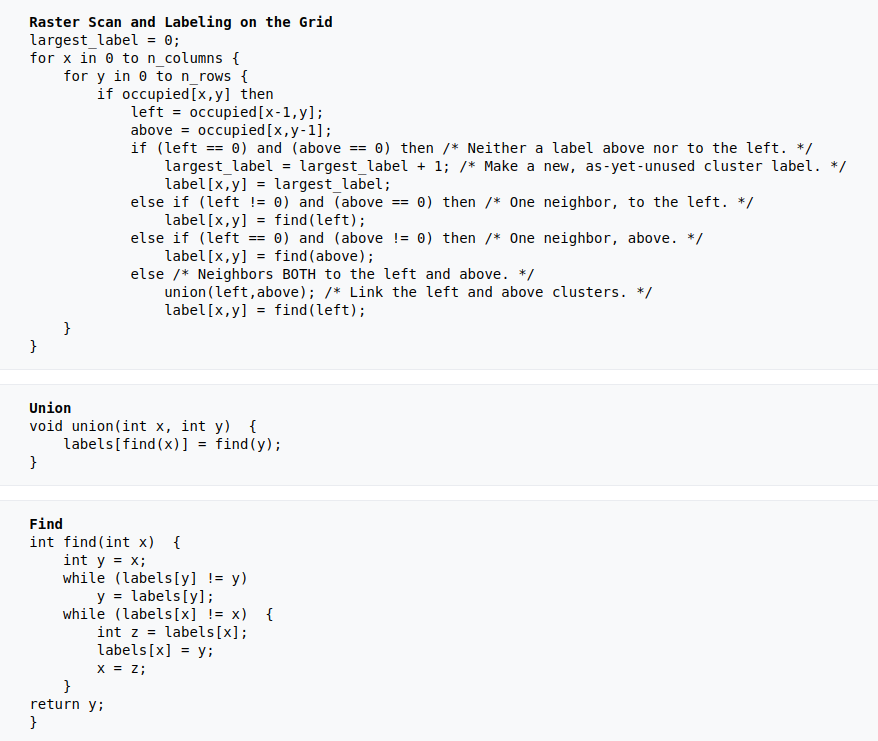
\includegraphics[scale=0.7]{HSK_pseudocode.png}
	\caption{Pseudocode des Hoshen-Kopelmann-Algorithmus}
\end{figure}

\clearpage
\subsection{Finden von gerichtet perkolierenden Clustern \label{gerichtet}}
Geht ein Cluster von einem Rand zum gegenüberliegenden Rand, also tritt an diesen beiden Kanten das selbe Label auf, so perkoliert dieser Cluster in der endlichen Matrix. Durch die periodischen Randbedingungen muss das Label am gegenüberliegenden Rand in der gleichen 'Höhe' auftreten. Es wird also einfach der linke Rand der Matrix abgegangen und das jeweilige Label mit dem Label an dem rechten Rand verglichen. Analog verfährt man mit dem oberen/unteren Rand. Diese Möglichkeit der Perkolation ist durch die periodischen Randbedingungen allerdings nicht die einzige, wie das nächste Unterunterkapitel zeigt.

\subsection{Diagonal perkolierende Cluster}
\begin{figure}[h!]
	\centering
	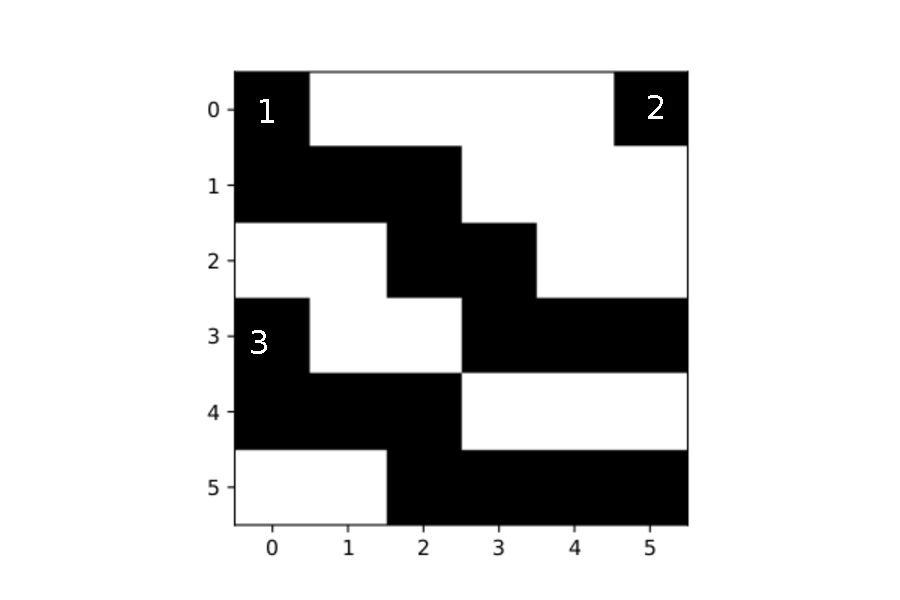
\includegraphics[scale=0.6]{diagonalperc1.pdf}
	\caption{Beispiel eines diagonal perkolierenden Clusters}
\end{figure}
\vspace{0,5cm}
\noindent Neben den in §\ref{gerichtet} beschriebenen gerichtet perkolierenden Clustern existieren noch Cluster, die diagonal über die periodischen Randbedingungen perkolieren. Ein Beispiel ist in Abbildung 4 zu sehen, aus dem ersten Cluster gelangt man über periodische Randbedingungen in den dritten Cluster, geht man aus der Position 5,5 nach unten, gelangt man in den dritten Cluster in der oberen rechten Ecke, mit einem Schritt nach rechts, ist man wieder in Cluster 1.
\\
\noindent Das Finden dieser Cluster stellt sich als schwieriger heraus, als das Finden der gerichtet perkolierenden Cluster, da man nicht einfach nur die Labels über die periodischen Randbedinungen verlinken darf, wie das nachfolgende Beispiel zeigt.
\begin{figure}[h!]
	\centering
	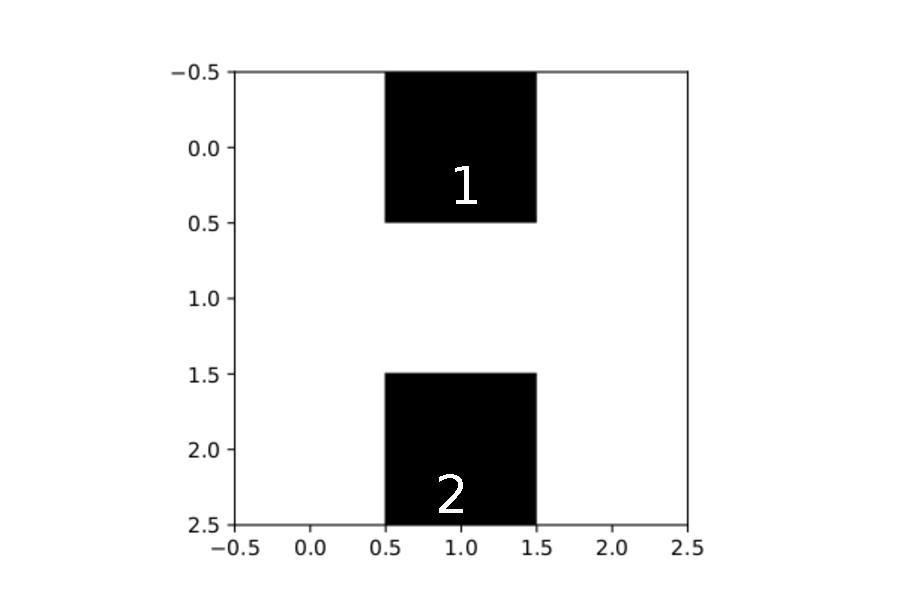
\includegraphics[scale=0.6]{noperc1.pdf}
	\caption{Es existiert offensichtlich kein perkolierender Cluster.}
\end{figure}

\vspace{0.5cm}
\noindent Würde man einfach das Labeln über periodische Randbedingung machen, würden beide Blöcke entsprechend Label 1 erhalten. Dem Kriterium aus §1.2.2 zufolge hätte man einen perkolierenden Cluster gefunden. Dies ist ganz offensichtlich falsch, da es sich um einen Cluster endlicher Größe handelt.
\\
\noindent Der (scheinbar) korrekte Algorithmus den perkolierenden Cluster zu finden, ist es, Cluster, die sich über periodische Randbedinungen berühren, in einer Verlinkungsliste zu speichern; zusätzlich zu den Labels muss die Richtung gespeichert werden. Man wählt die Konvention: links entspricht $(-1,0)$ rechts $(+1,0)$ unten $(0,-1)$ und oben entsprechend $(0,+1)$. Zu dem 'Weg' in der Verlinkungsliste muss die Summe der Richtungen gebildet werden, ist diese ungleich $(0,0)$, so perkolieren die Cluster, die verlinkt sind. Man muss (rekursiv) eine Suchfunktion implementieren, die alle zu einem gegebenen Label verlinkten Labels findet. Auf alle verlinkten Labels wird erneut rekursiv die Suchfunktion angewendet und so weiter. Wird das Ausgangslabel gefunden, müssen die Richtungen addiert werden und mit $(0,0)$ verglichen werden.
\\
\noindent Am Beispiel der in Abbildung 4 gezeigten Matrix bedeutet dies: $1 \rightarrow 3$ herhält Richtung $(+1,0)$, $3 \rightarrow 2$ erhält Richtung $(0,-1)$ und $2 \rightarrow 1$ wieder $(+1,0)$. Insgesamt hat dieser Weg also die Richtung $(+2,-1) \neq (0,0)$ und wird von dem Algorithmus gefunden.
\\
\noindent Im Gegensatz dazu, zeigt die nächste Abbildung eine Matrix mit einem $(0,0)$ Loop; man "läuft im Kreis" ohne dass wirklich eine Box durchschritten wird. Diese Matrix wird auch nicht als perkolierend gefunden, eignet sich aber sehr gut zum Debuggen.

\begin{figure}[H]
	\centering
	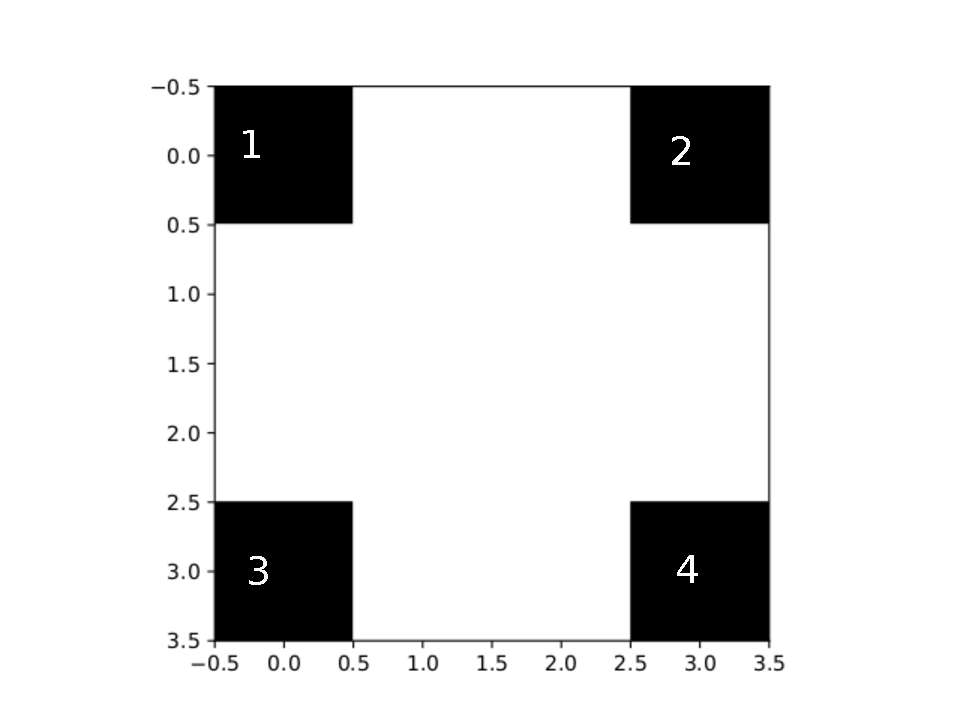
\includegraphics[scale=0.6]{noperc2.pdf}
	\caption{Es existiert offensichtlich kein perkolierender Cluster.}
\end{figure}

\clearpage

\noindent Das einzige Problem ist, dass dieser Algorithmus schlecht mit der Boxgröße skaliert, da die Anzahl der Labels quadratisch mit der Boxgröße wächst und die Zahl der Knoten nochmals quadratisch mit der der Labels zunimmt. Der Algorithmus skaliert also ungefähr mit $L^4$, wobei $L$ die Boxlänge bezeichnet. Unten sieht man den oben beschriebenen Teil zur Suche diagonal perkolierender Cluster als Python Code, welcher auch in den nachfolgenden Simulationen genutzt worden ist.


\begin{figure}[h!]
	\centering
	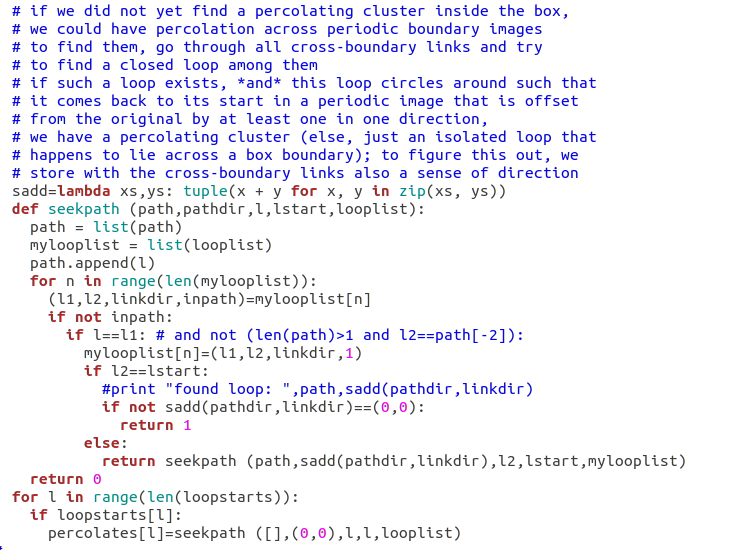
\includegraphics[scale=0.9]{diagcode.png}
	\caption{Python-Code zur Suche diagonal perkolierender Cluster}
\end{figure}

\clearpage


\section{Die fraktale Dimension des perkolierenden Clusters}
Fraktal ist ein vom Mathematiker Benoît Mandelbrot 1975 geprägter Begriff (lateinisch 'fractus' = 'gebrochen', von lateinisch 'frangere' = 'in Stücke zerbrechen'), der bestimmte natürliche oder künstliche Gebilde oder geo\-metrische Muster bezeichnet.
\\
\noindent Diese Gebilde oder Muster besitzen im Allgemeinen keine ganzzahlige Hausdorff-Dimension, sondern eine gebrochene -- daher der Name -- und weisen zudem einen hohen Grad von Skaleninvarianz bzw. Selbstähnlichkeit auf. Das ist beispielsweise der Fall, wenn ein Objekt aus mehreren verkleinerten Kopien seiner selbst besteht. Geometrische Objekte dieser Art unterscheiden sich in wesentlichen Aspekten von gewöhnlichen, glatten Figuren (zitiert aus: \cite{Fraktal_wiki}).
\\
\\
\noindent Perkolierende Cluster sind (unter Berücksichtigung der Gitterauflösung) ebenfalls fraktale Objekte. Ziel dieses Abschnitts ist es, die fraktale Dimension von perkolierenden Clustern zu bestimmen, um zu überprüfen ob meine Cluster dieselbe fraktale Dimension wie der Literaturwert haben. Ebenfalls soll die fraktale Dimension der perkolierenden Cluster mit der 'walk-dimension $d_w=1/\nu$' von Random-Walks auf ihnen verglichen werden. 
\\
Im folgenden Unterabschnitt wird eine (relativ simple) numerische Methode vorgestellt, mit welcher die fraktale Dimension des perkolierenden Clusters (und des Sierpinski-Dreiecks) bestimmt wird.
\subsection{Die Box-Counting-Methode}
Zur Bestimmung der fraktalen Dimension wird die sogenannte Box-Counting-Methode verwendet.\cite{Box_counting_wiki}
\\
\noindent Es werden sukzessive Boxen von der Größe $l=2^n$ , $l=2^{n-1}$ , ... , $l=2$ gebildet und jeweils die Anzahl der gesuchten Felder (hier also Labels des perkolierenden Clusters) gezählt. Die fraktale Dimension ist dann der Exponent, bzw. hier bei doppelt logarithmischer Auftragung der Vorfaktor, wie die Anzahl der gesuchten Felder und die Boxgröße miteinander skalieren. Hier wurde eine leichte Veränderung des Codes von Nicolas P. Rougier verwendet\cite{Rougier}. Rougier hat mit diesem Code erfolgreich die fraktale Dimension des Sierpinski-Dreiecks numerisch bestimmt.
\\
Genauere Details und mögliche Implementierung dieser Methode können dem nachfolgenden Python3 Code entnommen werden.
\\
\noindent Die Funktion $curve\_fit$ ist aus der $scipy.optimize$ Bibliothek.
\begin{figure}[H]
	\centering
	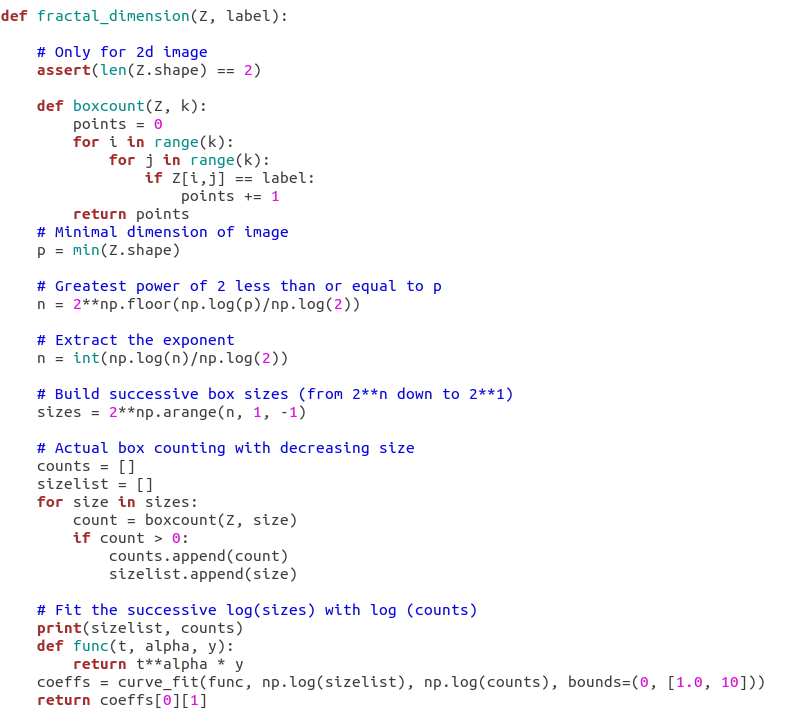
\includegraphics[scale=0.75]{fractaldim_code.png}
	\caption{Python3 Code für das Box-Counting zur Bestimmung der fraktalen Dimension des perkolierenden Clusters.}
\end{figure}

\newpage

\subsection{Ergebnisse der Box-Counting Analyse}
Die durchschnittliche fraktale Dimension eines perkolierenden Clusters, gemittelt aus 1000 perkolierenden Clustern, auf einem $1024\times 1024$ Gitter ($1024$ statt bisher $1000$ um eine Zweierpotenz mehr berücksichtigen zu können) bestimmt mit dem oben beschriebenen Python3 Code beträgt $d_f\approx 1.76$. Dies ist in guter Übereinstimmung mit zuvor getätigen Computersimulationen, die ebenfalls einen Wert zwischen $1.7 - 1.8$ für die fraktale Dimension $d_f$ vorhersagen (siehe \cite{Voss_1984}).
\\
\noindent Die nachfolgende Abbildung zeigt ein Histogramm mit der Bingröße $0.01$ zur Verteilung der mit der Box-Counting Analyse bestimmten fraktalen Dimension von $1000$ perkolierenden Clustern in einem $1024\times 1024$ Gitter.

\begin{figure}[H]
	\centering
	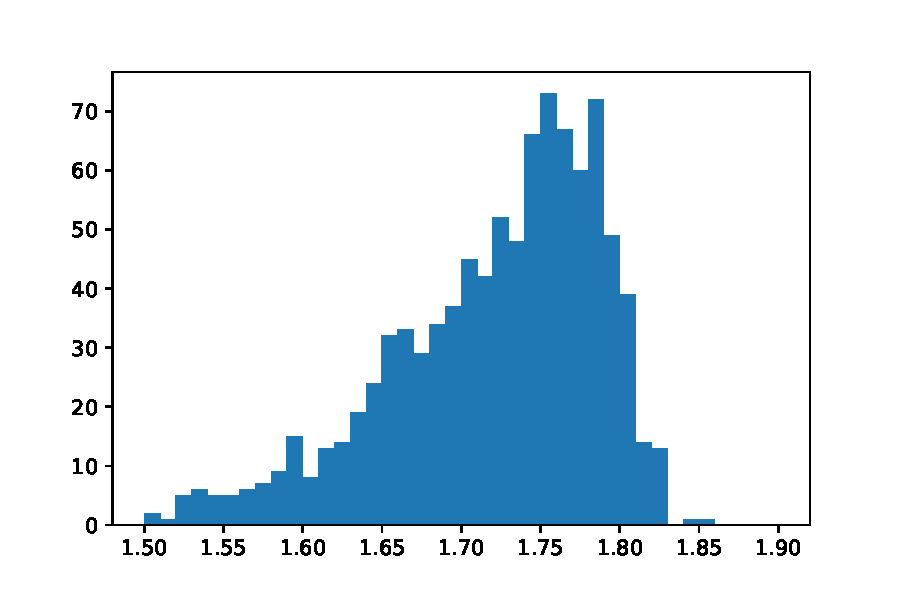
\includegraphics[scale=0.85]{fractal_histo.pdf}
	\caption{Histogramm der via Box-Counting Analyse bestimmten fraktalen Dimension von 1000 perkolierenden Clustern}
\end{figure}

\section{Random-Walk in ungeordneten Medien}

\subsection{"Normaler"\ Random-Walk}
Der (diskrete) Random-Walk auf dem freien Quadratgitter mit Hüpfwahrscheinlichkeit $\frac{1}{d}$ auf jeden der $d$ nächsten Nachbarn, wobei $d$ die Dimension des Gitter bezeichnet, unterliegt bekanntlich normaler Diffusion. Das heißt, dass das mittlere Verschiebungsquadrat (engl. mean squared displacement), welches im Weiteren mit $msd$ abgekürzt wird, linear mit der Anzahl an Schritten anwächst. Im kontinuierlichen Fall gilt die bekannte Formel:
\begin{align*}
msd(t)\equiv \langle \delta r^2 (t) \rangle =2dDt\ ,
\end{align*}
wobei (wie oben) $d$ die Dimension und $D$ der Diffusionskoeffizient sind, und hier gilt $D=\frac{1}{d}$.

\subsection{Random-Walk auf dem Perkolationsgitter}
Das Perkolationsgitter bei dem nur ein zufälliger Bruchteil der Gitterplätze begehbar sind und die anderen geblockt sind, ist ein besonders einfaches Modell für ein ungeordnetes Medium. Eine spannende Frage - die in den 70er und 80er Jahren des vergangenen Jahrhunderts durch eine Vielzahl von Computersimulationen geklärt wurde - ist, wie sich ein Random-Walker auf so einem unregelmäßigen Perkolationgitter für verschiedene $p$ ($=$ Wahrscheinlichkeit das ein Gitterplatz begehbar ist) verhält. Speziell geht man, motiviert durch die fraktale Struktur der Cluster, von einem Potenzgesetz:
\begin{align}\label{powerlaw}
msd(t) \sim t^{2 \nu},\ \ \nu=1/d_w
\end{align} 
aus, wobei $\nu$ als Diffusionsexponent bezeichnet wird und $d_w$ als 'walk dimension'. Der im Feld der weichen Materie bekannte französische Physiker Pierre-Gilles de Gennes nannte diese Fragestellung 1976 die 'Ameise im Labyrinth'.\cite{Stauffer} 
\\ 
\noindent Zuerst muss man die Hüpfwahrscheinlichkeiten festlegen, also ob $\frac{1}{f.n.N.}$ ($f.n.N.$ für freie nächste Nachbarn) oder wie bei dem freien Random-Walk $\frac{1}{d}$ und Züge auf ein geblocktes Feld ablehnen/verweigern. Für lange Zeiten sind beide Varianten äquivalent ('blind' vs 'myopic' ants)\cite{Havlin}.
\\
Nun überlegt man sich leicht die beiden Extremfälle $p$ nahe $1$ und $p$ nahe $0$. Im ersten Fall ($p \approx 1$) erwartet man sofort $\nu \rightarrow1/2$, da es kaum 'Hindernisse' gibt und der Random-Walker nahezu ungestört laufen kann. Andersherum, bei $p$ nahe $0$ erwartet man, dass es keine perkolierenden Cluster gibt, somit ist der Random-Walker 'eingesperrt' in sogenannte 'Taschen', damit das $msd$ beschränkt und somit $\nu \rightarrow 0$ für lange Zeiten. Besonders spannend ist dieses Problem also in der Nähe der Perkolationsschwelle $p=p_c$; hier findet sich ein nicht-trivialer Diffusionsexponent, d.h. ein Diffusionsexponent der weder $1/2$ noch $0$ ist. Gefen, Aharony und Alexander nannten diesen Effekt, dass das $msd$ weder normal (linear, $\nu = 1/2$) mit $t$ anwächst noch beschränkt ist, sondern für lange Zeiten asymptotisch einem Potenzgesetz mit $\nu \neq 1/2$ folgt, 'anomale Diffusion' \cite{PhysRevLett.50.77}. Diese anomale Diffusion wird, im Falle des unendlich großen Gitters, nur für $p=p_c$ gefunden, denn für $p<p_c$ existiert kein perkolierender Cluster, das $msd$ ist also beschränkt. Ist $p > p_c$ so gilt für $t \rightarrow \infty $ immer $msd \sim t$. Aber es gibt für $p$ nahe $p_c$ ein 'Fenster' mit $msd \sim t^{2\nu}$, wobei $\nu < 1/2$ ist (siehe auch \cite{Kammerer_2008} für ein schematisches Bild mit 'Fenster').

\subsection{Chemische Distanz}
Prinzipiell muss man, um über $msd$s zu sprechen, zuerst eine Metrik festlegen, um Abstände zu messen. Meist wird (wie hier auch geschehen) ohne Erwähnung einfach die Euklidische Metrik genutzt. Im Fall von ungeordneten Medien und besonders von perkolierenden Clustern kann auch die sogenannte 'chemische Distanz/Metrik' genutzt werden, welche wie folgt definiert ist:
'Die chemische Distanz zwischen Gitterplatz $a$ und Gitterplatz $b$ bezeichnet die minimale Anzahl Schritte, um (auf erlaubtem Wege) von $a$ nach $b$ zu kommen.' 
\\
\noindent Diese chemische Distanz kann auf dem perkolierenden Cluster offenbar stark von der Euklidischen Distanz abweichen, da Hindernisse 'gerade' Wege blockieren können und 'Umwege' erfordern.
 

\subsection{'all-cluster-' und 'percolating-cluster average'}

Es gibt im Allgemeinen zwei Varianten, wie man $\nu_{pc}$ auffassen kann, man mittelt über zufällige Startpunkte auf dem zufällig geblockten Quadratgitter oder man mittelt über Startwerte, die nur auf dem perkolierenden Cluster liegen ('all-cluster average' und 'percolating-cluster average'). Es ist zu erwarten, dass der Exponent bei dem 'all-cluster average' unter dem Exponenten des 'percolating-cluster average' liegt, da beim 'all-cluster average' auch in sogenannten Taschen gestartet wird, in denen das $msd$ beschränkt ist. Die aktuell bekannten 'Literaturwerte' sind $d_w^{a.c.} \approx 3.036$ und $d_w^{p.c.} \approx 2.878$, woraus sich $\nu_{pc}^{a.c.} \approx 0.329$ und $\nu_{pc}^{p.c.} \approx 0.347$ ergeben\cite{GRASSBERGER1999251}. In dieser Arbeit wurde versucht diese Werte durch Monte-Carlo-Simulation (MC) zu reproduzieren. Es wurde eine Gitterlänge $L=1000$ verwendet und die Perkolationsschwelle als $p_c = 0.592\ 746$ angenommen. Es wurden zu beiden Mittelungsvarianten über $100$ Läufe auf je $100$ zufälligen Matrizen gemittelt, wobei nicht auf diagonale Perkolation getestet worden ist (aus Laufzeitgründen). Die Läufe waren je $10^6$ MC-Schritte lang und wurden auf einem ($10$er-) logarithmischen Grid gespeichert mit 48 Speicherstellen. 
\begin{figure}[h!]
	\centering
	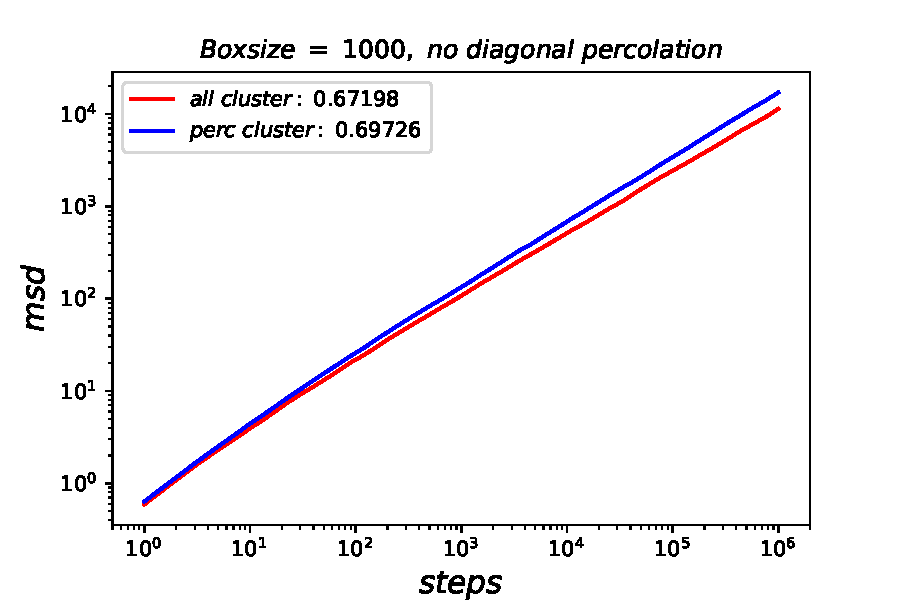
\includegraphics[scale=0.9]{acpcold1000.pdf}
	\caption{Ergebnisse meiner Python3 MC-Simulation \break Der 'all-cluster average' ist in rot, der 'percolating-cluster average' in blau; es wurden keine diagonal perkolierenden Cluster in die Statistik aufgenommen.}
\end{figure}
\vspace{0,5cm}
\newpage
\noindent Die Exponenten wurden über einen $scipy.optimize.curve\_fit$ als $2\nu_{pc}^{a.c.} \approx 0.6712$ und $2\nu_{pc}^{a.c.} \approx0.6973$ bestimmt. Die Methode, den Exponenten durch einen fit zu bestimmen, hat sich als (teilweise je nach Sampleanzahl deutlich) stabiler herausgestellt als das Bestimmen der Ableitung durch eine 'central-difference' oder 'forward-difference' Methode, welche unter sehr hohen numerischen Fehler leidet, da zwei sehr große Zahlen voneinander abgezogen werden, deren Differenz klein ist. Dieses Problem ist bekannt als 'catastrophic cancellation'. Nimmt man Werte, die weiter auseinander liegen (also ein größeres $h$), so wird die Ableitung ebenfalls sehr ungenau, da der Fehler quadratisch ('central-difference') beziehungsweise linear ('forward-difference') mit dem Abstand $h$ wächst. Ein lokaler Mittelwert hilft etwas,
die 'Zacken' in der numerischen Ableitung zu glätten, ist aber durch das logarithmische Grid mit Vorsicht zu genießen, da spätere Zeiten stärker gewichtet werden. Im nachfolgenden Plot ist die numerische Ableitung mit dem Fit-Parameter verglichen und ebenfalls die gefittete Kurve (in schwarz) an das 'all-cluster' mean-squared-displacement angelegt. Man erkennt, dass die numerische Ableitung, welche mit der 'forward-difference' Methode bestimmt wurde, und Fit übereinstimmen. Auf oben beschriebenes Glätten der Ableitung wurde verzichtet, da eine ausreichende Anzahl an Samples für eine relativ glatte Kurve vorliegt (soweit mean bei der Ableitung von stochastischen Daten von glatt reden kann). 
\\
\noindent Den Diffusionsexponenten kann man unter der Annahme einer 'power-law' für das $msd$, also Gleichung \ref{powerlaw} über die Formel:
\begin{align}\label{diffusionexponent}
	2\nu = \frac{msd'(t)}{msd(t)} \cdot t
\end{align}
bestimmen. Da $msd'(t) \sim 2\nu \cdot t^{2\nu -1}$ gilt, wobei sich der Proportionaltätsfaktor aufgrund der Linearität der Ableitung mit dem $msd$ im Nenner kürzt.
\begin{figure}[h!]
	\centering
	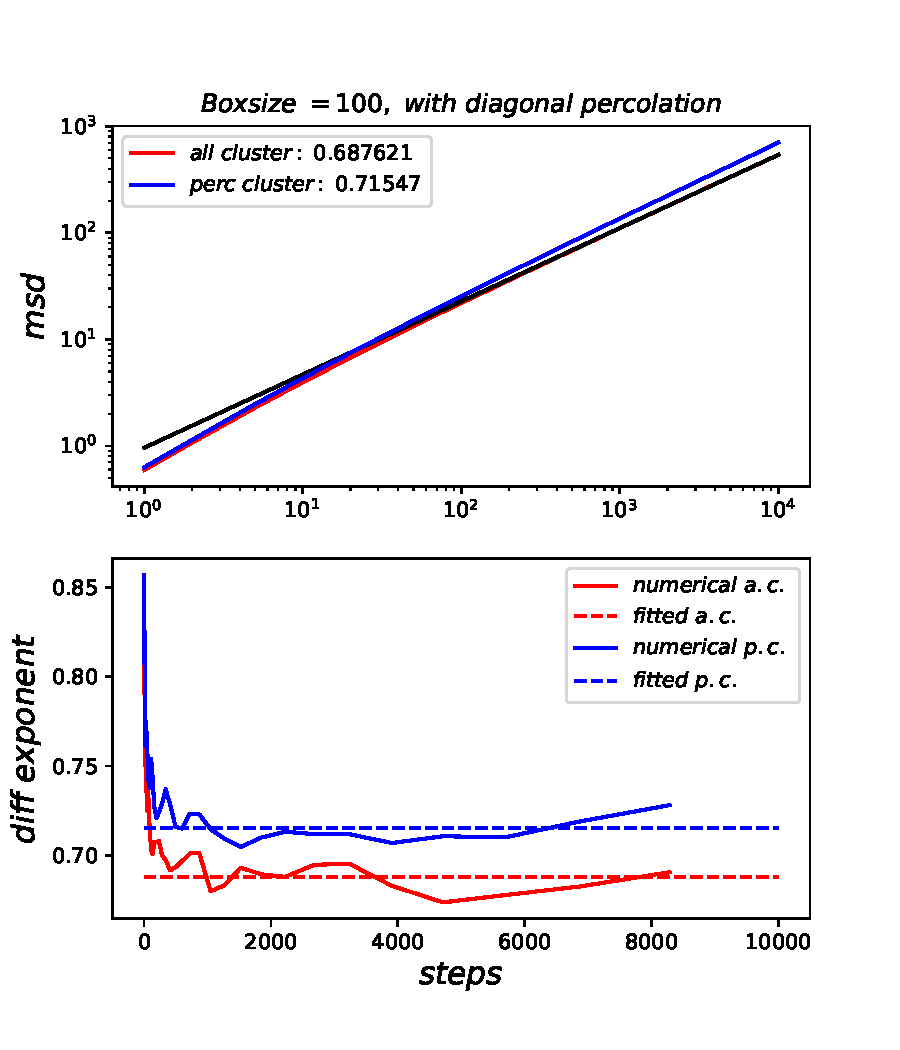
\includegraphics[scale=0.9]{newacpc100.pdf}
	\caption{Ergebnisse meiner Python3 MC-Simulation \break Der 'all-cluster average' ist in rot, der 'percolating-cluster average' in blau, es wurden keine diagonal perkolierenden Cluster in die Statistik aufgenommen.}
\end{figure}
\newpage


\subsection{Vergleich der Statistik mit und ohne diagonale Perkolation}
\noindent In kleineren Simulationsboxen treten finite-size Effekte auf. Die Diffusionsexponenten sind weiter von den Literaturwerten für eine unendliche Box entfernt; dennoch sind (bei gleicher Boxgröße), wie nachfolgender Plot zeigt, die Exponenten mit diagonal perkolierenden Clustern näher am Literaturwerten für eine unendliche Box. Es sind bei einer Boxgröße $L=100$ ca. $18,6\%$ der perkolierenden Cluster diagonal perkolierend. Größere Boxen sind aktuell durch zu hohe Laufzeit des Clustersuch-Algorithmus nicht (im Rahmen einer Masterarbeit, bzw. deren Einarbeitung) realisierbar.
\begin{figure}[h!]
	\centering
	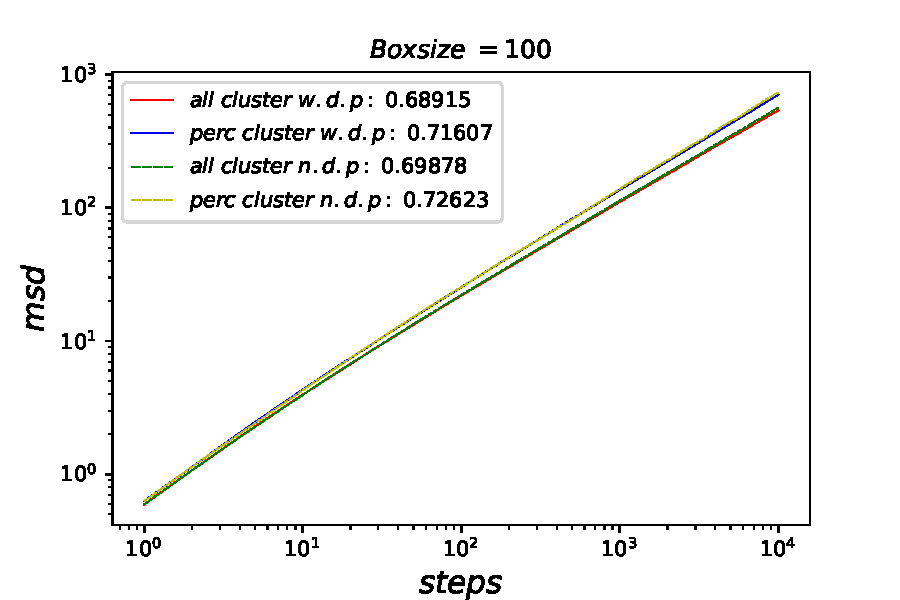
\includegraphics[scale=0.9]{both100.pdf}
	\caption{Vergleich von Statistik mit (w.d.p.) und ohne (n.d.p.) diagonal perkolierende Cluster, gesamplet über 1000 Läufe auf je 500 Matrizen.}
\end{figure}

\noindent Man sieht vor allem an den Werten, dass der Literaturwert von $2\nu_{pc}^{p.c.} \approx 0.694$ nun unterschätzt wird (bezogen auf den 'percolating-cluster average'). Zudem ist der Wert bei der Box mit Länge $L=1000$ ohne diagonal perkolierende Cluster näher am Literaturwert. Man sollte also lieber auf das Finden der diagonal perkolierenden Cluster verzichten und größere Boxen wählen, denn der 'finite-size' Fehler scheint größer als der Fehler, den das Auslassen der diagonal perkolierenden Cluster verursacht.
\subsection{Random-Walk auf diagonal perkolierenden Clustern}
Um den Einfluss der diagonal perkolierenden Cluster besser zu verstehen, habe ich eine Simulation von 1000 Läufen auf je 500 diagonal perkolierenden Clustern angefertigt ('percolating-cluster average'). Die Boxgröße beträgt $L=100$. Es wurde $\nu_{pc}^{p.c.} \approx 0.681$ gefunden, dieser Wert unterschreitet den Literaturwert von $\nu_{pc}^{p.c.} \approx 0.694$. Dies ist leicht einzusehen, denn diagonale Läufe haben ein geringeres $msd$, da ein Schritt nach (z.B.) rechts gefolgt von einem Schritt nach (z.B.) oben ein $msd$ von $2$ ergibt, wohingegen zwei Schritte in eine Richtung ein $msd$ von $4$ ergeben. Die diagonal perkolierenden Cluster führen also auch dazu, dass das $msd$ geringer wird. So lässt sich erklären, dass auch bei der Simulation der $L=1000$ Box in §2.4.4 beide Exponenten überschätzt werden.

\begin{figure}[h!]
	\centering
	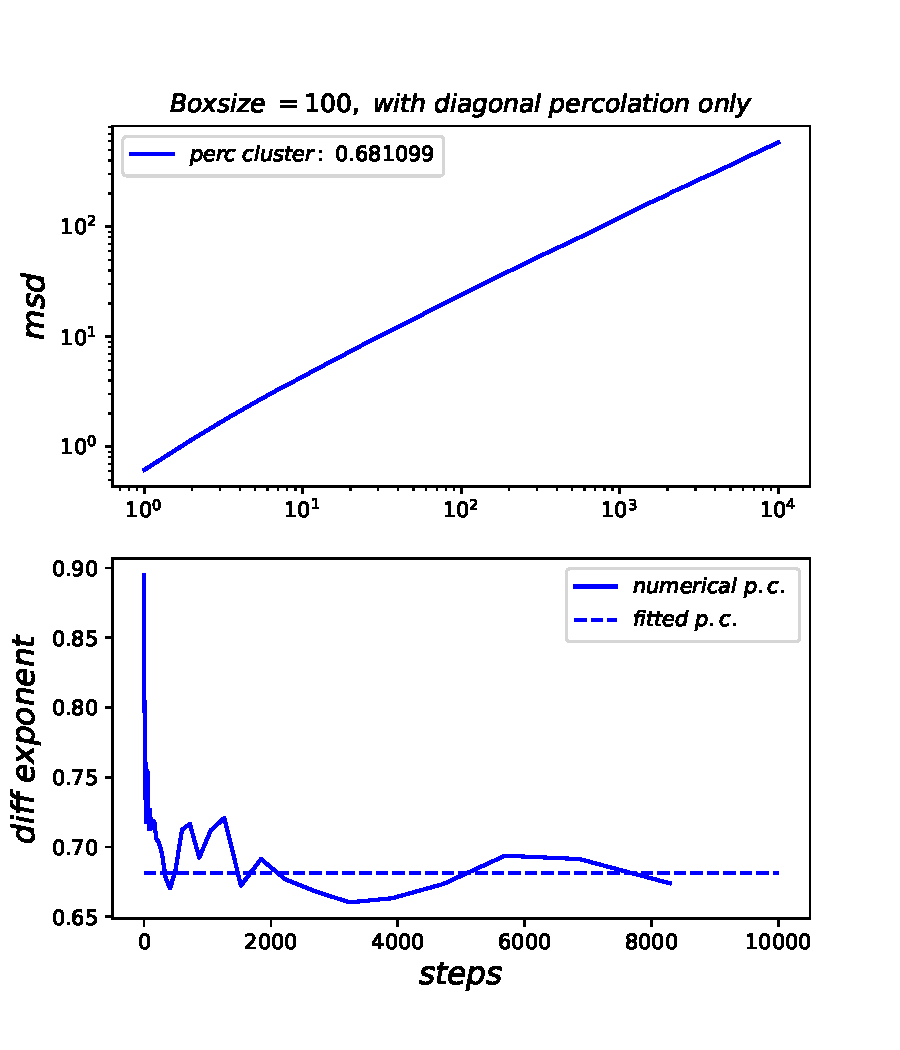
\includegraphics[scale=0.9]{diagpc100.pdf}
	\caption{Vergleich von Statistik mit und ohne diagonal perkolierende Cluster, gesamplet über 1000 Läufe auf je 500 Matrizen.}
\end{figure}


\newpage
\section{Spezielle Random-Walk Varianten auf dem Perkolationsgitter}


\subsection{Self-Avoiding Walk auf dem Perkolationsgitter}
Self-Avoiding Walks (kurz: SAW), also Random-Walks, die niemals zu einem zuvor besuchten Gitterplatz zurückkehren, sind ein Standardthema in der Physik der weichen Materie, da sie ein Modell für Polymerketten geben und meist auch eines der ersten Beispiele für einen nicht-markovschen stochastischen Prozess. Der Exponent $\nu^{SAW}$ des $msd$ beim SAW ist daher von besonderem Interesse, da er eine Verbingung zwischen mittlerer Größe eines Polymers und der Anzahl der Kettenglieder schafft:
\begin{align*}
\tilde R \equiv \sqrt{\langle R^2 \rangle} \sim N^{\nu^{SAW}},
\end{align*} 
wobei $\tilde R$ der Durchmesser des Polymers ist.
\\
Nun lässt sich auch leicht die Frage formulieren wie sich ein SAW auf dem Perkolationsgitter ausbreitet. Der normale Random-Walk ist langsamer geworden, genauer: $\nu_{pc} \equiv \nu_{pc}^{p.c.} < 1/2$, im Gegensatz dazu wird der SAW auf dem Perkolationsgitter schneller. In anderen Computersimulationen wurde $\nu^{pcSAW} \approx 0.78$ gefunden, wohingegen $\nu^{SAW}=3/4=0.75$ ist\footnote[5]{V. Blavatska und W. Janke, Europhy. Lett. 82, 6606 (2008)}$^,$\footnote[6]{N. Fricke und W. Janke, Europhys. Lett. 99, 56005 (2012)}. Die Nachstehende Graphik zeigt, dass auch endliche SAW sich auf dem
Perkolationscluster schneller ausbreiten als auf dem freien Gitter\footnote[7]{Lee, Nakanishi und Kim, Phys. Rev. B 39, 13 (1989)} Der SAW ist ein wichtiger Vergleich zu dem 'aktiven' Random-Walk.
\begin{figure}[h!]
	\centering
	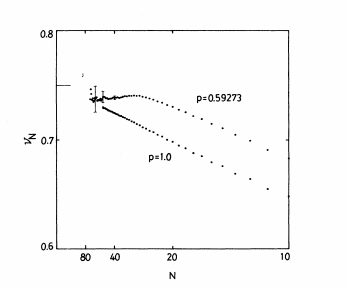
\includegraphics[scale=1.2]{saw.png}
	\caption{Ergebnisse einer MC-Simulation von Lee, Nakanishi und Kim \break $N$ bezeichnet die Länge des SAWs.}
\end{figure}

\clearpage

\subsection{'Aktiver' Random-Walk auf dem Perkolationsgitter}
Es wird nun eine Variante des Random-Walk betrachtet, welche zuvor noch nicht besuchte Plätze bevorzugt. Diese Variante eines Random-Walks kann man zum Beispiel für die Modellierung von Chemotaxis von Bakterien verwenden. Das Modell sieht wie folgt aus: Man generiert zuerst das Perkolationsgitter, danach werden begehbare Gitterplätze mit 'Nahrung' belegt, welche vom Random-Walker bei dem Besuch des jeweiligen Gitterplatzes vollständig 'gegessen' wird. Der Random-Walk erinnert also an 'PAC-MAN', der durch ein Labyrinth (den perkolierenden Cluster) nach Nahrung absucht.
\begin{figure}[h!]
	\centering
	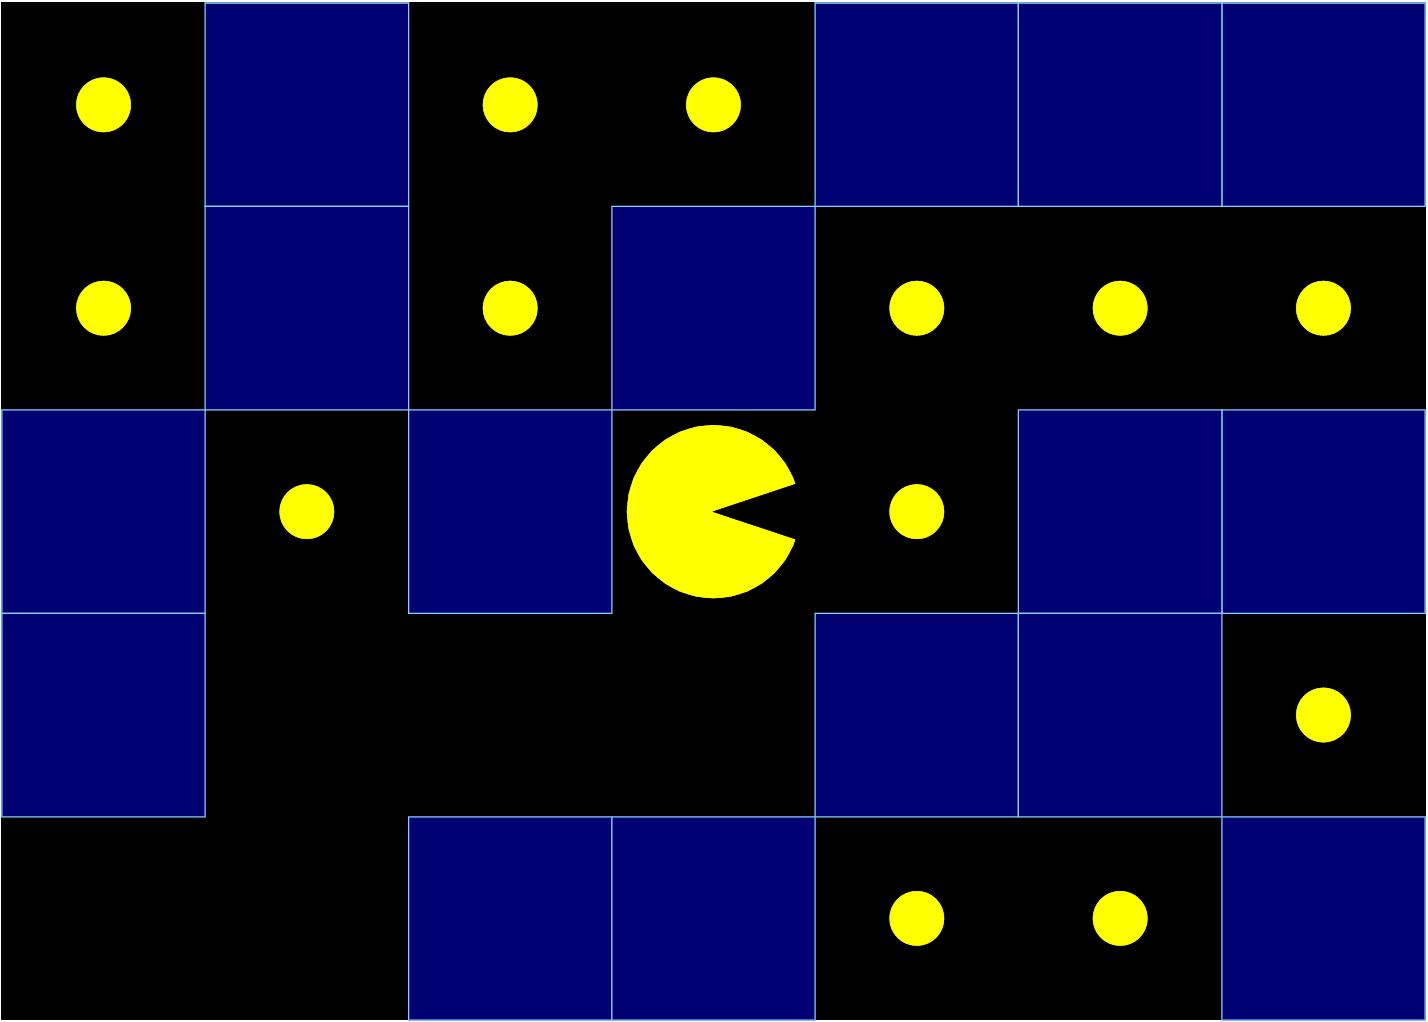
\includegraphics[scale=0.25]{pacman.png}
	\caption{Veranschaulichung des Modells \break Blaue Quadrate sind geblockte Gitterplätze, kleine gelbe Kreise sind Nahrung und 'Pacman' ist der Random-Walker\cite{doi:10.1063/1.4999485}.}
\end{figure}
\newpage


\noindent Die Wahrscheinlichkeiten für den nächsten Zug werden gemäß:
\begin{align}
p_{j \leftarrow i} = \frac{exp({F_j})}{\sum_j exp({F_j})}
\end{align}
berechnet, wobei $F_j$ die Menge der Nahrung an Gitterplatz $j$ ist, also $F$, falls Gitterplatz $j$ noch nicht besucht worden ist, und $0$, falls Gitterplatz $j$ zuvor bereits besucht wurde; $i$ ist dabei der Gitterplatz auf dem der Random-Walker aktuell ist. Dieses Modell scheint, insbesondere für $F \rightarrow \infty$, zuerst dem SAW sehr ähnlich zu sein, welcher auf dem Percolationsgitter schneller wird. Monte-Carlo-Simulationen dieses 'aktiven' Random-Walkers auf dem Perkolationsgitter zeigen, dass der Exponent kleiner ist, als der des normalen Random-Walkers auf dem Perkolationsgitter. Die nachstehende Abbildung zeigt Ergebnisse einer Monte-Carlo-Simulation mit je $100$ Walks auf $100$ Perkolationsgittern (Matrizen), wobei nicht auf diagonale Perkolation getestet worden ist, mit einer Größe von $1000 \times 1000$. Die Nahrung wird in meiner Simulation immer aus der Originalmatrix gelöscht und somit auch aus allen Kopien, welche durch die periodischen Randbedinungen entstehen. Diese Methode ist zwar nicht ganz korrekt (Quelle für finite-size-Effekte), führt aber zu keinem sichtbaren Fehler, solange die Wurzel aus dem $msd$ kleiner als die Boxgröße ist. Der Vorteil ist, dass diese Methode schneller ist und weniger Speicher benötigt. Die Perkolationsschwelle wurde wie zuvor als $p_c=0.592746$ angenommen.
\begin{figure}[h!]
	\centering
	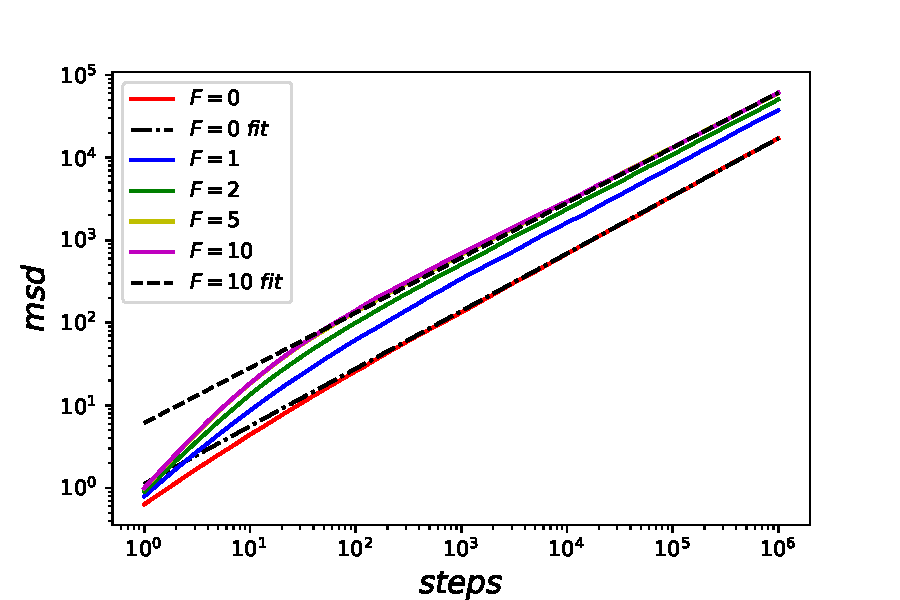
\includegraphics[scale=0.9]{food.pdf}
	\caption{Ergebnisse meiner Python3 MC-Simulation des 'aktiven' Random-Walkers auf perkolierendem Cluster ohne diagonale Perkolation \break Die gestrichelten Linien sind die mit scipy bestimmten Langzeit 'power-laws'.}
\end{figure}
\newpage

\noindent Es lässt sich erkennen, dass mit steigendem $F$ der Diffusionsexponent $\nu$, also die (halbe) Steigung der Kurve abnimmt entgegen der naiven Annahme, dass je größer $F$ ist, desto ähnlicher wird dieses Modell dem SAW.
Es wurden die folgenden Diffusionsexponenten gefunden:

\begin{tabular}[h]{l|c}
	F & $2\nu(F)$\\
	\hline
	0 & 0.697\\
	1 & 0.682\\
	2 & 0.664\\
	5 & 0.655\\
	10 & 0.666\\
\end{tabular}

\noindent Das gleiche Verhalten wurde auch bei einer kleineren Box von $L=100$ gefunden. Es wurde über 1000 Läufe auf je 100 Perkolationsgittern (inklusive diagonaler Perkolation) gemittelt.
\begin{figure}[h!]
	\centering
	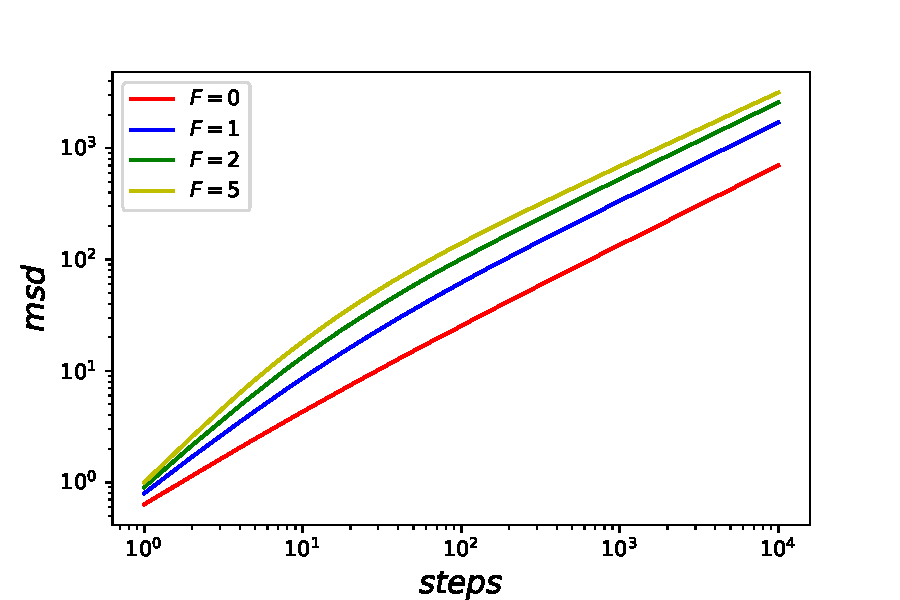
\includegraphics[scale=0.9]{newfood.pdf}
	\caption{Ergebnisse meiner Python3 MC-Simulation des 'aktiven' Random-Walkers auf perkolierendem Cluster mit diagonaler Perkolation}
\end{figure}
\newpage 
\noindent Erneut wurde die Nahrung die 'PAC-MAN gegessen hat', aus der originalen Matrix und somit auch aus allen Kopien, die durch die periodischen Randbedingungen entstehen, gelöscht. Die Wurzel aus dem $msd$ ist erneut kleiner als die Boxlänge $L=100$.\\
\noindent Dieses Modell zeigt auch sehr schön den Unterschied zwischen fraktaler und Random-Walk Dimension, da das Perkolationsgitter (also die fraktale Dimension $\approx 1.7\ -\ 1.8$) (siehe )\cite{Voss_1984}) unabhängig von $F$ ist, die Random-Walk Dimension (also $1/\nu$) aber nicht.
\newpage
\noindent Monte-Carlo-Simulationen mit einer Boxgröße von $L=25000$ und bis zu $10^6$ Walks auf bis zu $100\ 000$ Matrizen zeigen das gleiche Verhalten. In diesen Simulationen\cite{doi:10.1063/1.4999485} wurden die bereits besuchten Gitterplätze korrekt mit einem 'hash-table' nachgehalten. Die Ergebnisse dieser MC-Simulationen befinden sich in der nachfolgenden Abbildung.

\begin{figure}[h!]
	\centering
	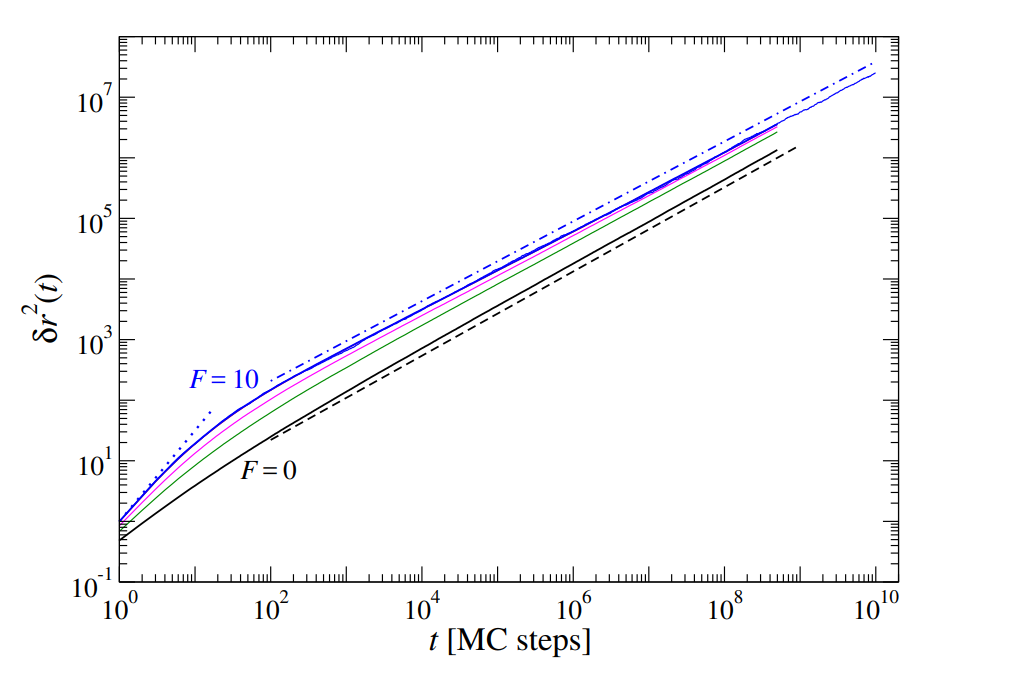
\includegraphics[scale=0.5]{food_thomas.png}
	\caption{Die blau gepunktete Linie zeigt die power-law des SAW ($\nu^{SAW}=3/4$), die blau gepunktet/gestrichelte Linie eine power-law zum Exponenten $\nu = 0.33$.\label{food_thomas}}
\end{figure}

\section{Zusammenfassung und Deutung: Aktiver Random-Walk auf perkolierendem Cluster}
Der aktive oder besser gesagt nahrungssuchende Random Walk auf dem perkolierenden Cluster scheint zunächst dem self-avoiding-walk auf perkolierendem Cluster zu ähneln, es stellt sich jedoch ein völlig verschiedenes Verhalten heraus. Der SAW breitet sich auf dem Perkolationsgitter schneller aus als ein normaler SAW auf dem freien Gitter. Der PAC-MAN-Walk wird langsamer als der klassische Random-Walk auf dem Perkolationsgitter und somit insbesondere viel langsamer als der, zunächst ähnlich erscheindene, SAW auf dem Perkolationsgitter.
\\
\noindent Wie lassen sich diese Unterschiede erklären?
\\
\noindent Dem neuen PAC-MAN-Walker sind sogenannte Sackgassen (dünne 'Äste' die keinen selbstmeidenden 'Rückweg' erlauben) des perkolierenden Clusters zugänglich, er wird sogar durch die Nahrung in diese Sackgassen gezogen und frisst sie leer. Anschließend muss der PAC-MAN-Walker diese Sackgassen diffusiv wieder verlassen, um den Cluster weiter nach Nahrung abzusuchen. Der SAW kann diese Sackgassen nicht betreten, verbringt also seine gesamte Zeit auf dem sogenannten 'backbone' des perkolierenden Clusters, auf welchen ich in dieser Arbeit nicht weiter eingehen werde (mehr dazu unter \cite{doi:10.1063/1.4999485} und \cite{PhysRevLett.101.125701}). 
\\
\noindent Der durch den PAC-MAN Prozess auftretende Exponent ist unterschiedlich zu bisher bekannten Exponenten von aktiver und passiver Mikroschwimmerdynamik und zudem abhängig von der 'Nahrungspropensität'.


\chapter{Eindimensionales Modell hungriger Walker}
In diesem Kapitel wird ein eindimensionales Modell simuliert um es mit semi-analytitischen Vorhersagen vergleichen zu können, da man in einer Dimension sich vieles deutlich leichter kombinatorisch errechnen kann.
\section{Mastergleichung für den 1D PAC-MAN}
Die Standardbehandlung von diskreten Markov-Prozessen ist das lösen einer sogenannten Mastergleichung, sie ist eine Art Bilanzierung des stochastischen Prozess.
\\
Grundsätzlich ist aufgrund der Nahrung der PAC-MAN Prozess nicht markov'sch, da die Übergangswahrscheinlichkeiten nicht nur von der Position abhängen sondern auch, wie der Walker dorthingelangt ist. Felder mit Nahrung werden gegenüber Feldern ohne mit dem Fakrot $e^F$ bevorzugt, somit sind die Übergangswahrscheinlichkeiten für einen Platz andere, wenn er zuvor zum Beispiel das Feld rechts von sich besucht hat, als wenn dieses Feld (rechts neben dem Walker) noch unbesucht ist.
\\
In diesem Kapitel wird aber eine sogenannte Markov'sche Einbettung für den Prozess mit Nahrung in 1D vorgestellt und anschließend eine Mastergleichung aufgestellt.
\\
Zunächst möchte ich kurz - aus der Vorlesung über stochastische Prozesse - wiederholen, was genau eine Mastergleichung ist.
\subsection{Mastergleichungen allgemein}
Unter einer Mastergleichung wird eine Differentialgleichung für die Wahrscheinlichkeit zu einer Zeit $t$ in einem Zustand $k$ zu sein bezeichnet.
\\
Es ergibt sich die folgende Gestalt für allgemeine Mastergleichungen:
\begin{align}
\partial_t p_k(t) = \sum_{l} \left[ W_{k \leftarrow l}p_l(t) - W_{l \leftarrow k}p_k(t)\right]\ ,
\end{align}
hierbei bezeichnet $p_k(t)$ die Wahrscheinlichkeit zur Zeit $t$ im Zustand $k$ sich zu befinden und $W_{l \leftarrow k}$ bezeichnet die Übergangsrate von Zustand $k$ nach Zustand $l$ (engl: 'hopping rates'). Man beachte, dass die Übergangsraten $W_{l \leftarrow k}$ nur von $k,l$ abhängig sind (nicht von der Historie), da es sich um einen Markov-Prozess handelt.
\\
Die vorderen Terme (mit dem $+$ Vorzeichen) auf der rechten Seite der Mastergleichung sind die sogenannten Gewinnterme, sie geben die Rate aus anderen Zuständen $l$ in den Zustand $k$ zukommen, gewichtet mit der Wahrscheinlichkeit $p_l$ im Zustand $l$ zu sein.
\\
Analog sind die hinteren Terme auf der rechten Seite der Mastergleichung die sogenannten Verlustterme ($-$ Vorzeichen), sie geben die Rate von Zustand $k$ in andere Zustände $l$, gewichtet mit der Wahrscheinlichkeit $p_k$ in Zustand $k$ zu sein, an.
\\
Es handelt sich somit um eine Bilanzgleichung für die Änderung der Wahrscheinlichkeit $p_k$.

\subsection{Markov'sche Einbettung und Mastergleichung eines 1D Walk mit Nahrung}
Allgemein ist es eine offene Frage der Theorie stochastischer Prozesse, ob jeder nicht Markov'sche Prozess in einen höherdimensionalen Markov-Prozess 'eingebettet' werden kann.
\\
Hier wird ein 1D Modell eines nicht Markov'schen Prozess vorgestellt, welcher sich sehr leicht in einen '2D' Markov-Prozess einbetten lässt vorgestellt.
\\
Man stelle sich einen hungrigen Walker (PAC-MAN) auf einem 1D Gitter vor, die Plätze rechts von ihm seien alle zu Beginn mit Nahrung belegt, die Plätze links von ihm seien alle frei. Die Übergangsraten sind somit $p_{\rightarrow} = \frac{e^F}{1+e^F}$ und $p_{\leftarrow} = \frac{1}{1+e^F}=:\varepsilon \in (0,\frac{1}{2}]$, falls der Gitterplatz rechts neben dem Walker noch Nahrung enthält (also nicht zuvor besucht worden ist). Ist der Gitterplatz rechts neben dem Walker zuvor besucht worden so sind die Wahrscheinlichkeiten nach rechts sowie nach links natürlich je $\frac{1}{2}$.
\\
Mit $p_i(t)$ sei die Wahrscheinlichkeit PAC-MAN an Gitterplatz $i$ zur Zeit $t>0$ zu finden bezeichnet. Die Anfangsbedinung (zur Startzeit $t=0$) sei fix durch $p_i(0) =\delta(i)$, und somit $p_i(t) \equiv p(i,t|0,0)$. Hier meint $p(i,t|i',t')$ die bedingte Wahrscheinlichkeit.
\\
Ohne Einschränkung der Allgemeinheit starte der Walker auf dem Gitterplatz $i=0$ und somit ist auf allen Gitterplätzen $>0$ zu Beginn Nahrung. Setzt man nun $r$ als den am weitesten rechts liegenden Gitterplatz der bereits besucht worden ist, so unterliegt das Tupel $(i,r)$ einem Markov-Prozess.
\\
Mit $p_{i,r}(t)$ sei bezeichnet, das der Walker zur Zeit $t$ sich an Gitterplatz $i$ befindet und zuvor bis einschließlich $r$ nach rechts gewesen ist. Offensichtlich gilt $r \geq i$ und damit  $p_{i,r}=0$  $\forall i>r$. Desweiteren gilt auch natürlich (durch unsere Wahl des Ursprungs) $p_{i,r}=0$ $\forall r<0$.
\\
In der Annahme eines kontinuierlichen Zeitlimes kann eine Mastergleichung für die drei Fälle $i=r$, $i=r-1$ und $i<r-1$ separat aufgestellt werden. Das Zeitargument wurde aus Gründen der Übersichtlichkeit fallen gelassen.
\\
Beginnen wir mit dem Fall $i=r$, hier ist klar, dass man mit Wahrscheinlichkeit $\frac{1}{2}$ von links aus der Position $i-1$ nach rechts springen kann, wenn man vorher den Platz $i$ bereits besucht hat, also aus dem Zustand $(i-1,r)$. Analog springt man mit Wahrscheinlichkeit $1-\varepsilon$ von $i-1$ nach $i$ wenn man diesen Platz vorher noch nicht besucht hat, also aus dem Zustand $(i-1,r-1)$. Gewinnterme on rechts also von $i+1$ kann es wegen $ r\geq i$ nicht geben. Die Verlustterme sind klar, der Walker kann mit Wahrscheinlichkeit $(1-\varepsilon)$ nach rechts springen, da er ja rechts neben sich auf keinen Fall schon war, oder mit Wahrscheinlichkeit $\varepsilon$ gegen die Nahrung nach links. Also ist $-p_{i,r}$ der Verlustterm.
\\
Nun zu $i=r-1$, der erste Gewinnterm ist offensichtlich der gleiche und der Verlustterm auch. Nur kann man nun, wegen $r=i+1$, nicht mehr nach rechts springen und dort noch neue Nahrung finden. Man kann nur von links gegen den Nahrungsbias springen, also von $(i+1,r)$ mit Wahrscheinlichkeit $\varepsilon$.
\\
Der Fall $i<r-1$ ist der klassische Random-Walk da $r\geq i+2$ also mindestens 2 Felder nach rechts keine Nahrung ist. 

\begin{align}\label{mastereq}
\partial_t p_{i,r}=
\begin{cases}
\frac{1}{2}p_{i-1,r} +(1-\varepsilon)p_{i-1,r-1}-p_{i,r}, & i=r
\\
\frac{1}{2}p_{i-1,r} +\varepsilon p_{i+1,r}-p_{i,r}, & i=r-1
\\
\frac{1}{2}p_{i-1,r} +\frac{1}{2} p_{i+1,r}-p_{i,r}, & i<r-1
\end{cases}
\end{align}
Wie man sieht hängen die Hüpfraten nicht von früheren Zuständen, sondern nur vom aktuellen Zustand $(i,r)$ ab.
\newpage
\noindent Analog für diskrete Zeitentwicklung (o.E mit $\Delta t=1$) stellt man die Übergangsgleichung
\begin{align}
p_{i,r}(t+1)=\sum_{i',r'}T_{i,r;i',r'}p_{i',r'}(t)\ ,
\end{align}
wobei $\underline{\underline{T}}$ die stochstische Übergangsmatrix mit Superindizes $(i,r)$ und $(i',r')$ ist. Aus der obigen Mastergleichung (\ref{mastereq}) kann man die Einträge von $\underline{\underline{T}}$ ablesen als:
\begin{align}
T_{i,r;i',r'}=
\begin{cases}
\frac{1}{2}\ , & i=i'+1 \land r=r' \land r \geq i
\\
1-\varepsilon\ , & i=i'+1 \land r=r'+1 \land r=i
\\
\frac{1}{2}\ , & i=i'-1 \land r=r' \land r > i+1
\\
\varepsilon\ , & i=i'-1 \land r=r' \land r = i+1
\end{cases}
\end{align}
wobei alle anderen Einträge null sind. ('Spaltensumme' $\sum_{i,r}T_{i,r;i',r'}=1$.)
\\
\\
Es ist die Wahrscheinlichkeit, den Walker an Gitterplatz $i$ zu finden die Summe über alle Wahrscheinlichkeiten der Zustände $(i,r)$, wobei wie immer $r\geq i$ gelten muss. Also
\begin{align}\label{(5)}
p_i = \sum_{r = i}^{\infty}p_{i,r}
\end{align}
Die linke Seite der Mastergleichung (\ref{mastereq}) lässt sich als
\begin{align}
\partial_t p_i=\partial_t p_{i,i} +\partial_t p_{i,i+1} +\partial_t \sum_{r=i+2}^{\infty} p_{i,r}
\end{align}
schreiben. Für jeden der drei Summanden setzten wir nun die passende rechte Seite aus der Mastergleichung (\ref{mastereq}) ein.
\begin{align}
\nonumber \partial_t p_i =&\ \frac{1}{2}p_{i-1,i} +(1-\varepsilon)p_{i-1,i-1}-p_{i,i}
\\
\nonumber &+\frac{1}{2}p_{i-1,i+1} +\varepsilon p_{i+1,i+1}-p_{i,i+1}
\\
\nonumber &+\frac{1}{2} \sum_{r=i+2}^{\infty}p_{i-1,r} + \frac{1}{2} \sum_{r=i+2}^{\infty}p_{i+1,r} - \sum_{r=i+2}^{\infty} p_{i,r}
\end{align}
Fassen wir nach (\ref{(5)}) zusammen so erhalten wir die folgende Mastergleichung:
\begin{align}\label{(6)}
\partial_t p_i = \frac{1}{2}p_{i-1}-p_{i}+\frac{1}{2}p_{i+1} + (\frac{1}{2}-\varepsilon)(p_{i-1,i-1} - p_{i+1,i+1})
\end{align}
Für $\varepsilon = \frac{1}{2}$ (also $F=0$) erhalten den klassischen 1D Random-Walk auf dem Gitter, wo wir $p_{i-1}-2p_{i}+p_{i+1}$ als 'finite difference' Approximation für die zweite partielle Ortsableitung auffassen können und somit im Kontinuumslimes die gewöhnliche Diffusionsgleichung mit der Diffusionskonstante $D=\frac{1}{2}$:
\begin{align}
\partial_t p = \frac{1}{2}\Delta p\ ,
\end{align}
wobei $\Delta:=\sum_{i=1}^{d}\partial_{x_i}$ der Laplace-Operator ist (in einer Dimension also \break $\Delta \equiv \partial_x^2$), erhalten.
\\
Ist hingegen $\varepsilon < \frac{1}{2}$ so verschwindet der hintere Term nicht. Wir setzen im Kontinuumslimes $p_{i,i} \rightarrow \hat{p}(x,t)$ und erhalten somit, über eine 'central difference' der ersten partiellen Orsableitung für $\hat{p}$ die folgende partielle Differentialgleichung:
\begin{align}
\partial_t p = \frac{1}{2} \partial_x^2 p -(1-2\varepsilon)\partial_x \hat{p}\ ,
\end{align}
wobei der Zusammenhang zwischen $p$ und $\hat{p}$ für $\varepsilon \in (0,\frac{1}{2})$ unklar ist.
Besonders im Fall $\varepsilon \rightarrow 0$ ist dieser offensichtliche Kontinuumslimes offenbar falsch, denn hier gilt $p_{i,r}=0\ \forall i \neq r$ und damit folgt $p=\hat{p}$. Dies führt zur 'advection-diffusion equation':
\begin{align}\label{advdiffeq}
\partial_t p = \frac{1}{2} \partial_x^2 p -\partial_x  p\ .
\end{align}
Diese wird mit einer um $\mu = t$ zentrierten Gaußkurve der Varianz $\sigma^2 = t$ gelöst.
\\
Für den Limes $\varepsilon \rightarrow 0$ müsste eine deterministische Transportgleichung:
\begin{align}\label{transporteq}
\partial_t p = -\partial_x p 
\end{align}
ohne Diffusionsterm folgen.
\\
Schauen wir uns also nocheinmal die Mastergleichung (\ref{mastereq}) an und setzen sofort $\varepsilon=0$ und $p_{i,r}=0\ \forall i \neq r$ ein. Es ergibt sich dann die korrekte Mastergleichung ($p_i \equiv p_{i,i}$):
\begin{align}
\partial_t p = p_{i-1}-p_i\ ,
\end{align}
welche in 'backward difference' genau die Transportgleichung (\ref{transporteq}) approximiert.
\\
Setzen wir auch umgekehrt in die 'advection-diffusion equation' (\ref{advdiffeq}) wieder sowohl für die erste sowie die zweite partielle Ortsableitung 'central difference' Approximationen ein, so wie wir auch ursprünglich vor der Identifikation $p=\hat{p}$ auf diese Gleichung gestoßen sind, so erhalten wir wieder:
\begin{align}
\partial_t p_i = \frac{1}{2}(p_{i+1}-2p_{i}+p_{i-1}) - \frac{1}{2}(p_{i+1} - p_{i-1})=p_{i-1}-p_i\ .
\end{align}
Ein ähnliches Problem, wo ungewollt ein Diffusionsterm auftritt ist die Lax-Stabilisation des 'FTCS'-Schemas (forward time centered space)\cite{Goetz}, auch Lax-Friedrichs-Schema genannt. 


\section{Kombinatorische Herangehensweise}
Es soll nun die Situation aus dem vorangegangen Abschnitt, dass ein Walker aus Gitterplatz $i=0$ startet und alle Gitterplätze rechts von dem Walker mit Nahrung belegt sind kombinatorisch untersucht werden. Erneut wird der am weitesten rechts liegende Gitterplatz ohne Nahrung mit $r$ benannt, sowie $\varepsilon:=\frac{1}{1+e^F}$ gesetzt.
\\
Schritte nach vorne ($i \rightarrow i+1$) zur Nahrung haben also die Wahrscheinlichkeit $(1-\varepsilon)$, Schritte nach hinten ($i \rightarrow i-1$) bei Nahrung auf Gitterplatz $i+1$ (oder anders ausgedrückt bei $r=i$) haben die Wahrscheinlichkeit $\varepsilon$. In der Situation, dass $r>i$ ist, gilt natürlich, dass die Wahrscheinlichkeit $1/2$ für beide Richtungen ist.
\\
Zum Zeitpunkt $t=2n$ möchte ich über Kombinatorik $p(x,t=2n|0,0)\equiv p(x,t=2n)$ bestimmen. Hierbei kann $x=2n-2m$ sein wobei $m$ die Schritte nach links ($i \rightarrow i-1$) zählt.
\\
Alle $2n$ Schritte mit der Nahrung (also nach rechts) zu gehen hat natürlich die Wahrscheinlichkeit:
\begin{align}
p(x=2n,t=2n) = (1-\varepsilon)^{2n}\ .
\end{align}
Nun zum nächste schwierigeren Fall, $x=2n-2$. Hier gibt es zwei Fälle, der letzte Schritt ist gegen den Nahrungs-bias nach hinten/links, ein Schritt mittendrin ist gegen den Nahrungs-bias gefolgt von einem Schritt nach vorne/rechts mit Wahrscheinlichkeit $1/2$. 'Mittendrin' sind genauer gesagt alle Schritte vor dem letzten Schritt. In dem einen Fall ist also ein Faktor $1/2$ und es ist $r=x$. Im anderen Fall sind keine 'freien Schritte' (also Faktoren $1/2$ dabei) und es ist $r>x$, dieser Anteil ist natürlich $(1-\varepsilon)^{2n-1}\varepsilon$. Nun zum $r=x$ Anteil, der 'backward-forward loop' hat die Wahrscheinlichkeit $\varepsilon \cdot \frac{1}{2}$, da der 'backward' Schritt gegen die Nahrung ist und der 'forward' Schritt ein freier Random-Walk Schritt ist. Dieser 'backward-forward loop' kann nun an einem aus $2n-1$ Schritten stattfinden, da er nur nicht als letzter Schritt stattfinden kann (dann ist nur noch ein Schritt, der 'loop' besteht aber aus zwei Schritten). Die Anzahl der Möglichkeiten diesen 'loop' zu platzieren ist also $2n-1$.
\\
Insgesamt also:
\begin{align}
p(x=2n-2,t=2n)=(1-\varepsilon)^{2n-1}\varepsilon+(2n-1)(1-\varepsilon)^{2n-2}\varepsilon\frac{1}{2},
\end{align}
man kann hier leicht checken, dass in beiden Fällen $2n$ Schritte gemacht werden.
\\
Ein weiterer netter Check ist $\varepsilon = 1/2$, hier muss sich eine Binomialverteilung also ${2n \choose 1} (1/2)^{2n}$ ergeben, was der Fall ist, da ${2n \choose 1}=2n$ ist.
\\
Diese Aufspaltung in Beiträge von $r=x$ und $r>x$ kann auch für den allgemeinen Fall $p(x=2n-2m,t=2n)$ verwendet werden, wobei $m \in \{1,2,...,n\}$ sein soll.

\subsection{Erster Fall, $r=x$}
Zuerst überlegen wir uns $r=x$, hier ist zunächst nur klar das der Faktor $1-\varepsilon$ natürlich insgesamt $2n-2m$ mal auftauchen sollte, da soweit die Nahrungsfront verschoben wird. Aus dieser Beobachtung ergibt sich, dass mindestens einmal gegen den 'food-bias' gegangen werden muss, da man ja sonst nach $x=2n$ laufen würde. Ebenfalls ist es leicht zu verstehen, dass man nicht mehr als $m$ mal gegen den 'food-bias' laufen kann, da man ja auch immer mindestens einen Random-Walk Schritt nach rechts/vorne braucht um wieder an die Nahrungsfront zu gelangen. Es kann also über einen Index $l$ summiert werden, welcher die Schritte gegen die Nahrung (und damit auch die 'freien Random-Walk' Schritte zurück an die Nahrungsfront) zählt. Bei $l$ $\varepsilon \frac{1}{2}$ Kombinationen verbleiben dann $2(m-l)$ Schritte für einen Random-Walk in der linken Halbebene, welcher eben genau beim letzten mal wieder an der Stelle ist wo dieser gestartet ist (die Anzahl dieser Walks ist gleich zu der die einen $2(m-l+1)$ Schritte Random-Walk in der positiven Halbebene machen). Die Anzahl dieser 'nicht-positiven' Random-Walks die nach $2(m-l)$ zurückkehren nenne ich $\hat{N}_{2(m-l)}$.
\\
Die $l$ Schritte gegen den 'food-bias' können an $2n-2m+1$ Stellen stattfinden ($x=0,1,...,2n-2m$), insbesondere mehrfach an der selben Stelle. Es handelt sich also um ziehen mit zurücklegen und ohne die Beachtung der Reihenfolge. Die Anzahl der Möglichkeiten beim Werfen von $k$ gleichen Würfeln mit N Flächen ist bekanntlich $N+k-1 \choose k$, in der Sprache der Urnenmodelle: Ziehen mit Zurücklegen, ohne Beachtung der Reihenfolge. In unserem Fall ergibt sich also der Vorfaktor $2n-2m+l \choose l$.
\\
Insgesamt ist damit die Wahrscheinlichkeit nach $t=2n$ Schritten an der Stelle $x=2n-2m$ unter der Bedingung $r=x$ zu sein:
\begin{align}
\nonumber p(x=2n-2m,t=2n|r=x) = (1-\varepsilon)^{2n-2m} \sum_{l=1}^{m}{2n-2m+l \choose l}\varepsilon^l \left(\frac{1}{2}\right)^l \cdot
\\
\cdot \sum_{\substack{k_1,...,k_l \\ k_1+k_2+\cdots k_l=m-l}} \left(\frac{1}{2}\right)^{2(m-l)} \hat{N}_{2k_1}\cdots \hat{N}_{2k_l}
\end{align}

\subsection{Positive Random-Walks}
Zuerst möchte ich das Reflexions oder Spiegelungsprinzip aus der Stochastik wiederholen.
\\
\\
\textbf{Reflexionsprinzip:}  Es seien $a,b \in \mathbb{N}$ und $i<j \in \mathbb{Z}$. Die Anzahl der Pfade von $(i,a)$ nach $(j,b)$, welche die x-Achse berühren, ist gleich der Anzahl der Pfade von $(i,-a)$ nach $(j,b)$

\begin{figure}[H]
	\centering
	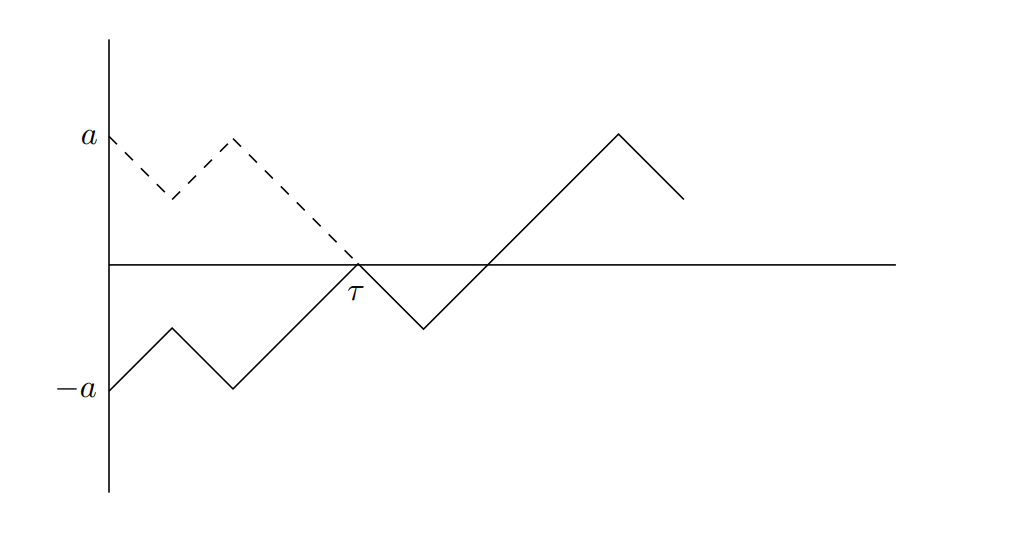
\includegraphics[scale=0.5]{spiegelungsprinzip.png}
	\caption{Veranschaulichung des Reflexions-/Spiegelungsprinzip.}
\end{figure}

\noindent Auf einen Beweis möchte ich an dieser Stelle verzichten und auf das Stochastik Skript von Herrn Prof. Löwe \cite{Stoch} verweisen, aus welchem auch die obige Abbildung entnommen ist.
\\
Nun ist $\hat{N}_{2p}$ gesucht, also die Anzahl aller Pfade von $(0,0)$ nach $(2p,0)$ welche nicht die negative Halbebene betreten (aber berühren der x-Achse ist erlaubt). Dies ist natürlich gleich der Anzahl der Pfade $(0,0)$ nach $(2(p+1),0)$ welche die x-Achse nicht berühren, was wiederum gleich der Anzahl der Pfade von $(1,1)$ nach $(2p+1,1)$, welche $y=1$ nicht unterschreiten. Diese Anzahl ist natürlich gleich der Anzahl aller Pfade von $(1,1)$ nach $(2p+1,1)$ minus der Anzahl an Pfade welche die x-Achse berühren. Die Anzahl der Pfade, die die x-Achse berühren ist nach dem Reflexionsprinzip gleich der Anzahl der Pfade von $(1,-1)$ nach $(2p+1,1)$, was genau $2p \choose p+1$ ist. Die Anzahl aller Pfade von $(1,1)$ nach $(2p+1,1)$ ist natürlich $2p \choose p$. Somit folgt:
\begin{align}
\hat{N}_{2p}={2p \choose p} - {2p \choose p+1}=\frac{1}{p+1}{2p \choose p}\ ,
\end{align}
da ${2p \choose p+1} = \frac{p}{p+1} {2p \choose p}$ gilt.
\subsection{Zweiter Fall $r>x$}

\section{Übergangsmatrixmethode für die Markov'sche Einbettung}
In diesem Abschnitt soll eine Möglichkeit vorgestellt werden, mit welcher unter zur Hilfenahme eines Computeralgebrasystems, wie zum Beispiel Mathematica oder der Sympy Erweiterung für Python, zu jedem Zeitpunkt $t$ die Wahrscheinlichkeit für einen Zustand $(i,r)$, wobei $i$ die Gitterposition und $r$ der am weitesten rechts liegende Gitterplatz ohne Nahrung ist, des zuvor vorgestellten Markov'schen Prozesses bestimmt werden kann.
\\
Erneut soll von $i=0$ aus gestartet werden und alle Gitterplätze zur rechten Seite seien initial mit Nahrung befüllt. Wie zuvor besprochen schaut die stochastische Übergangsmatrix $\underline{\underline{T}}$ wie folgt aus:
\begin{align}
T_{i,r;i',r'}=
\begin{cases}
\frac{1}{2}\ , & i=i'+1 \land r=r' \land r \geq i
\\
1-\varepsilon\ , & i=i'+1 \land r=r'+1 \land r=i
\\
\frac{1}{2}\ , & i=i'-1 \land r=r' \land r > i+1
\\
\varepsilon\ , & i=i'-1 \land r=r' \land r = i+1
\end{cases}
\end{align}

\noindent Es gilt $ \sum_{i,r} T_{i,r;i',r'}=1$, wobei die Summe natürlich auf Paare mit $r \geq i$ beschränkt ist, denn:
\begin{align}
\sum_{i,r} T_{i,r;i',r'}= \sum_{r\geq r'}T_{i'+1,r;i',r'} + T_{i'-1,r;i',r'}
\end{align}
jetzt gibt es zwei Fälle, erstens $i'=r'$ und zweitens $i'<r'$.
\\
In dem ersten Fall haben wir also die Möglichkeiten $r=r'$ woraus ein Schritt nach hinten folgt, also $T_{i'-1,r';i',r'}=\varepsilon$ und $r=r'+1$ woraus ein Schritt nach vorne folgt also $T_{i'+1,r'+1;i',r'}=1-\varepsilon$ in diesem Fall ist die Summe also $1$.
\\
Im Fall $i'<r'$ ist alles klar, denn dann ist es ein freier Random-Walk Schritt also $T_{i'\pm 1,r';i',r'}=1/2$.
\\
\\
Um die Wahrscheinlichkeiten nach $n$ Schritten zu haben müssen wir, mit dem Computeralgebrasystem, $\underline{\underline{T}}^n$ bilden und lesen de Wahrscheinlichkeiten aus den Einträgen $i,r;0,0$ ab, da unser Prozess bei $i'=r'=0$ starten soll.
\\
\\
Ein technisches Hindernis ist es, dass man vorher sich die maximale Schrittzahl vorgeben muss, denn die Größe der 4-dimensionalen Matrix beträgt die doppelte Schrittzahl hoch vier. Dies führt sehr schnell zu Speicherengpässen bei deutlich mehr als 20 Schritten. Eine Mathematica Implementation von Prof. Thomas Voigtmann befindet sich im Anhang an diese Arbeit.

\section{Definition der Schrittautokorrelationsfunktion}
Bei der Schrittautokorrelationsfunktion handelt es sich um die diskrete Version der bekannten Geschwindigkeitsautokorrelationsfunktion:
\begin{align}
g_{t_0}(\tau) = \langle \vec{v}(t_0+\tau) \cdot \vec{v}(t_0) \rangle\ .
\end{align}
Diese misst die Korrelation der Geschwindigkeit zum Zeitpunkt $t_0+\tau$ zur Geschwindigkeit zum Zeitpunkt $t_0$. Nun zur diskreten Version und ihrer Nützlichkeit.
\\
Durch die Nahrung wird der stochastische Prozess nicht-Markov'sch, d.h. das die Wahrscheinlichkeiten für den nächsten Zug nicht nur vom aktuellen Zustand (also der aktuellen Positionen der Walker) abhängig sind sondern auf von der Vergangenheit, also wie sie in ihre aktuellen Positionen gekommen sind. Um diese Äbhängigkeit zu vorherigen, und besonders zum ersten Schritt/Zug zu Untersuchen kann, in beliebiger Raumdmension, die folgende Korrelationsfunktion $g_{t_0}(\tau)$ gebildet werden. Es wird zuerst das (euklidische) Skalarprodukt zwischen dem Schrittvektor $\hat{e}(t_0)$ zur Zeit $t_0$ und dem Schrittvektor \break $\hat{e}(t_0+\tau)$ zur Zeit $t_0 + \tau$ eines Walkers berechnet und anschließend über alle Walker und alle Samples gemittelt, also bezeichnet $\langle \dots \rangle$ eine Ensemblemittelung. \\
\noindent Es ist demnach:
\begin{align}
g_{t_0}(\tau) = \langle \hat{e}(t_0+\tau) \cdot \hat{e}(t_0) \rangle\ .
\end{align}
Bei einem klassischen Random-Walk, unabhängigvon der Raumdimension, ist $g_{t_0}(\tau \neq 0)= 0$ für alle $t_0$ und natürlich gilt immer $g_{t_0}(\tau = 0)= 1$ denn $\hat{e}(t_0)$ ist einer der vier Einheitsvektoren $\pm \hat{e}_x,\ \pm \hat{e}_y$.
\\
\noindent Bei einem SAW in zwei Dimensionen ist $g_{0}(\tau = 1)= \frac{1}{3}$, denn nach dem ersten Schritt (dieser findet zur Zeit $t_0=0$ statt) gibt es drei Möglichkeiten: einmal in die gleiche Richtung, und zweimal senkrecht zum ersten Schritt. Jede der 3 Möglichkeiten wird zu $\frac{1}{3}$ angenommen, das Skalarprodukt istbei Schritt in die gleiche Richtung $+1$, senkrecht natürlich $0$, somit folgt $g_{0}(\tau = 1)= \frac{1}{3}$. Durch analoges Abzählen der Möglichkeiten und dem kombinatorischen Bestimmen der Wahrscheinlichkeiten findet man $g_{0}(\tau = 2)= \frac{1}{9}$ (weiterhin 2D SAW). Diese beiden Werte liefern einen Anhalt für die richtige Implementierung der Schrittautokorrelationsfunktion, denn die ersten drei Schritte des PAC-MAN-Walks in 2D ähneln (bei $F \geq 5$ zumindest) stark dem SAW. (Weitere 2D SAW Schritte sind schwer abzuzählen.)
\\ 
Offensichtlich ist $g_{t_0}(\tau)$ positiv wenn mehr Schritte zur Zeit $t_0+\tau$ in als entgegen der Richtung des Schrittes zur Zeit $t_0$ gegangen sind und negativ anders herum. 

\section{Mean-Squared-Displacement und Schrittautokorrelation für viele Walker}
Neben dem $msd$ kann erneut die Autokorrelation der Schritte $g_{t_0}(\tau)$ betrachtet werden. Aus dieser Größe kann man ablesen, wie stark der Schritt zur Zeit $t_0 + \tau$ mit dem Schritt zur Zeit $t_0$ korreliert ist.
Die Schrittautokorrelation eines einzigen Walkers auf einem vollem Nahrungsgitter, kann man, für große $F$ wie etwa $F=5$ und die ungefähr ersten 10 Schritte, sofort als 
\begin{align}
g_{0}(\tau) \approx \left(\frac{e^F}{e^F+1}\right)^{\tau}
\end{align}
abschätzen, da nach jedem Schritt die Wahrscheinlichkeit $\frac{e^F}{e^F+1}$ ist, das der nächste Schritt wieder in die selbe Richtung erfolgt. Diese Abschätzung vernachlässigt völlig den negativen Anteil, für den aber ein Schritt in die Gegenrichtung nötig ist, welcher für $F=5$ den Faktor $\frac{1}{e^5 + 1} < 0.007$ beinhaltet. Der erste Schritt ist $\tau = 0$ der zweite $\tau=1$, und so weiter. Die Startzeit $t_0$ möchte ich auf $t_0=0$ setzen.
\\
\noindent Auch für viele Walker lässt sich eine längere Korrelation zum ersten Schritt vermuten, da bis zum erreichen der Fressspur eines benachbarten Walkers die Schritte nahezu deterministisch in die Richtung des ersten Schrittes erfolgen.
\\
\noindent Ungefähr die Hälfte der Walker bewegt sich auf Walker vor sich zu, die andere Hälfte bewegt sich auseinander. Die Walker die sich aufeinander zu bewegen erreichen sich im Mittel nach etwa $\frac{1}{2 \rho}$ Schritten, wobei $\rho$ die Dichte der Walker ist.
\\
\noindent Die Schrittautokorrelationsfunktion sollte also nach $T = \frac{1}{2 \rho}$ Schritten nur halb so groß sein wie die des einzelnen Walkers nach der gleichen Anzahl Schritte. Bei 10\% Dichte also nach etwa 5 Schritten. Die Schrittautokorrelationsfunktion, eines einzigen hungrigen Walkers umgegeben von Nahrung, nach 5 Schritten ist $\left(\frac{e^F}{e^F+1}\right)^{4}$. Setzt man nun $F=5$ ein und rechnet das ganze aus so erhält man ungefahr $g_0(4) \approx 0.97$ (der 5te Schtritt findet zur Zeit $\tau =4$ statt). Nach obiger Überschlagsrechnung erwartet man also, dass die bei 10\% Walkerdichte simulierte Schrittautokorrelationsfunktion nach 5 Schritten knapp unter $0.5$ liegt.
\\
\noindent Zudem sollte bei 10\% Dichte nach ungefähr 10 oder 11 Schritten die Nahrung 'weggefressen' sein und die Schrittautokorrelationsfunktion ungefähr bei 0 ein. Beim einzelnen Walker hingegen sollte sie, nach 11 Schritten, bei $\left(\frac{e^F}{e^F+1}\right)^{10}\approx 0.935$ liegen.
\\
\\
\noindent In der nachfolgenden Grafik werden die Simulationsergebnisse gezeigt. Man sieht das die Schrittautokorrelationsfunktion tatsächlich, wie die oben Begründetet Vermutung sagt, nach 5 Schritten knapp unter $0.5$ ist. Die zweite 'Vermutung', dass nach etwa 11 Schritten die Schrittautokorrelationsfunktion auf 0 abgefallen ist, wird auch die die Simulation bestätigt.



\begin{figure}[H]
	\centering
	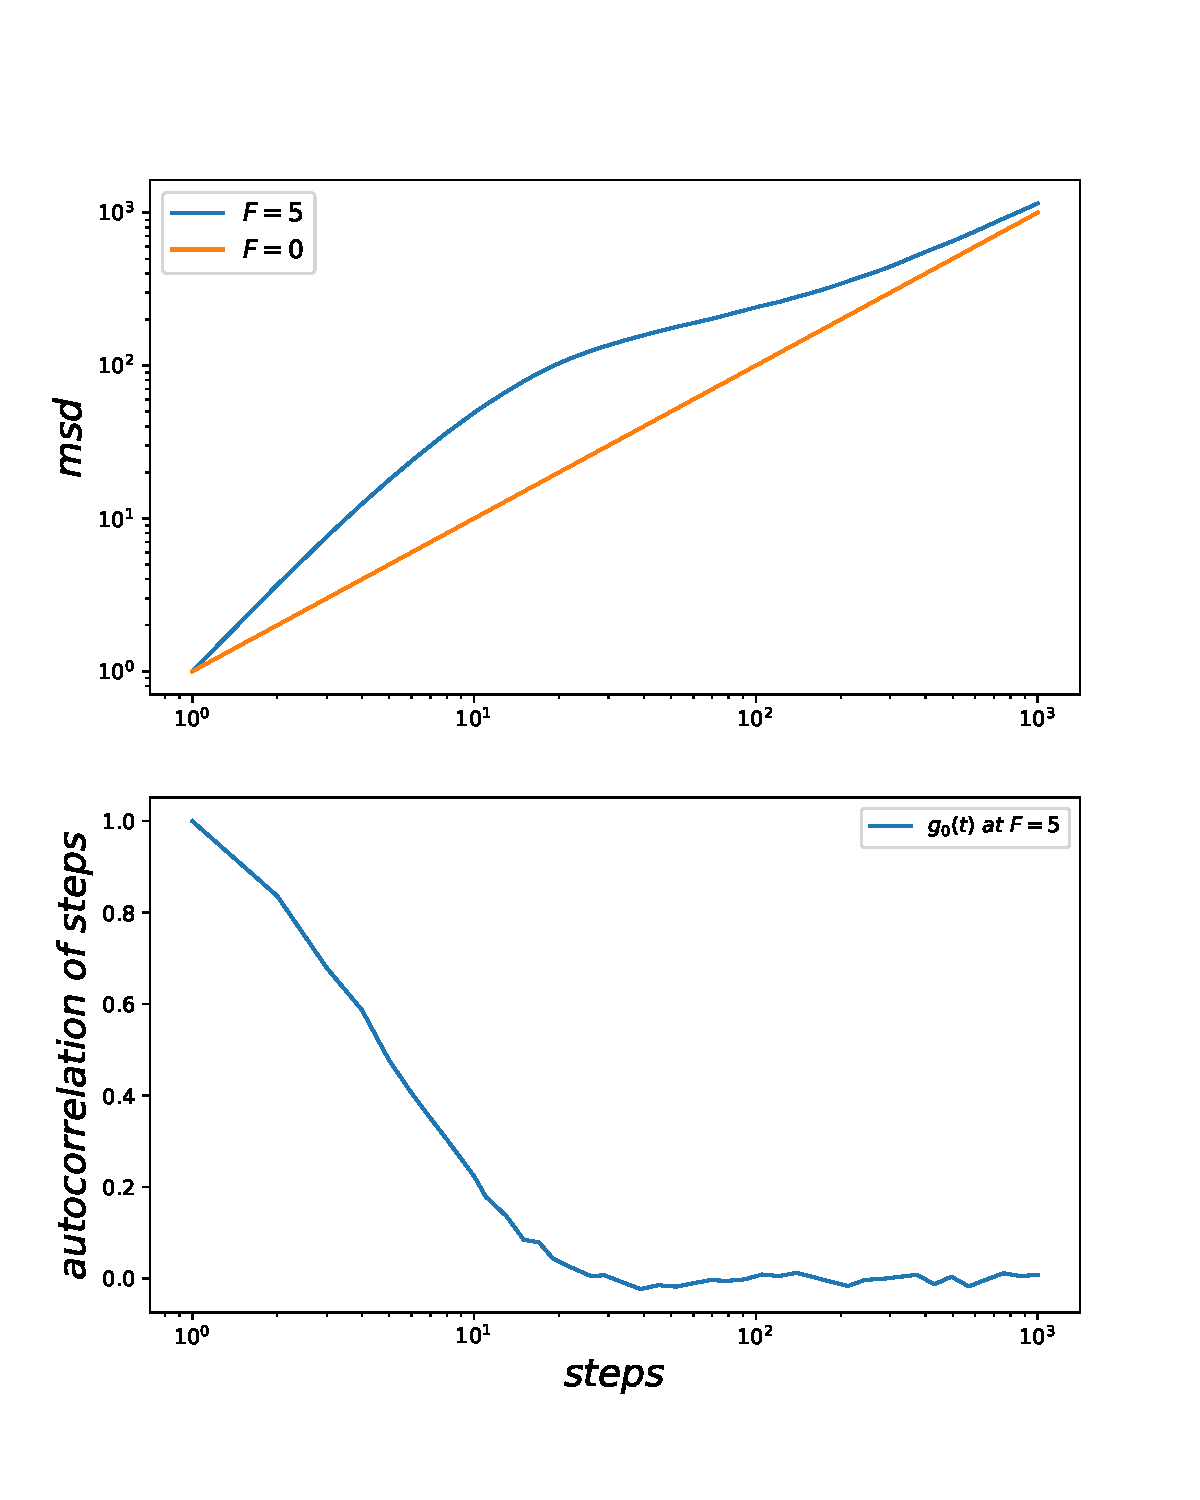
\includegraphics[scale=0.7]{onedescp.pdf}
	\caption{Autokorrelation der Schritte des eindimensionalen Modells. Es wurde über 100 Läufe, also $10^4$ Samples gemittelt.}
\end{figure}


\chapter{Viele Random-Walker auf dem freien Cluster mit Nahrung (2D)}
\section{Interaktion der Random-Walker}
Die einzelnen Random-Walker haben keine direkte Interaktion untereinander, es ist also insbesondere auch möglich, dass zwei (oder mehrere) Random-Walker auf der gleichen Position im Gitter sitzen. Der einzige Wechselwirkungseffekt der bei diesem Modell vorliegt ist, dass die Walker sich gegenseitig 'Nahrung wegessen' und somit die Umgebung eines anderen Walkers verändern und damit auch die Wahrscheinlichkeiten wohin der nächste Schritt ausgeführt wird. Man redet in so einem Modell also von einer durch 'Chemotaxis' induzierten Wechselwirkung. Es wurden zwei Zugversionen getestet, einmal ziehen alle Random-Walker zur selben Zeit und alternativ ziehen die Random-Walker sukzessive, also zuerst Random-Walker 1, gefolgt von Random-Walker 2 und so weiter. \\
\noindent Die Wahrscheinlichkeiten, wohin ein Random-Walker zieht werden wie in \cite{doi:10.1063/1.4999485} gemäß:
\begin{align}
p_{j \leftarrow i} = \frac{exp({F_j})}{\sum_j exp({F_j})}
\label{Wkeiten}
\end{align}
berechnet, wobei $F_j$ die Menge der Nahrung an Gitterplatz $j$ ist.

\section{Gleichzeitiges Ziehen\label{gleichzeitig}}
\subsection{Mean-Squared-Displacement}
In diesem Abschnitt werden Ergebnisse einer Monte-Carlo-Simulation von 1000 (also einer Dichte von 10\%, da $10^4$ Gitterplätze zur Verfügung stehen) hungrigen Walkern (PAC-MAN's) auf einem mit Nahrung bestückten $100 \times 100$-Gitter, mit periodischen Randbedingungen, vorgestellt. Die 'Nahrungspropensität' beträgt $F=5$ und es werden 100 Läufe simuliert um über insgesamt $10^5$ $msd$'s zu mitteln. Die Startpositionen der Walker werden unabhängig voneinander mit über dem gesamten Gitter gleichverteilter Wahrscheinlichkeit zufällig gewählt.

\begin{figure}[h!]
	\centering
	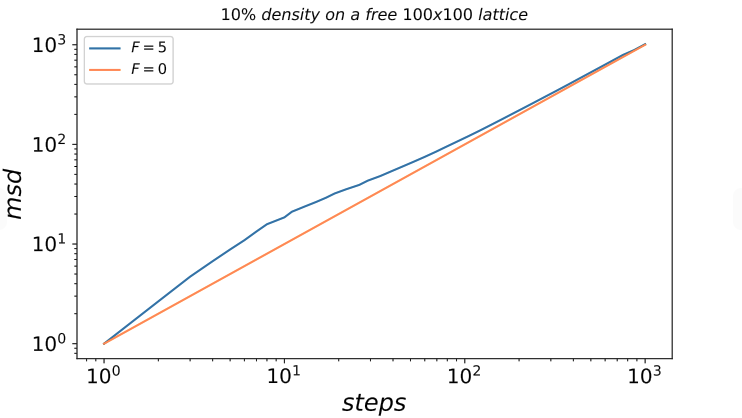
\includegraphics[scale=0.8]{msd10_1.png}
	\caption{$msd$ für 1000 PAC-MAN's auf $100\times 100$-Gitter mit Nahrung.}
\end{figure}

\noindent Es lässt sich auf den etwa ersten 10 Schritten ein superdiffusives Regime, also ein Bereich in dem der doppelte Diffusionsexponent $2\nu > 1$ ist, erkennen, dies ist nach der single-Walker-Dynamik zu erwarten, denn durch die Nahrung ergibt sich ein extrem starker 'bias' in Richtung zuvor unbesuchter Felder. Der Walk ähnelt daher auf den ersten Schritten dem SAW.
\\
\noindent Nach etwa 100 Schritten ist das $msd$ wieder in etwa diffusiv, jeder Walker hat einen Bereich von etwa $10\times 10$ Feldern 'abgefressen'. Interessant ist die Frage, ab wann ungefähr der Nahrungsverbrauch verschwunden ist? Würden die Walker nur auf zuvor unbesuchte Felder ziehen, so wäre nach dem 9ten oder 10ten Schritt keine Nahrung mehr vorhanden (je nach Startposition).
\\
\noindent Zwischen dem superdiffusiven Regime zu Beginn und der normalen (freien) Diffusion auf lange Zeiten liegt ein subdiffusives Regime, also ein Bereich in dem der doppelte Diffusionsexponent $2\nu < 1$ ist.

\subsection{Nahrungsvorrat und Diffusionsexponent}
Um mehr über den Prozess zu lernen, bietet es sich sofort an, die Entwicklung des Nahrungsvorrats gegen die Zeit (MC-Schritte) aufzutragen und mit dem Diffusionsexponenten zu vergleichen. In Gleichung \ref{diffusionexponent} wird erklärt wie man diesen mit Hilfe der (numerischen) Ableitung bestimmt. Aufgrund der geringen Samplezahlen muss hier eine lokale Glättung (ähnlich wie eine Ausgleichskurve) vorgenommen werden. Der Diffusionsexponent gibt Auskunft über das Regime, in dem sich der Prozess befindet, also zeigt dieser an, ab wo der Übergang von Superdiffusion auf Subdiffusion stattfindet.
\\
\noindent Die nachfolgende Abbildung \ref{food} zeigt, dass der subdiffusive Bereich kurz vor dem Verschwinden aller Nahrung beginnt, aber der Diffusionsexponent minimal ist, zu dem Zeitpunkt, wo genau die letzte Nahrung verschwunden ist. Ab diesem Moment liegt ein normaler Random-Walk vor, da die Teilchen keine Wechselwirkung mehr untereinander haben. Somit ist klar, das sich der (doppelte) Diffusionsexponent $2\nu$ wieder auf $1$ einstellen muss. Genau dies sieht man auch, nach ca 30 Schritten ,wo dann alle Nahrung 'gegessen' ist, steigt $2\nu$ wieder an, bis schließlich auf 1, was der freien Diffusion auf dem Quadratgitter entspricht.

\begin{figure}[H]
	\centering
	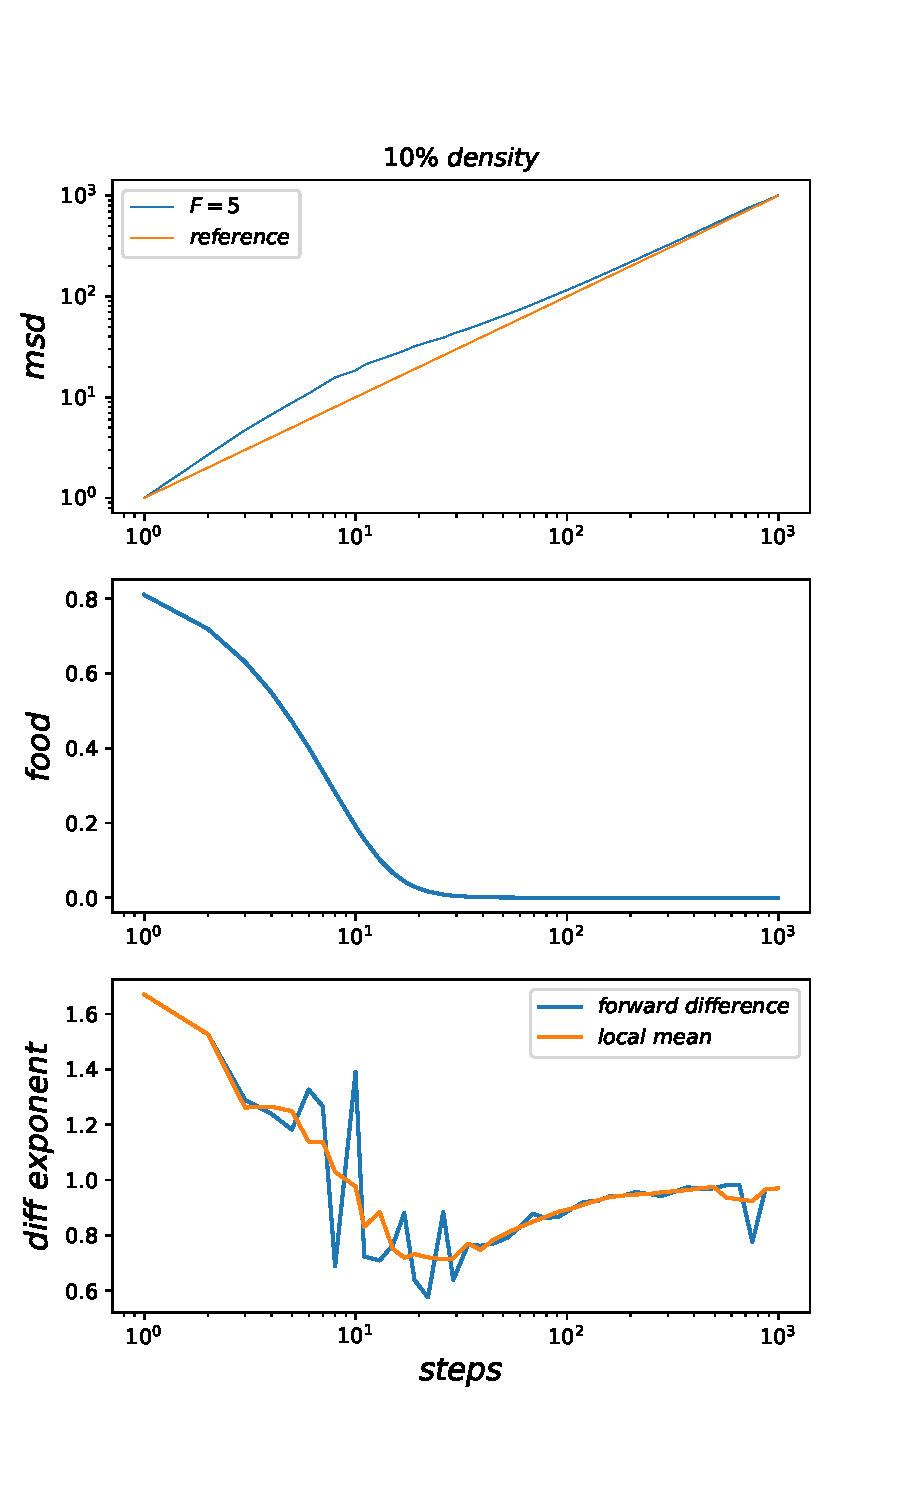
\includegraphics[scale=0.7]{10percent_free.pdf}
	\caption{$msd$, Nahrungsvorrat und (doppelter) Diffusionsexponent für 1000 Walker auf $100\times 100$ Nahrungsgitter gegen die Anzahl der (MC-) Schritte aufgetragen. Es wurden 100 Läufe und damit $10^5$ Samples verwendet.\label{food}}
\end{figure}




\subsection{Dichtekorrelation der Walker}
\noindent Um zu prüfen, wie sich der Abstand der Walker zueinander mit der Anzahl an Schritten verändert, wird eine vergröberte Dichtematrix eingeführt. Dazu wird die bisherige $100\times 100$-Matrix in $100$ $10\times 10$-Matrizen zerlegt und es wird die Besetzungszahl jeder dieser $10\times 10$-Matrizen in eine weitere $10\times 10$-Matrix geschrieben. Diese Matrix enthält nun die vergröberte Dichte der 100 ($10\times 10$)Blöcke aus denen die ursprüngliche Matrix besteht. 
\\
\noindent Das bedeutet, wir haben zu jedem Zeitschritt $i$ eine Matrix $\rho$ welche die Besetzungszahl der Blöcke enthält. Um eine über den 'Aufpunkt' gemittelte Abstands-Korrelation zu erhalten, bildet man (zu festem Zeitschritt $i$):
\begin{equation}
\hat{corr_i}(\Delta x,\Delta y) = \sum_{x_0,y_0}\rho_i(x_0,y_0)\cdot\rho_i(x_0+\Delta x,y_0+\Delta y)\ .
\end{equation}
Anschließend bietet es sich an, auf $\hat{corr_1}(0,0)$ zu normieren (damit Plots von 1 aus starten), also:
\begin{equation}
corr_i(\Delta x,\Delta y) = \frac{ \hat{corr_i}(\Delta x,\Delta y) }{ \hat{corr_1}(0,0) } \ .
\end{equation}
Die Implementierung sieht zu jeder fixen Zeit $i$ wie folgt aus, wobei $n$ hier eine Schleife über alle $N$ Walker ist.
\vspace{0.3cm}
\begin{figure}[H]
	\centering
	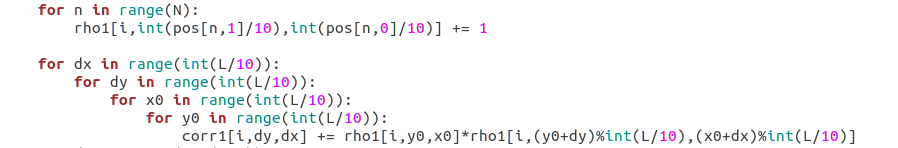
\includegraphics[scale=0.7]{corrcode.png}
	\caption{Implementierung der Korrelationsmatrix $\hat{corr_i}(\Delta x,\Delta y)$ zur Zeit $i$.}
\end{figure}

\newpage

\subsection{Dichteautokorrelation}\label{Dichteautokorr}
\noindent Im folgenden wird $corr_i(0,0)$ als Dichteautokorrelation eines Blocks bezeichnet, diese Größe gibt Auskunft über die Verteilung der Walker auf die Blöcke. Dies lässt sich leicht an einem kleinen Beispiel einsehen: man stelle sich eine $3\times 3$ Matrix vor, wo auf jedem Feld ein Walker sitzt, man erhält $\hat{corr}(0,0)=9$, befinden sich hingegen auf nur 3 Feldern je 3 Walker so ist $\hat{corr}(0,0)=27$. Das normieren skaliert nur die Achse, laufen Walker zusammen so steigt die Dichteautokorrelation, nähern sich die Walker einer Gleichverteilung, so sinkt die Dichteautokorrelation. Ich normiere auf die Startverteilung, man könnte auch auf die (best mögliche) Gleichverteilung normieren.
\\
\noindent Es wird die Selbstkorrelation für das System von 1000 Walkern auf dem $L=100$ Quadratgitter vorgestellt. Dazu wird wie oben erklärt das Gitter in 100 $10\times 10$ Blöcke unterteilt.
\\
\noindent Man erkennt deutlich, das die Dichteautokorrelation nach dem 2tem Schritt fällt, die Walker nähern sich also einer Gleichverteilung an, wo in jedem der 100 Blöcke genau 10 Walker wären.
\\
\noindent Dies bedeutet, dass trotz des gleichzeitigen Ziehens der Walker die Nahrung 'effizient geteilt' wird, nahe aneinander liegende Walker (welche also im selben Block sind) versuchen also in weniger stark belebte Blöcke zu wandern um mehr Nahrung zu bekommen.

\begin{figure}[h!]
	\centering
	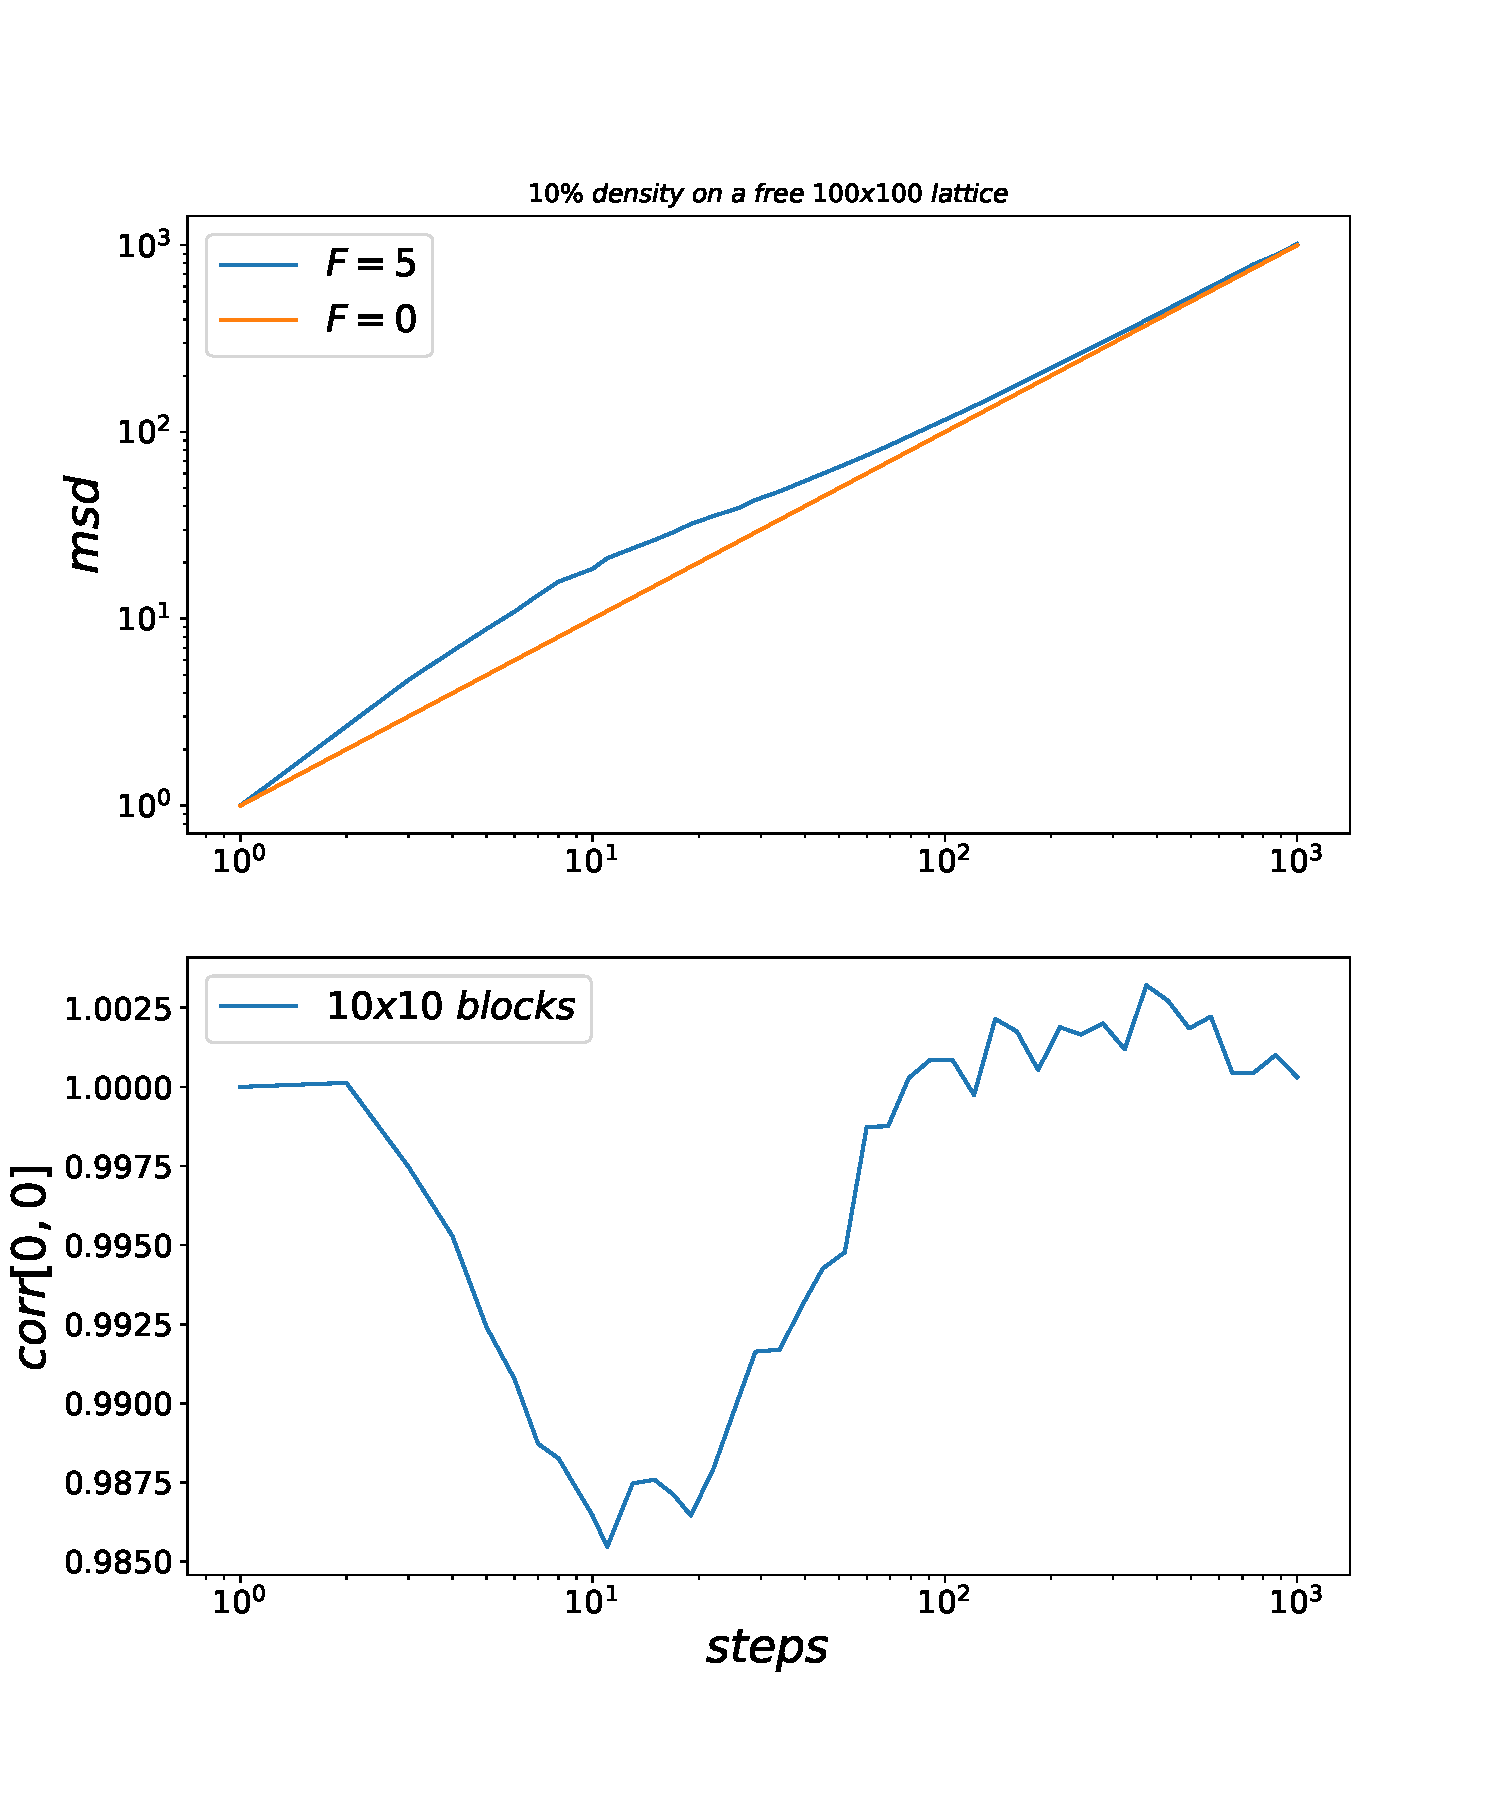
\includegraphics[scale=0.6]{autocorr10.pdf}
	\caption{Dichteautokorrelation für $10\times 10$ Blöcke bei einem System von 10\% Walkerdichte (auf $L=100$ Quadratgitter).}
\end{figure}

\clearpage

\subsection{Korrelation mit benachbarten Blöcken}

In diesem Abschnitt wird die Korrelation zu benachbarten Blöcken untersucht, dabei ist es unwesentlich, ob $\Delta x$ oder $\Delta y$ zu festen Zeitschritten $t$ variiert wird, aufgrund der Symmetrie des Systems (Invarianz unter Drehungen um $\pi/2$). Es wird in nachfolgenden Plots daher stellvertretend für beide Möglichkeiten $\Delta x$ variiert.

\begin{figure}[h!]
	\centering
	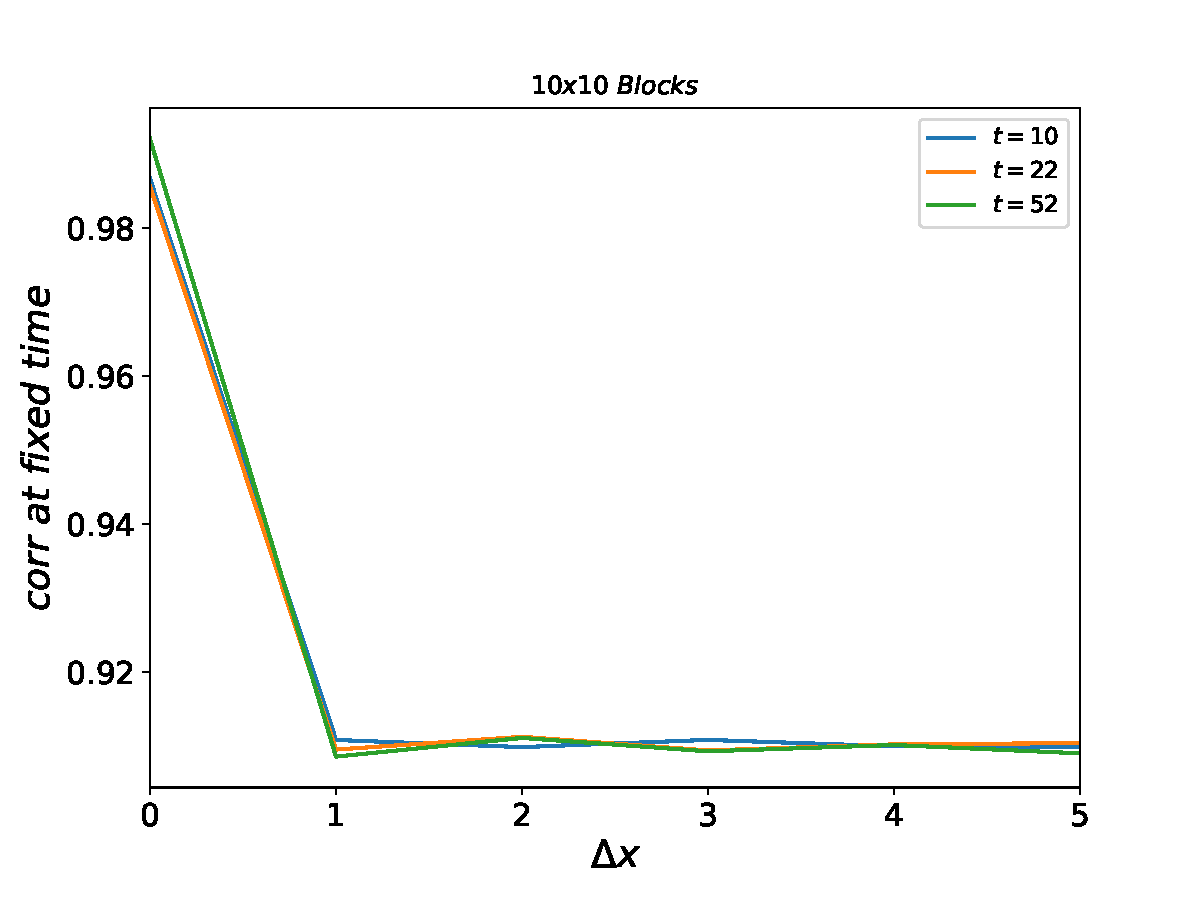
\includegraphics[scale=0.8]{dens10_corr10.pdf}
	\caption{Korrelation zu benachbarten Blöcken für eine Blockgröße von $10\times 10$.}
\end{figure}

\begin{figure}[h!]
	\centering
	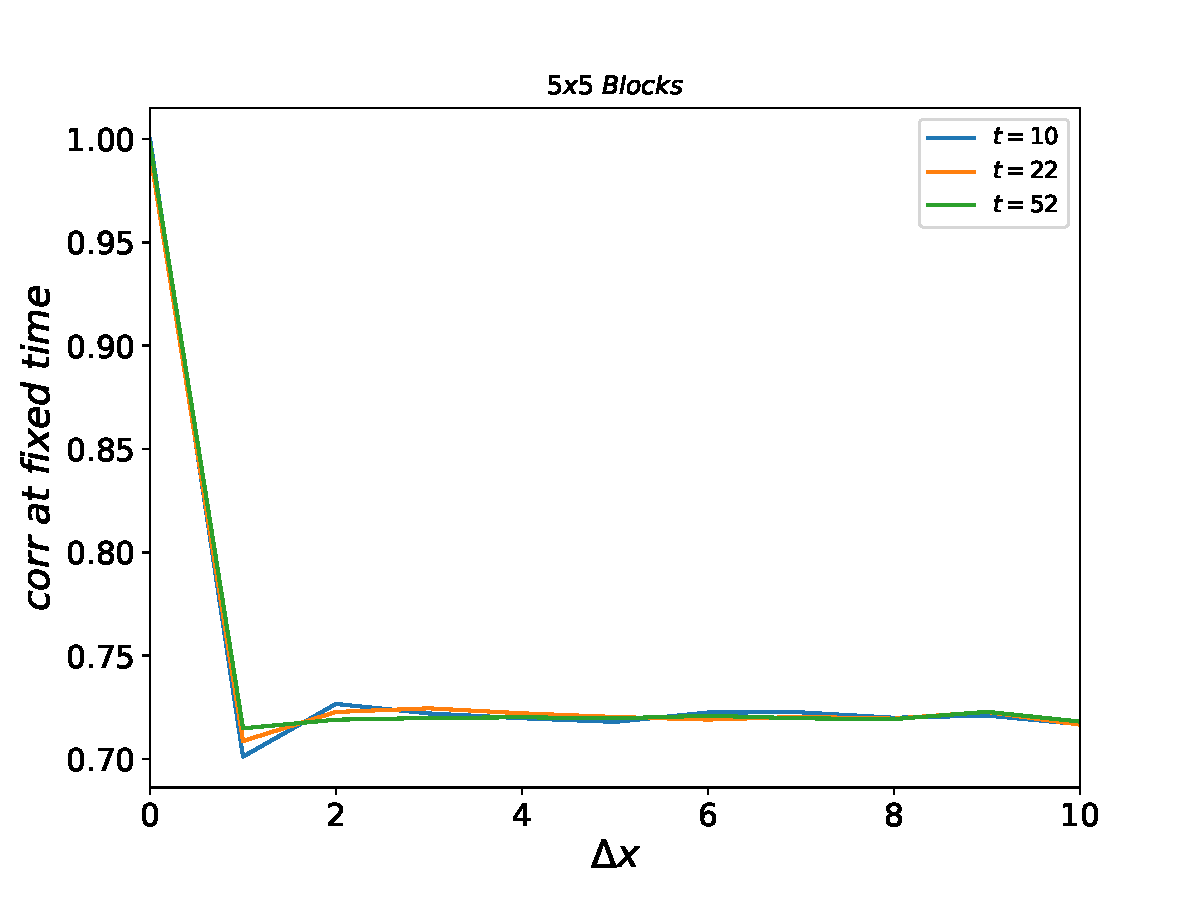
\includegraphics[scale=0.8]{dens10_corr5.pdf}
	\caption{Korrelation zu benachbarten Blöcken für eine Blockgröße von $5\times 5$.}
\end{figure}

\clearpage

\noindent Man kann an der oberen der beiden Abbildungen dieses Unterabschnitts sehen, das nach 10 Schritten, also etwa an der Stelle, wo der Super- auf Subdiffusion Übergang ist die Korrelation zum nächsten $10\times 10$ Block (von den drei hier verglichenen Zeitpunkten) am größten ist.
\\
\noindent Zudem sieht man, die Korrelation zum nächsten $5\times5$ Block ist (von den drei hier verglichenen Zeitpunkten) minimal ist. Der nächste $5\times 5$ Block wird also übersprungen. Dieses Ergebnis untermauert die Beobachtungen des vorangegangenen Unterschnitts, dass Walker aus stärker 'bevölkerten' stark 'abgestoßen' werden in weniger 'bevölkerte' Regionen des Nahrungsgitters.
\subsection{Autokorrelation der Schritte}
Gegenstand dieses Abschnitts ist es die Schrittautokorrelation des 2-dimensionalen nahrungssuchenden Random-Walks zu messen/simulieren. 
\\
Zur Erinnerung, die Schrittautokorrelationsfunktion ist definiert worden als:
\begin{align}
g_{t_0}(\tau) = \langle \hat{e}(t_0+\tau) \cdot \hat{e}(t_0) \rangle\ ,
\end{align}
wobei $\hat{e}(t)$ der Schritt zur Zeit $t$ ist. Der erste Schritt wird zur Zeit $t_0 = 0$ ausgeführt. Die nachfolgende Graphik zeigt genau genommen nicht $g_0(\tau)$ sondern $g_0$ in Abhängigkeit von der Anzahl der Schritte (wie schon im vorherigen Kapitel).
\\
Die Schrittautokorrelationsfunktion gibt an, wie stark jeder Schritt eines Walkers nach einer Anzahl von Schritten noch zu seinem ersten Schritt korreliert ist. Diese Korrelation wird natürlich durch die Nahrung induziert und verrät, ab wann diese keinen Effekt mehr hat und der Walk sich dem normalen Random-Walk annähert.
\\
\\
Eine weitere Graphik zeigt die Schrittautocorrelationsfunktion (erneut für 10\% Walkerdichte) bei verschiedenen Nahrungspropensitäten $F=0,1,2,5$. Man erkennt sehr deutlich, dass je größer $F$ ist, desto stärker und länger sind die Schritte korreliert.

\begin{figure}[H]
	\centering
	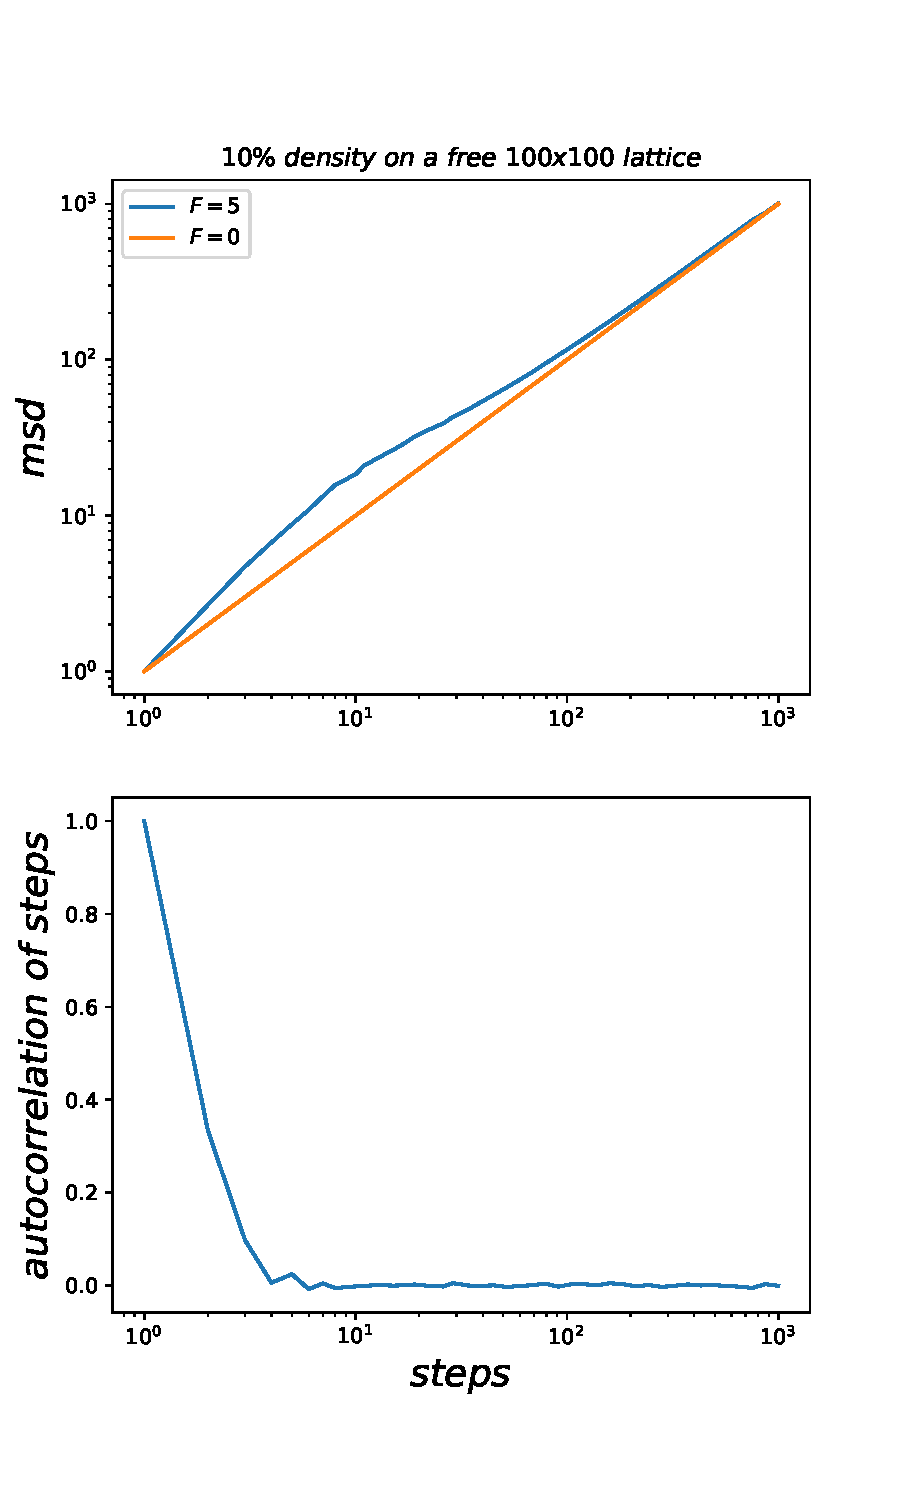
\includegraphics[scale=0.7]{dens10_escp.pdf}
	\caption{Autokorrelation der Schritte im Vergleich mit dem $msd$.}
\end{figure}

\clearpage

\begin{figure}[H]
	\centering
	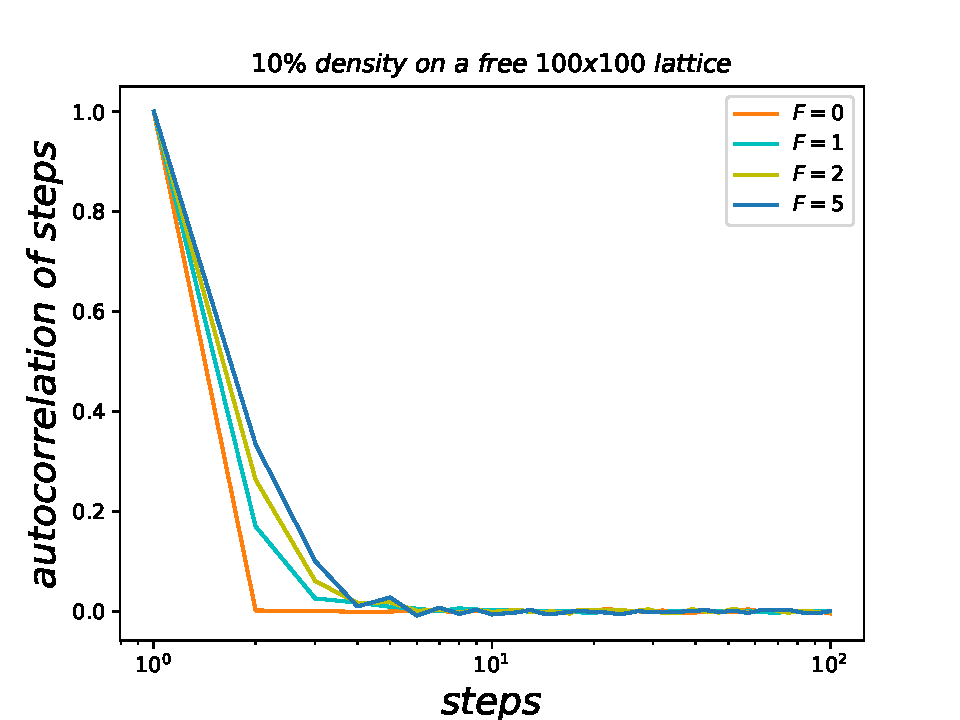
\includegraphics[scale=0.7]{stepautocorr_multF.pdf}
	\caption{Schrittautocorrelationsfunktion zu $F=0,1,2,5$}
\end{figure}

\clearpage

\section{Sukzessives Ziehen}
In diesem Abschnitt wird, im Gegensatz zu dem vorhergegangenen Abschnitt \ref{gleichzeitig}, der sukzessive Ziehalgorithmus der Walker (also ein Walker nach dem anderen, wobei nach jedem einzelnen Walker die Nahrungsmatrix bearbeitet wird) verwendet. Es werden die Ergebnisse mit denen, für gleichzeitiges Ziehen, verglichen.
\subsection{Mean-Squared-Displacement und Nahrungsvorrat}
Analog zu dem vorheigen Kapitel schaut man sich das $msd$ und den Nahrungsvorrat für den Prozess von 1000 'hungrigen' ($F=5$) Walkern auf einem mit Nahrung beöegten $100\times 100$ Gitter an. Es werden 100 Läufe simuliert um über $10^5$ Samples zu mitteln. Die Ergebnisse 

\begin{figure}[H]
	\centering
	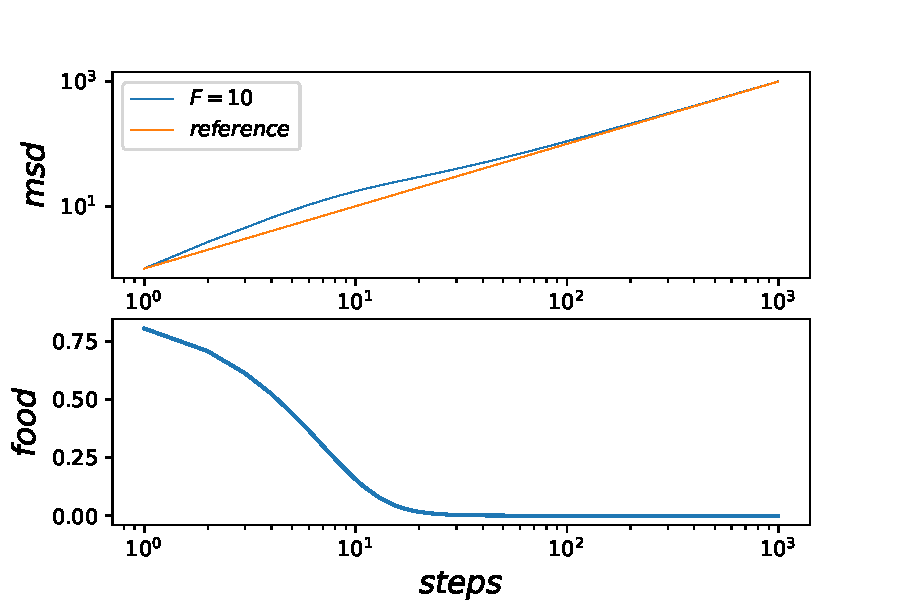
\includegraphics[scale=0.85]{suc10.pdf}
	\caption{$msd$ und Nahrungsvorrat für sukzessives Ziehen von 1000 Walkern auf $100\times 100$ Nahrungsgitter gemittelt über 100 Läufe (also $10^5$ Samples). 'reference' bezeichnet wie gehabt die freie Diffusion mit $D=1/4$, also $msd(t)=t$.}
\end{figure}

\clearpage

\noindent Man erkennt erst bei etwas näherer Betrachtung, dass die Nahrung etwas schneller abnimmt. Dementsprechend flacht auch das $msd$ früher ab und 'landet' früher auf der freien Diffusionskurve. 
\\
\noindent Die Erklärung für diesen Unterschied der beiden Algorithmen ist in einer Dimension klar, dort würden zwei Walker, die sich auf demselben Gitterplatz befinden (nahezu, zu ungefähr 99\%) immer in entgegengesetzte Richtungen ziehen, wenn um sie herum, also zu beiden Seiten, Nahrung vorhanden ist. Ziehen die Walker gleichzeitig so ziehen sie zu 50\% zusammen in eine Richtung und 'müssen die Nahrung teilen'.
\\
\\
\noindent Ein wirklicher/systematischer Unterschied ist aber zwischen den beiden Algorithmen bei mittleren und vorallem geringen Dichten (die hier untersucht werden) nicht zu erwarten, der sukzessive Algorithmus hat quasi einfach eine etwas höhere effektive Dichte.

\section{Mean-Squared-Displacement bei unterschiedlichen Walkerdichten}  
In diesem Abschnitt wird der Einfluss der Walkerdichte auf das $msd$ diskutiert. 
\\
Man kann vermuten, dass bei höherer Dichte schneller der 'Knick' hin zur Diffusionskurve entsteht. Denn der mittlere Abstand zwischen den hungrigen Walkern skaliert mit $N^{-1/2}$, wobei mit $N$ die Anzahl der Teilchen bezeichnet wird. Wenn also die Anzahl der Walker, und damit die Dichte, vervierfacht wird, so erwartet man das der mittlere Abstand sich halbiert.
\\
In anderen Worten, die mittlere freie Fläche ist linear zur Teilchenzahl $N$, das $msd$, also die vom Walker abgedeckte Fläche, wächst in der Kurzzeitdiffusion ungefähr wie bei dem SAW, also mit Exponenten $1.5$. Für die Lokalisierungsdauer, damit ist die Anzahl an Schritten bis die Walker sich (beziehungsweise die Fressspuren der anderen) 'sehen' gemeint, gilt somit:
\begin{align}
t_{loc} \sim \rho^{-2/3}\ ,
\end{align}
wobei $\rho$ die Walkerdichte bezeichnet.
\\
Bei doppelter Dichte sollte der 'Knick' hin zur Diffusionskurve also etwa nach dem $0.6$-fachen der Anzahl an Schritten eintreten, bei vierfacher Dichte nach $0.4$ facher Schrittanzahl.
\\
Diese Überlegungen gelten --wenn überhaupt-- natürlich nur für mittlere Dichte, nehmen wir eine Dichte von 200\% an, so ist mit hoher Wahrscheinlichkeit nach dem ersten Zug alle Nahrung 'verbraucht' und eine weitere Verdoppelung der Dichte bewirkt keinen Unterschied in der Zeit, dieses Phänomen ist auf die diskrete Natur des zugrundeliegenden Prozess zurückzuführen.



\section{Mean-Squared-Displacement mit neuem Aufpunkt}
Ausgehend von der vorangegangenen Beobachtung, das der Knick hin zur Diffusionskurve gleichzeitig mit dem Verschwinden der Schrittautokorrelationsfunktion eintritt, lässt sich vermuten, dass der subdiffusive Bereich nur eine Folge des superdiffusiven Beginns ist. Um diese Vermutung weiter zu Untermauern wird der Aufpunkt des $msd$ gewechselt.
\\
Es wird erneut ein Simulationsgitter mit Nahrung befüllt und der gleiche (biased) Random-Walk läuft ab, nur wird nun erst nach $t_0$ Schritten das $msd$ aufgenommen. Es ist also der hier als erste Schritt dargestellte Schritt 'in Wirklichkeit' der $t_0+1$te Schritt, aber der Aufpunkt wird um $t_0$ Schritte verschoben, in Formeln also:
\begin{align}
msd_{t_0}(t) = \langle \left[\vec{r}(t-t_0)-\vec{r}(t_0)\right]^2\rangle\ ,
\end{align}
wobei hier dann natürlich $\langle ... \rangle$ das Ensemblemittel ist.
\\
Es lässt sich nun sehen, ob jetzt schon einfach ein normaler Random-Walk stattfindet, oder ob tatsächlich kurzzeitig eine anomale Diffusion mit tatsächlich langsamerer Ausbreitung der Walker vorliegt.
\\
Die nachfolgende Graphik zeigt das Simulationsergebnis von 1000 (Dichte ist also 10\%) hungrigen Walkern auf dem mit Nahrung belegten freien $L=100$ Gitter mit einem Zeitshift von $t_0=10$ mit dem gleichzeitig ziehenden Algorithmus untersucht. Ich wähle $t_0=10$ deshalb, da an dieser Stelle zuvor (siehe 4.2.6) ein starker Knick hin zur Diffusionskurve war und somit der doppelte Diffusionexponent deutlich unter 1.

\begin{figure}[H]
	\centering
	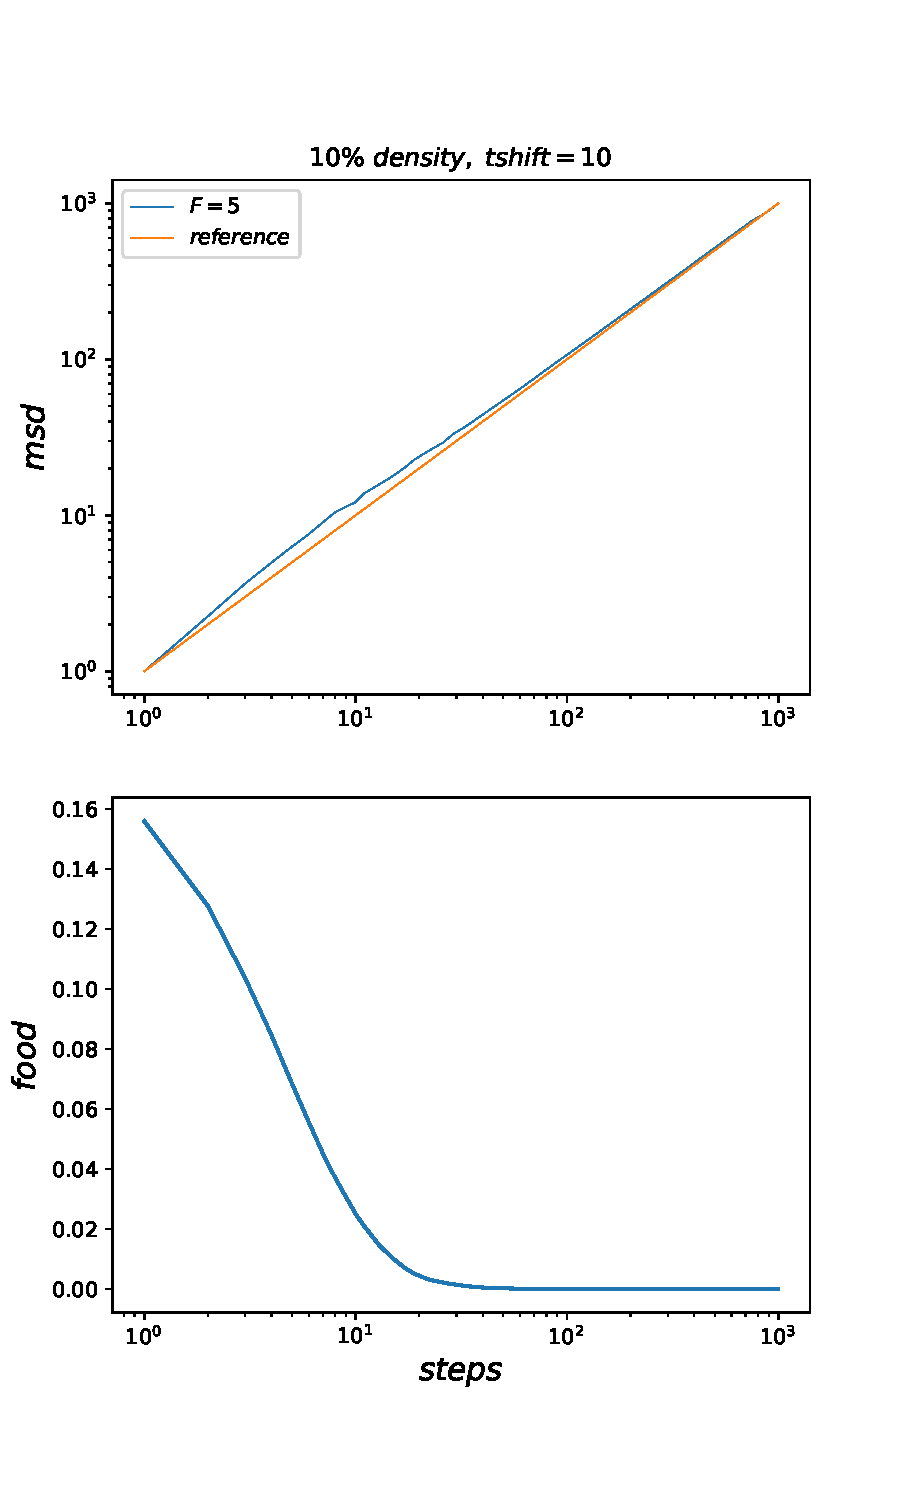
\includegraphics[scale=0.75]{tshift10.pdf}
	\caption{$msd_{t_0=10}$ bei 10\% Walkerdichte auf dem freien $100\times100$ Gitter belegt mit Nahrung, im Vergleich zu dem freien 2D Random-Walk $msd(t)=t$.}
\end{figure}
\clearpage

\noindent Man erkennt nun eindeutig, das der zuvor subdiffusive Bereich plötzlich superdiffusiv ausschaut, legen wir an den zuvor elften und zwölften Schritt ein Steigungsdreick an, so ist die Steigung deutlich kleiner als 1, legen wir hier an den ersten und zweiten Schritt ein Steigungsdreieck an, so ist die Steigung deutlich über 1.
\\
Die Walker breiten sich also nicht langsamer als die Diffusion in diesem Bereich aus, sondern eigentlich sogar etwas schneller. Da die Walker aber zuvor viel schneller waren (also sich viel stärker ausgebreitet haben) und somit schon deutlich größere mittlere Abstände zum jeweiligen Startpunkt haben, sieht es im $msd$ Plot aus, als würden sich die Walker weniger als diffusiv ausbreiten.
\\
Dies zeigt also, dass lokale Exponenten in transienten $msd$'s mit Vorsicht zu interpretieren sind. In Kapitel 6 wird die Diskussion vertieft und mit weiteren ähnlichen Beispielen (etwa \cite{Zausch_2008}) in Zusammenhang gestellt.

\chapter{Viele Random-Walker auf dem perkolierenden Cluster mit Nahrung (2D)}
In diesem Kapitel wird die Dynamik vieler 'hungriger' Random Walker auf dem perkolierenden Cluster untersucht. Es wird also das 'Clearing out a Maze' Paper auf viele Walker erweitert. Wie zuvor besteht zwischen den Walkern keine direkte Interaktion, sondern nur indirekt über 'Wegfressen' der Nahrung.
\\
\noindent Auf dem freien Cluster wurde gefunden, dass die Dynamik nach einem superdiffusiven Regime zu Beginn in ein subdiffusives Regime wechselt (d.h. der Diffusionsexponent $2\nu$ ist kleiner 1 und das $msd$ liegt unter dem der freien Diffusion). Das $msd$ nähert sich also auf lange Zeiten dem der freien Diffusion ($F=0$) von oben an.
\\
\noindent Auf dem perkolierenden Cluster gibt es zwei Vergleichskurven, der einzelne Walker mit Nahrung auf dem perkolierenden Cluster ('Clearing out a Maze') und der Fall $F=0$ also die anomale Diffusion auf dem perkolierenden Cluster ($\nu \approx 0.347$ in zwei Raumdimensionen).
\\
\noindent Zu beachten ist, dass der perkolierende Cluster immer unterschiedlich groß ist und daher unterschiedlich viele Walker für die gleiche Dichte benötigt werden. Hier wird bei der so errechneten Anzahl der Walker immer abgerundet (mittels der int()-Funktion in Python3).

\section{Simulation von 10\% Walkerdichte auf dem perkolierenden Cluster}
In diesem Abschnitt werden $msd$, Nahrungsvorrat und besonders der (doppelte) Diffusionsexponent von vielen Walkern auf dem perkolierenden Cluster diskutiert. Die Anzahl Gitterplätze auf dem perkolierenden Cluster in einem $100\times 100$ Gitter beträgt etwa 4000 (kann aber auch 2500 oder 5500 sein), somit befinden sich etwa 400 hungrige Random-Walker (PAC-MANs) auf dem perkolierenden Cluster. 
\\
\noindent Man erwartet zu beginn die aus \cite{doi:10.1063/1.4999485} bekannte Kurzzeitdiffusion, da die PAC-MAN's sich die ersten paar Schritte bei dieser Dichte wohl nicht 'sehen', sie bemerken nicht die Fressspuren der anderen, da ihr mittlerer Abstand am Anfang zu groß dafür ist. Auf lange Zeiten erwartet man die anomale Diffusion auf dem perkolierenden Cluster aus \cite{PhysRevLett.50.77}, da irgendwann einmal alle Nahrung 'aufgefressen' worden ist und nun keine Interaktion mehr zwischen den Walkern ist und auch die einzelnen Walker nicht mehr durch die Nahrung beeinflusst werden.
\\
\noindent In diesem Abschnitt wird geprüft, ob dieses vermutete Verhalten eintritt und vor allem, wann der 'Wechsel der Kurven' stattfindet, also ob die Langzeitdiffusion der Ein-PAC-MAN Dynamik aus \cite{doi:10.1063/1.4999485} erreicht wird oder nicht. Aus diesen Simulationsergebnissen kann man dann weitere Vorhersagen treffen, bei welcher Dichte wohl ein Wechsel der Langzeitdiffusionskurven zu erwarten ist.


\begin{figure}[H]
	\centering
	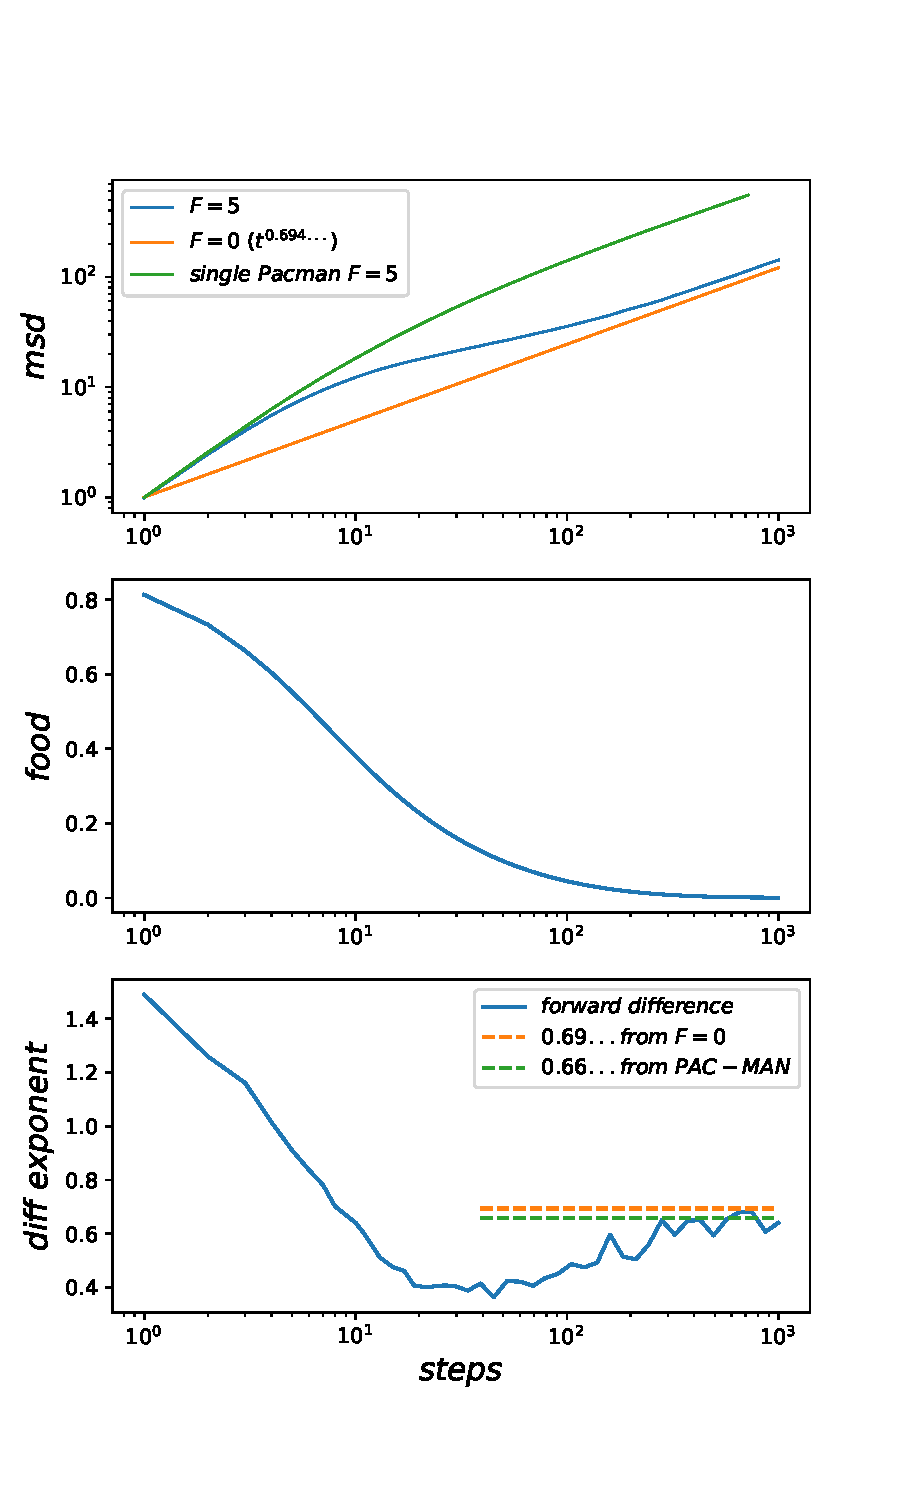
\includegraphics[scale=0.75]{10percent_on_pc_new_version.pdf}
	\caption{Oben beschriebenes Modell von 10\% Walkerdichte auf perkolierendem Cluster.
	Es wurden 1
	50 Matrizen/Cluster mit je 50 Läufen simuliert um (bei im Schnitt ca. 400 Walkern) über $10^5$ Samples zu mitteln.  }
\end{figure}

\clearpage

\noindent Die Simulationsergebnisse zeigen, dass die Langzeitdiffusion mit 'neuem' Exponenten (aus \cite{doi:10.1063/1.4999485}) nicht erreicht wird. Es wird vorher, aufgrund mangelnder neuer Nahrung welche die Walker 'biased', auf die 'klassische' anomale Diffusionskurve des perkolierenden Clusters (also ohne Nahrung) gewechselt. Nach 8-10 Schritten ist der Wechsel deutlich zu sehen und es liegen dort noch etwa 60\%-40\% der Nahrung vor. 
\\
Diese Simulation dient gut zur Abschätzung, dass deutlich geringe Dichten gewählt werden müssen um tatsächlich in die PAC-MAN Langzeitdiffusion zu gelangen und anschließend aufgrund fehlender Nahrung auf die $F=0$ Kurve zu wechseln. 
\\
Statt nach 8-10 Schritten, soll erst nach ca 100 Schritten der Nahrungsvorrat soweit geschrumpft sein, das die PAC-MAN Kurve 'verlassen wird'. Es braucht also eine Walkerdichte von etwa 1\% oder auch 0.5\%, dies wären also im Fall des $100\times100$ Simulationsgitter etwa 40 (beziehungsweise 20) Walker.


\section{Mean-Squared-Displacement bei unterschiedlichen Walkerdichten} 
Wie zuvor angekündigt wird in diesem Kapitel zunächst das Simulationsergebnis für das gleiche System wie im vorigen Kapitel, aber bei einer sehr geringen Walkerdichte von 0.5\%, vorgestellt.
\\
Anschließend wird wie auf dem freien Gitter (ohne geblockte Plätze) eine Graphik mit verschiedenen Dichten und Referenzsystemen vorgestellt.
\\
\\
Die Hoffnung bei einer Walkerdichte von 0.5\% war, dass das $msd$ in den Bereich der sogenannten PAC-MAN Langzeitdiffusion kommt, also eine ano
male Diffusion mit einem von der Nahrungspropensität $F$ abhängigen Diffusionsexponenten ('power-law') unterhalb dem für denn klassischen Random-Walk auf perkolierendem Cluster. Erneut wurde über etwa $10^5$ Samples gemittelt.

\begin{figure}[H]
	\centering
	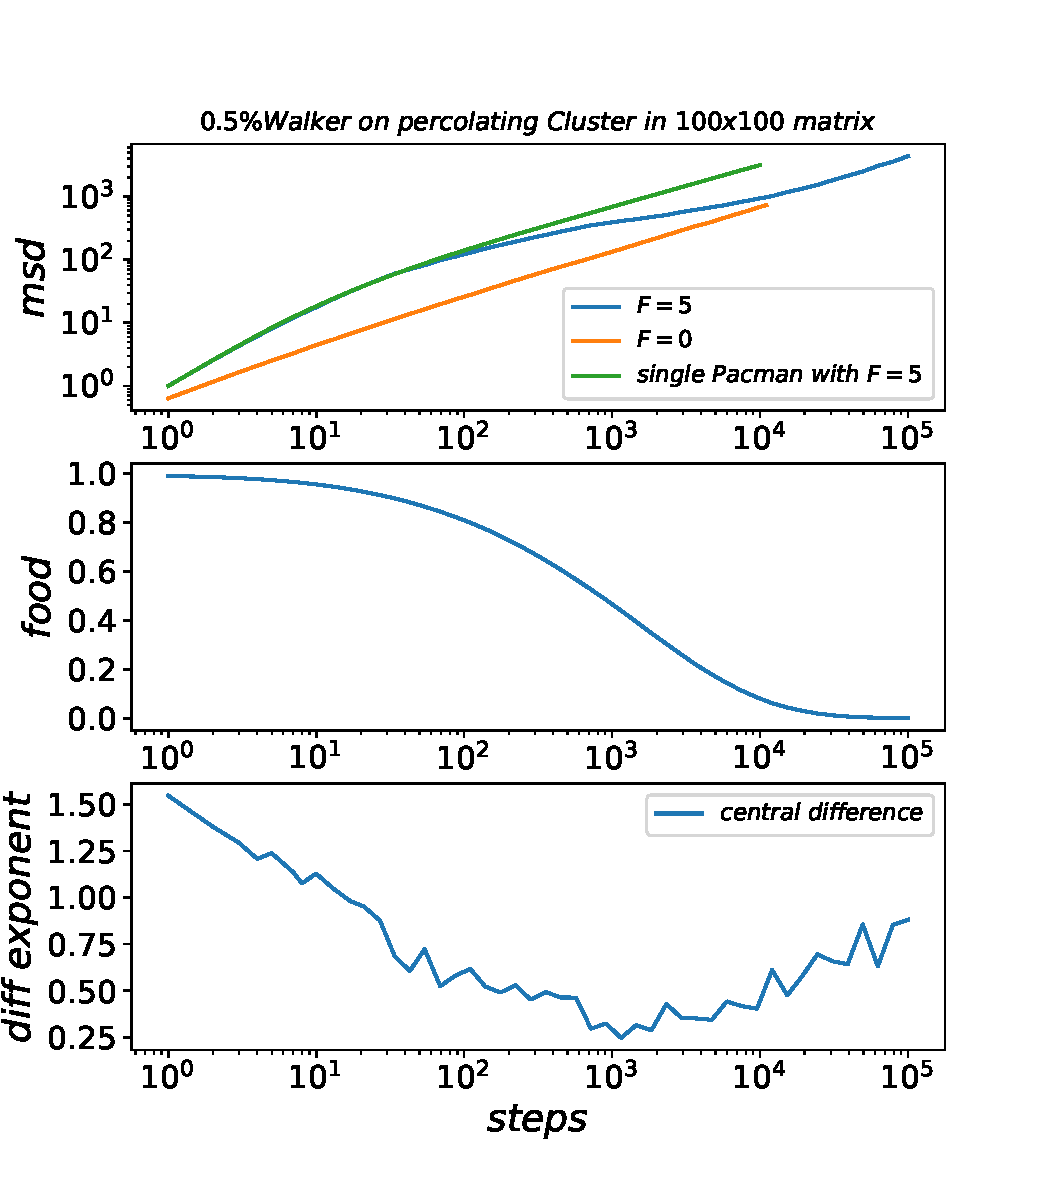
\includegraphics[scale=0.75]{05percent_on_pc.pdf}
	\caption{Oben beschriebenes Modell von 0.5\% Walkerdichte auf perkolierendem Cluster.
		Es wurden 1
		50 Matrizen/Cluster mit je 100 Läufen simuliert um (bei im Schnitt ca. 20 Walkern) über $10^5$ Samples zu mitteln.  }
\end{figure}

\clearpage

\noindent Nun wird tatsächlich die PAC-MAN Langzeitdiffusion erreicht. Zu Beginn dieser Arbeit wurde diese diskutiert und insbesondere wieso die Ausbreitung durch das Einführen der Nahrung, also ein starkes bevorzugen zuvor nicht-besuchter Plätze, langsamer wird. Das schlagende Argument war, dass der hungrige Walker (PAC-MAN) im gegensatz zu einem normaler Random-Walker auf dem perkolierenden Cluster häufiger in Sackgassen (oder auch 'tote Enden' genannt) gezogen wird als der normale Random-Walker und sich anschließend langsam/diffusiv aus diesen 'herauskämpfen' um wieder auf dem sogenannten 'Backbone' des perkolierenden Clusters zu sein. 
\\
Ich gebe in dieser Arbeit ganz bewusst keine genauere Definition des 'Backbone' außer, das dieser der Bereich des perkoliernden Clusters ist, der zum schnellen Durchschreiten geeignet ist. Viele in der Literatur zu findende Definition und gar Algorithmen um dieses 'Backbone' zu finden sind mit großer Vorsicht zu genießen und enthalten einige Unstimmigkeiten. Der 'Backbone' wird oft als der Bereich in dem der Strom bei beliebigem Blitzeinschlag auf dem perkolierenden Cluster abfließen würde definiert und so auch bestimmt. Problematisch ist der beliebe Einschlagpunkt, liegt dieser in einem toten Ende oder in einem Umweg (eine loop oder ähnliches) so zählt man dies mit zum 'Backbone'. 
\\
\\
Es gibt hier also einen fundamentalen Unterschied zum freien Cluster, das die Langzeitdiffusion durch das Einführen von Nahrung 'langsamer' wird. Hier könnten also tatsächlich überproportional viele Walker in Sackgassen laufen und die Ausbreitung verlangsamen. 
\\
Diese Frage wird im nächsten Kapitel wieder durch eine veränderte Aufpunktwahl, wie schon in der freien Ebene, versucht zu klären.
\\
\\
Um diesen Abschnitt abzuschließen wird eine Graphik mit verschiedenen Walkerdichten auf dem perkolierenden Cluster gezeigt, die Dichte beeinflusst erneut den Zeitpunkt zu dem auf die Langzeitreferenzkurve ohne Nahrung gewechselt wird. Denn die Anzahl der Walker bestimmt natürlich wie lange wie viel Nahrung vorhanden ist.

\begin{figure}[H]
	\centering
	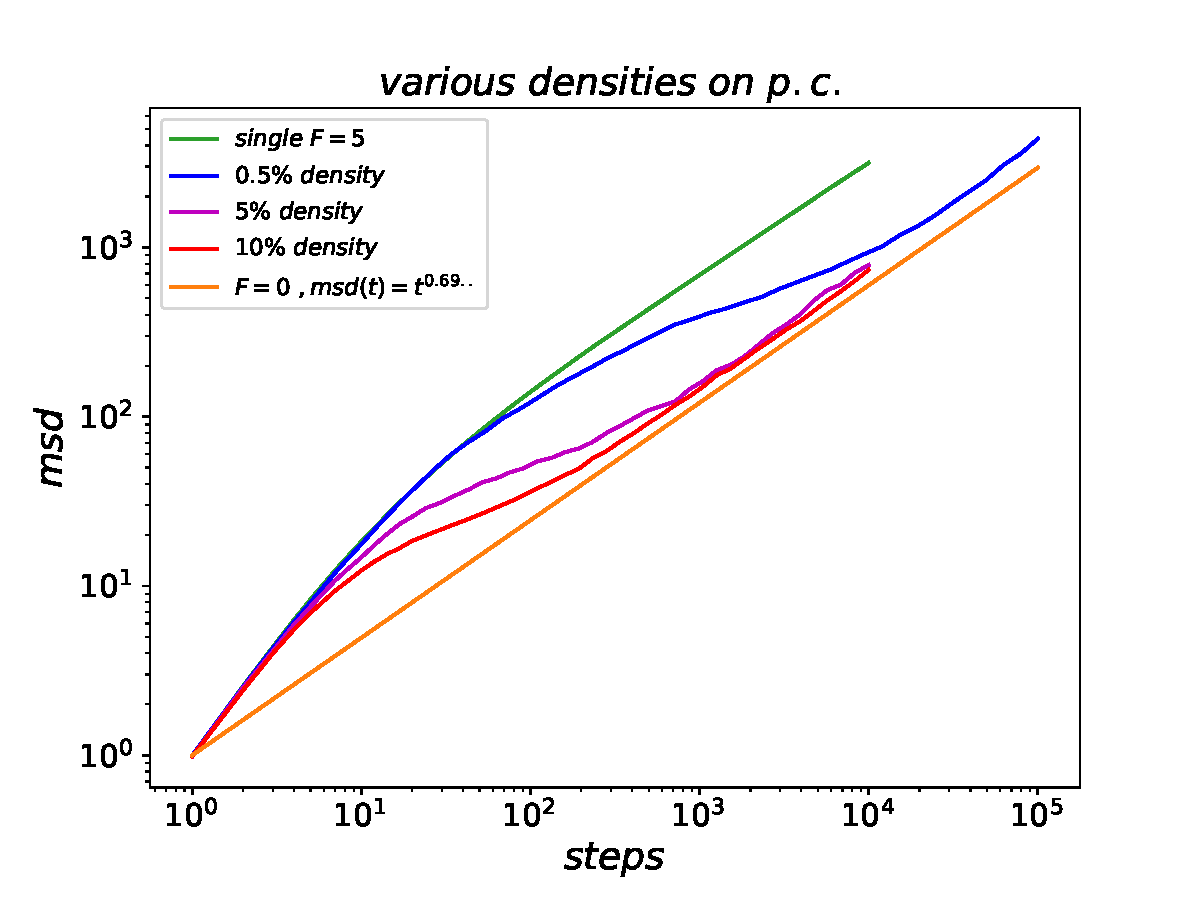
\includegraphics[scale=0.75
	]{vardenspc.pdf}
	\caption{$msd$ zu verschiedenen Walkerdichten auf dem perkolierenden Cluster im Vergleich zur Ein-Teilchen PAC-MAN Dynamik und zum $F=0$ Fall, also dem klassischen Random-Walk auf dem perkolierenden Cluster ohne Nahrung.}
\end{figure}

\section{Mean-Squared-Displacement auf dem perkolierenden Cluster mit neuem Aufpunkt}
Die Simulation des 'biased' Random-Walk durch Nahrung ('PAC-MAN' Walk) auf dem perkolierenden Cluster, mit mehreren indirekt interagierenden Walkern hat gezeigt, dass je nach Dichte der Walker verschieden lange das in \cite{doi:10.1063/1.4999485} gefundene $msd$ gehalten wird. Es wird je nach Dichte subdiffusiv (also mit geringerem Diffusionsexponenten als der freie Random-Walk in gleicher Umgebung) auf die freie $F=0$ Kurve gewechselt. Ähnlich wie auf dem freien Nahrungsgitter soll nun auch hier dieser Bereich durch neue Aufpunktwahl des $msd$ untersucht werden. Durch diesen Wechsel des Aufpunktes lässt sich die Ausbreitung aus dem zu diesem Zeitpunkt vorliegenden Zustand (also Walker und Nahrungsverteilung) messen.
\\
Wir nehmen hier erneut die 0.5\% Dichte (auf dem $L=100$ Simulationsgitter) und verschieben den Aufpunkt einmal um 100 Schritte, denn dort beginnt der Walker etwa die 'PAC-MAN-Kurve' zu verlassen und unter den $F=0$ Exponenten von $2\nu \approx 0.694...$ zu fallen.
\\
Zudem wird an gleichem System eine Simulation mit um 1000 MC-Schritte verschobenem Aufpunkt durchgeführt, also in dem Bereich zwischen den beiden Referenzkurven (PAC-MAN und $F=0$).
\\
Abschließend wird noch einmal das System mit einem um 10000 Schritte verschobenem Aufpunkt betrachtet, also zu einem Zeitpunkt wo das ursprüngliche $msd$ auf der $F=0$ Referenzkurve liegt.
\\
Durch diese drei Verschiebungen des Aufpunkte können Aussagen über die tatsächlichen Ausbreitungsgeschwindigkeiten der hungrigen Random-Walker getroffen werden.

\begin{figure}[H]
	\centering
	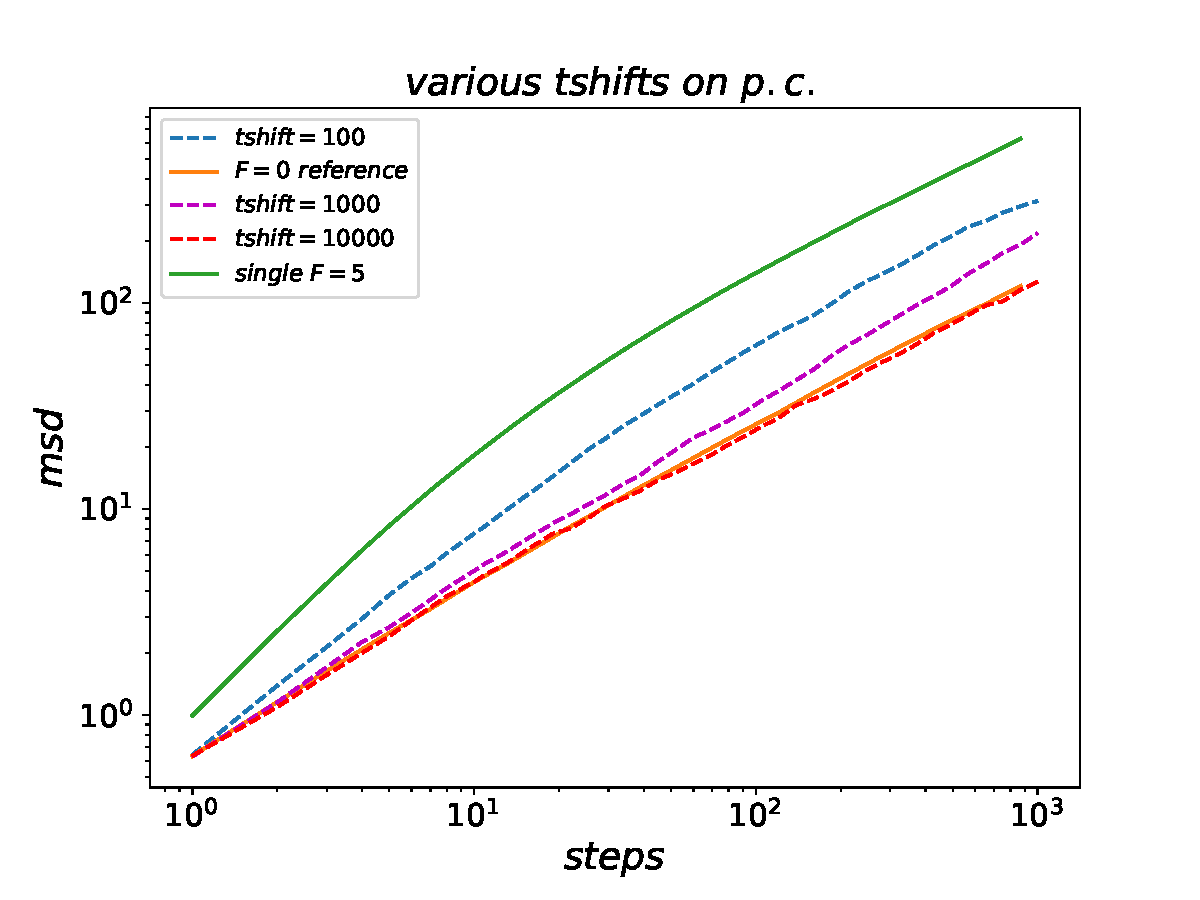
\includegraphics[scale=0.6]{tshift_pc.pdf}
	\caption{$msd$ zu verschiedenen verschobenen Aufpunkten im Vergleich zu der PAC-MAN Kurve und der $F=0$ Referenz (anomale Diffusion auf dem perkolierenden Cluster).}
\end{figure}

\clearpage

\noindent Es ist, sehr Ähnlich wie in Kapitel 4 auf dem freien Gitter ohne Hindernisse, zu sehen, dass keine echte Subdiffusion stattfindet, erneut scheinen die Walker sich nur der $F=0$ Referenz anzupassen. Ihre Ausbreitung ist auch nach 100 und 1000 Schritten (wo noch jeweils ungefähr 80\% und 40\% der Nahrung vorhanden sind) noch immer schneller als die Referenz völlig ohne Nahrung. Diese ergibt sich auch nach 10000 Schritten, bei unter 20\% Nahrungsvorrat wieder.
\\
Letzteres Ergebnis stellt die Aussage von \cite{doi:10.1063/1.4999485}, dass durch die Nahrung die Walker mehr Zeit als 'üblich' (also ohne Nahrung) in Sackgassen/toten Enden des perkolierenden Clusters verbringen in Frage. Denn wären tatsächlich mehr Walker als 'üblich' in Sackgassen, so kann man erwarten, dass diese Verteilung auch nach einer großen Anzahl an Schritten vorliegt wo nahezu alle Nahrung weggefressen ist. Diese Startverteilung mit mehr Walkern in Sackggassen als üblich sollte zu einem $msd$ zwischen 'percolating-cluster average' und 'all-cluster average' führen. Diese Vermutung ist aber eine sehr vage und wird wie zuvor bereits erklärt nicht weiter diskutiert. Um Aussagen dieser Art zu diskutieren muss zuvor eine neue und strengere Definition des sogenannten 'Backbone' (siehe oben) gegeben werden und ein Algorithmus zum Auffinden dieses neu definierten 'Backbone' entwickelt werden, beide Aufgaben sollen kein Teil dieser Arbeit sein.

\chapter{Transiente Mean-Squared-Displacements}
\section{Beispiele für transiente msd}
Dieses Kapitel widmet sich transienten, also vergänglichen, mean-squared-displacements. Hiermit sind nicht stationäre, sich ständig verändernde, Prozesse wie in den beiden letzten Kapiteln untersucht gemeint. In diesen Prozessen kann es im $msd$ zu sub- oder superdiffusiven Bereichen kommen, ohne jedoch das dies die tatsächliche Ausbreitungsgeschwindigkeit der Teilchen/Walker (oder eines einzelnen Teilchens/Walkers) korrekt beschreibt.
\\
So wurde zum Beispiel in Kapitel 4 ein subdiffusives Regime gesehen, in welchem man durch veränderte Aufpunktwahl des $msd$'s (numerisch durch Monte-Carlo-Simulation) zeigen konnte, dass sich die Walker weiterhin stärker als diffusiv aus ihrer aktuellen Konfiguration ausbreiten und unter diesem Aufpunkt sogar superdiffusive Dynamik aufweisen.
\\
Dieses Beispiel zeigt also schon, dass in Prozessen, welche nicht stationär sind sondern sich ständig mit der Zeit verändern, das $msd$ und auch insbesondere der unter Vermutung eines Potenzgesetzes/'power-law' bestimmte Diffusionsexponent $\nu$, beziehungsweise $2\nu$, nicht die volle Aussagekraft hat, die ihm oft (insbesondere in einführenden Vorlesungen über statistische Physik und Systeme weicher Materie) zugesprochen wird.
\\
\\
Ein weiteres sehr spannendes Beispiel für einen transienten Prozess ist die Dynamik von kolloidalen Flüssigkeiten unter Scherung, wie Beispielsweise in dem Paper \cite{Zausch_2008} diskutiert. Hier wird die Dynamik durch die Scherung vergänglich (transient) beeinflusst. Ein Kolloidales System nahe dem Glasübergang erfährt eine fortlaufende Scherung, ab einer bestimmten Stärke der Scherung wird eine superdiffusive Dynamik beobachtet, auch hier besteht die Frage, ob dieser Superdiffusion eine tatsächlich schnellere Ausbreitung der Teilchen zugrunde liegt. Oder dies nur ein Effekt der zuvor, bei geringer Scherung, zu langsamen Ausbreitung und anschließender Anpassung an die Diffusionskurve, welche auf lange Zeiten sich einstellen muss, ist.


\section{Minimalmodel eines Walkers auf einem Nahrungsquadrat, echte Subdiffusion}\label{minimalmodell}
Es wird nun im Gegensatz zu den vorherigen Modellen ein transienter Prozess vorgestellt, der zunächst superdiffusive Dynamik aufweist und anschließend ein echt subdiffusives Regime zeigt. Mit echt subdiffusivist eine $msd$ gemeint, welches tatsächlich unter der Diffusionenskurve liegt, zumindest nach Wahl des Aufpunktes zu Beginn dieses Regimes. Denn so kann man mit Gewissheit sagen, dass die Ausbreitung zu einem gewissen Zeitpunkt tatsächlich geringer ist als bei dem vergleichbaren Diffusionsprozess.
\\
Ein leicht zu verstehendes und auch leicht zu implementierendes Minimal\-modell, für einen solchen transienten Prozess, ist es einen einzelnen Walker in die Mitte eines kleinen mit Nahrung besetzten Quadrates innerhalb einer größeren Matrix zu setzen. Hier wird zum Beispiel in die Mitte einer $L=100$ Matrix ein $l=20$ Quadrat mit Nahrung belegt (das heißt auf die x und y Indices 40 bis einschließlich 59), der Walker startet bei $x_0=y_0=50$.

\begin{figure}[H]
	\centering
	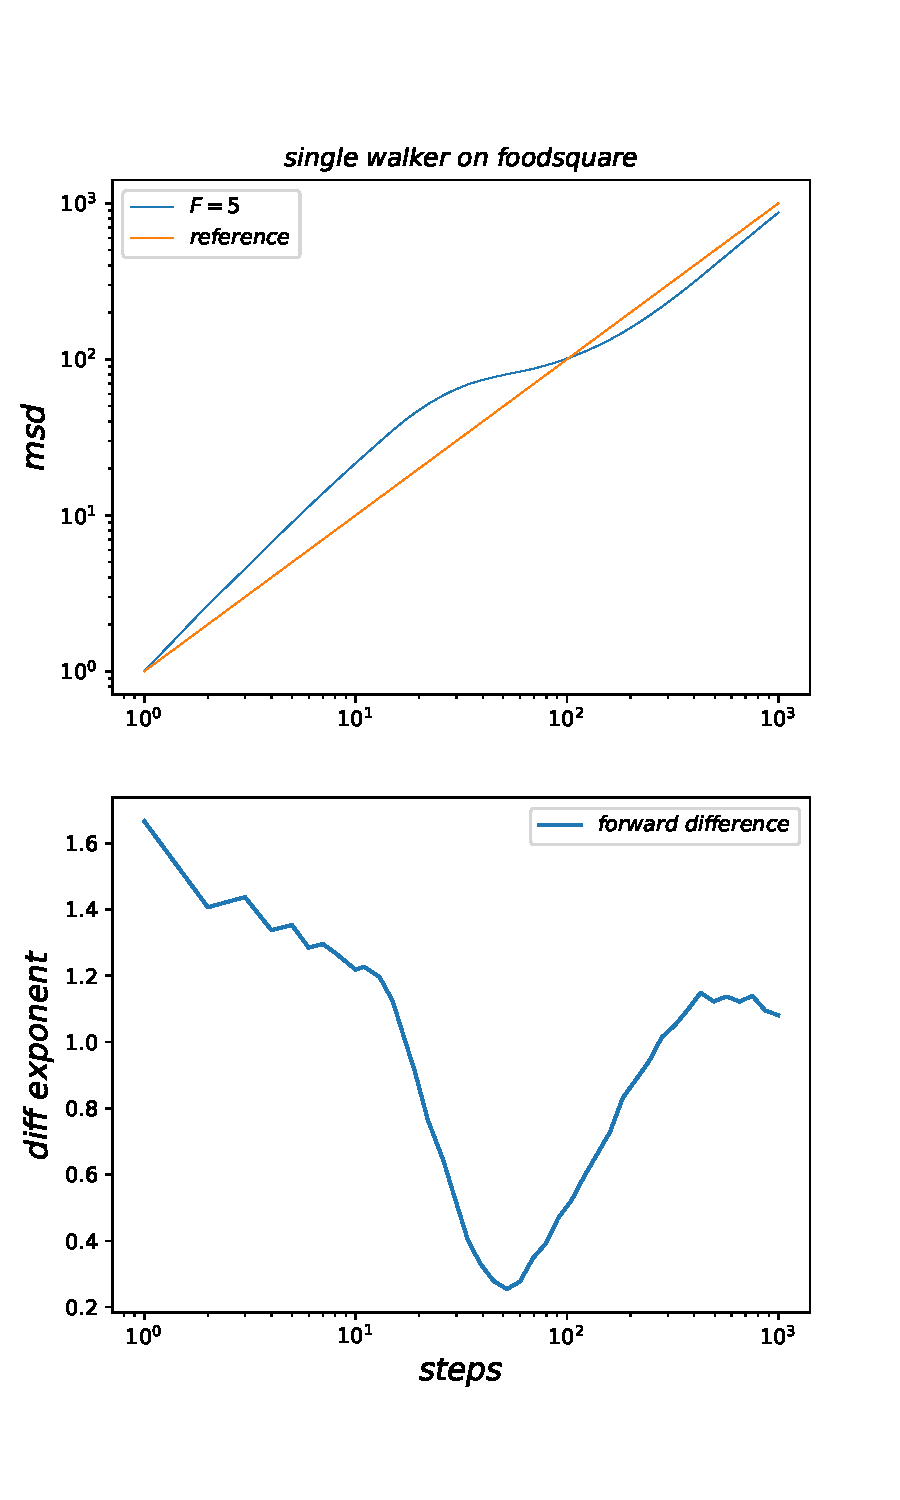
\includegraphics[scale=0.75]{single_walker_on20x20.pdf}
	\caption{Ergebniss der MC-Simulation des oben vorgestellten Minimalmodells. Es wurde über $10^5$ Samples gemittelt.}
\end{figure}


\noindent Es ist in der nachfolgenden Abbildung zu sehen, dass der Walker bei etwa $\sqrt{msd} \approx 10$ streng subdiffusiv wird, dies passt genau mit dem Erreichen von dem Rand des Nahrungsquadrat zusammen. Nach ungefähr 200 bis 300 MC-Schritten läuft der Walker wieder fast diffusiv, beziehungsweise sogar leicht superdiffusiv (siehe unten), da er sich 'freigefressen' hat, das Nahrungsquadrat ist nahezu leer und der Walker hat kein mit Nahrung benachbartes Feld um sich. 
\\
\\
Interessant ist es auch, zu erwähnen, dass nach dem subdiffusiven Regime wieder ein leicht superdiffusives Regime auftreten zu scheint. Nach den vorherigen Diskussionen ist es aber möglich, dass dem nicht der Fall ist, sondern dies erneut nur der umgekehrte Effekt von Kapitel 4 ist. Nach dem subdiffusiven Regime ist die Ausbreitung hinter der der normalen Diffusion zurück, ein anschließender normaler Random-Walk (da auch keine Nahrung mehr vorhanden ist, muss es sich um einen solchen handeln) erscheint hier superdiffusiv. Eine Verschiebung des Aufpunktes für das $msd$ um 300 Schritte zeigt, also in den Bereich, wo der doppelte Diffusionsexponent über $1.0$ zu sein scheint. Damit lässt es sich klären, ob tatsächlich eine Superdiffusion vorliegt und die Random-Walker sich stärker als diffusiv ausbreiten oder nur eine diffuives Verhalten, welches nur durch den 'Rückstand' gegenüber $msd(t)=t$ superdiffusiv erscheint.
\\
\\
\noindent
Die nachfolgenden Ergebnisse zur Simulation des $msd$'s mit um 300 Schritte verschobenem Aufpunkt bestätigen eine leichte Superdiffusion für ungefähr weitere 100 Schritte. Anschießend findet die übliche (wie schon in Kapitel 4 gesehen) Anpassung auf die Diffusionskurve statt, denn der Prozess muss auf sehr lange Zeiten natürlich wieder diffusive Dynamik zeigen.

\begin{figure}[H]
	\centering
	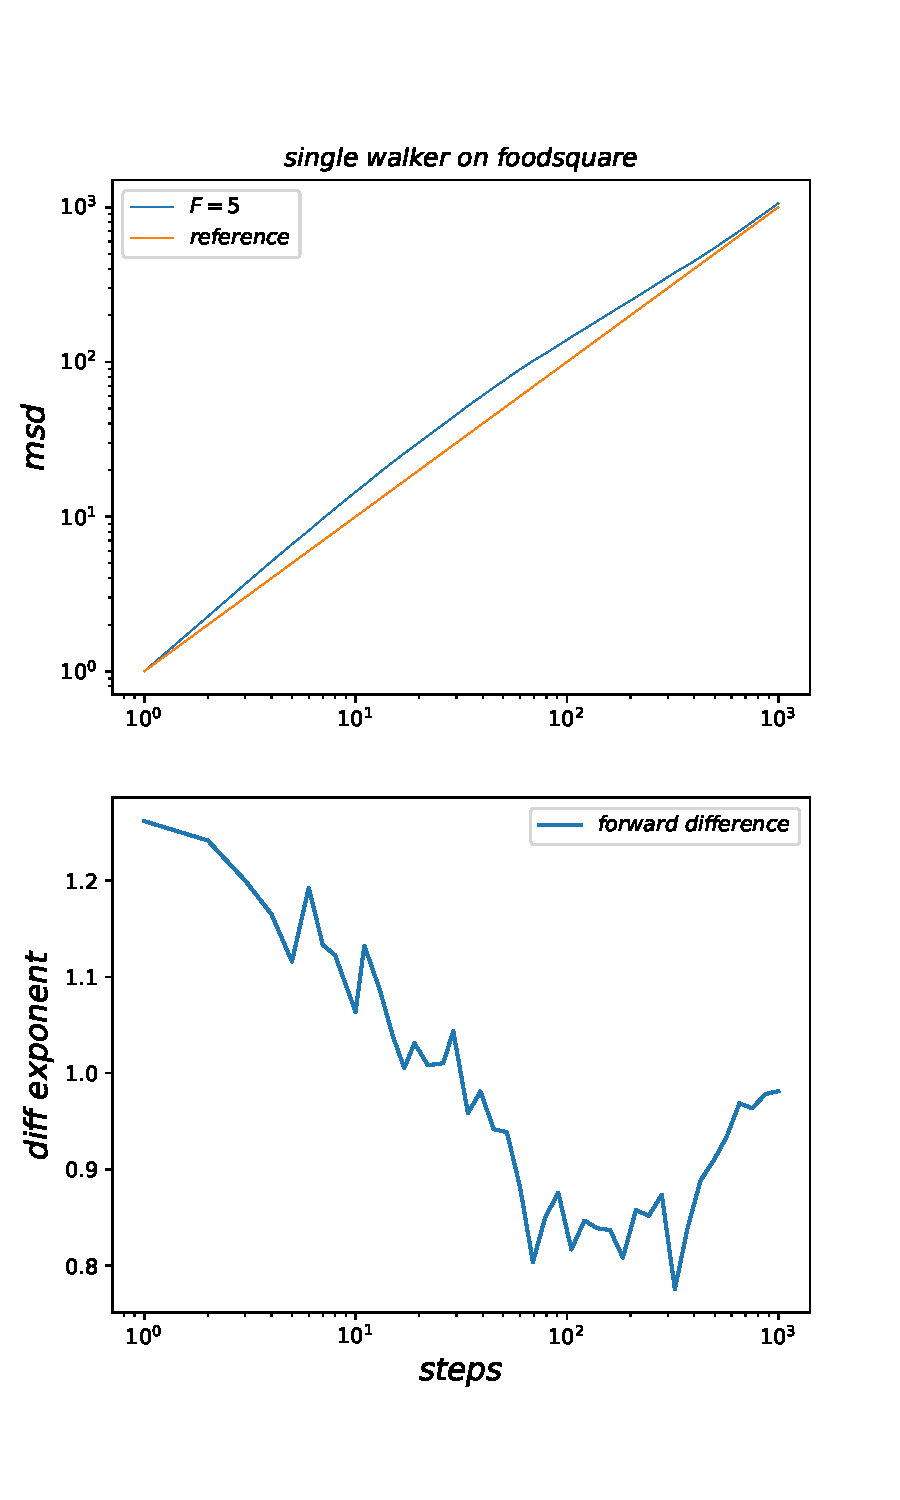
\includegraphics[scale=0.75]{300shifted_single_walker_on20x20.pdf}
	\caption{Ergebniss der MC-Simulation des oben vorgestellten Minimalmodells, mit um 300 Schritte verschobenem Aufpunkt. Es wurde über $10^5$ Samples gemittelt.}
\end{figure}


\noindent Nachfolgende Abbildungen zeigen, dass der Effekt sich (zeitlich) verschieben lässt, wenn das Nahrungsquadrat eine andere Größe besitzt. In jedem Fall ist es klar zu sehen, dass zum Zeitpunkt des Wechsels zwischen Superdiffusion nach strenger/echter Subdiffusion der Abstand zum Rand der Nahrung etwa mit der Wurzel aus dem $msd$ übereinstimmt.
\\


\begin{figure}[H]
	\centering
	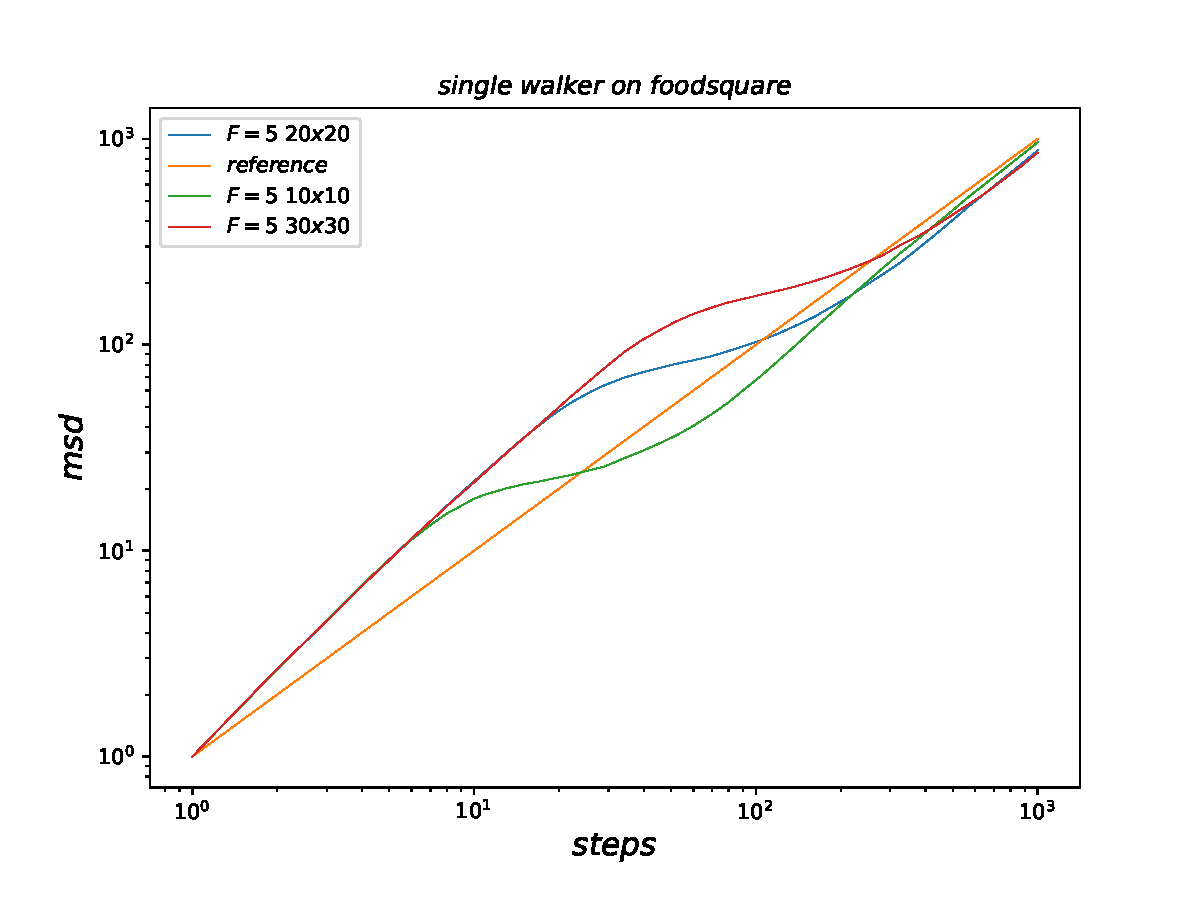
\includegraphics[scale=0.8]{abc.pdf}
	\caption{Ergebniss der MC-Simulation eines einzelnen Walkers auf Nahrungsquadraten unterschiedlicher Größe.}
\end{figure}

\clearpage

\section{PAC-MAN Verhalten als unendliche Transiente}
Die vorangegangenen Diskussionen dieses Kapitels und auch insbesondere von Kapitel 5 haben geziegt, dass die Nahrung den Prozess und auch damit das $msd$ transient macht. Dieses transiente $msd$ und insbesondere die Steigung des $msd$ im doppelt logarithmischen Plot waren sehr mit Vorsicht zu analysieren. 
\\
Meistens werden $msd$'s von nicht transienten Prozessen im Gleichgewicht betrachtet, wie zum Beispiel der klassische Random-Walk oder der Random-Walk auf dem perkolierenden Cluster \cite{PhysRevLett.50.77}, hier lassen sich aus dem $msd$ und der Steigung des $msd$ im doppelt logarithmischen Plot klare Aussagen über die Ausbreitung der Teilchen (beziehungsweise Walker) treffen. Bei transienten Prozessen ist dem nicht so.In Kapitel 4 wurde durch Simulation gezeigt, das auch in Bereichen wo der Exponent, also die Steigung des $msd$ im doppelt logarithmischen Plot kleiner als 1 ist, aber die Walker sich trotzdem stärker als diffusiv ausbreiten. In dem Limes langer Zeiten $t \rightarrow \infty$ muss sich jedes mal durch das Verschwinden der Nahrung Diffusion einstellen und zu Beginn muss durch die Nahrung, durch welche zuvor unbesuchte Felder bevorzugt werden, der Prozess superdiffusiv (also bei mittleren Dichten, wo sich die Walker ein paar Schritte zumindest gegenseitig nicht spüren) ablaufen. Es ergibt sich also aus diesen beiden Grundlagen schon automatisch, dass es einen mittleren Zeitabschnitt mit einer Steigung kleiner als 1 im $msd$ geben muss, wobei aber zunächst die wahre Dynamik/Ausbreitung hier nicht offensichtlich ist. Dieser Zeitbereich war von dem Nahrungsvorrat und damit der Walkerdichte abhängig.
\\
In Kapitel 5 wurden ähnliche Resultate gefunden, auch hier konnte man finden, dass die Walker auf lange Zeiten, je nach der Dichte, auf der Referenzkurve $F=0$ also der des Random-Walk auf dem perkolierenden Clusters (siehe oben) liegen müssen. Wohingegen erneut die Dynamik auf kurzen Zeiten ungefähr derer des Self-Avoiding Walks entsprechen muss (für große $F$ wie $F=5$ zumindest), siehe Abbildung \ref{food_thomas} aus \cite{doi:10.1063/1.4999485}. Es gibt sich also wieder eine mittlere Zeitskala welche eine Steigung kleiner als diejenige der Referenzkurve $F=0$ haben muss. In Kapitel 5 wurde herausgefunden, das diese Zeitskala durch verringern der Dichte nach hinten geschoben werden kann. In dem Paper \cite{doi:10.1063/1.4999485} wird mit einem 'hash-table' gearbeitet. Es existiert also nur ein einziger Walker und keine periodischen Kopien, in den periodischen Kopien der Simulationsbox, die Dichte ist dementsprechend 0. Man kann also den neu gefunden Exponenten der PAC-MAN Dynamik auf als eine unendliche Transiente auffassen.



\chapter{Nachfüllen der Nahrung}

\section{Einleitung/Idee}

Die vorangegangen Kapitel haben (numerisch) gezeigt, dass $msd$'s des PAC-MAN Prozesses und seiner weiteren Varianten transient sind. Dieses transiente Verhalten wird durch das 'leerfressen' der Nahrung verursacht. Man kann also für Dichten $\rho > 0$ nur eine dauerhafte Dynamik erhalten (quasi eine unendlich lange Transiente, wie in \cite{doi:10.1063/1.4999485}), in dem man künstlich, also durch zufälliges nachfüllen, einen annähernd konstanten Nahrungsvorrat schafft.
\\
Hier wird die offensichtliche Variante gewählt, dass für jeden Walker in der Simulationsbox, nach jedem Schritt einmal versucht wird eine neue Nahrungseinheit $F$ zu platzieren. Dazu wird nach jedem Schritt pro Walker eine zufällige Position (auf dem perkolierenden Cluster natürlich) gewählt und, falls keine Nahrungseinheit vorhanden ist, mit Nahrung aufgefüllt. So wird sich je nach Walkerdichte immer ein gewisser Nahrungsvorrat einstellen. Denn ist die Nahrungsmatrix schon stark geleert so werden viele Auffüllversuche akzeptiert, bei hingegen stark gefüllter Nahrungsmatrix werden die Auffüllveruche mit hoher Wahrscheinlichkeit abgelehnt. Dies entspricht also einer Art konstantes chemisches Potential Simulation für die Nahrung.
\\
Wichtig ist zu erwähnen, das nicht zu viele Auffüllversuche unternommen werden sollten, da es schlecht ist, wenn man quasi immer die gerade 'leergefressenen' Felder wieder befüllt, denn so sind immer wieder alle Felder befüllt und man hat den $F=0$ Fall, denn keine Felder werden mehr anderen gegenüber bevorzugt.
\\
In diesem Kapitel soll diese Simulation, erneut mit dem gleichzeitigen Zug\-algorithmus, für mehrere Walkerdichten durchgeführt werden. Interessant sind speziell der sich einstellende Nahrungsanteil, denn dieser lässt Rückschlüsse darauf zu, wieviel Nahrung sich die Walker gegenseitig 'wegfressen' (beziehungsweise wie die Anzahl der 'neu besuchten' Gitterplätze von der Dichte abhängt).

\section{Simulation bei verschiedenen Walkerdichten}

In diesem Abschnitt werden die Simulationsergebnisse für $\rho = 10\%$ und $\rho=1\%$ vorgestellt , diskutiert und verglichen.

\subsection{10\% Walkerdichte}

In der Nachfolgenden Abbildung sind die Simulatonsergebnisse von 100 Läufen auf 10 $L=100$ Simulationsboxen bei einer Walkerdichte von 10 \% zu sehen, es wurde also über ungefähr $3\cdot 10^5$ Realisierungen gemittelt (das $msd$). Es wurden 1000 Schritte simuliert. Die Narungspropensität ist $F=5$.
\\
\\
Es ergibt sich ein transientes (da sich das Nahrungslevel noch einstellen muss und der Prozess in dieser Zeit transient ist) $msd$ zwischen der ein PAC-MAN Kurve aus \cite{doi:10.1063/1.4999485} und der Dynamik ohne Nahrung aus \cite{PhysRevLett.50.77}.
\\
Diese Dynamik ist insofern einleuchtend, da der Nahrungsvorrat ungefähr auf 52\% gehalten wird, somitgibt es immer wieder Bereiche (zeitlich sowie räumlich) in denen sich Walker nach der ein PAC-MAN Dynamik verhalten als auch andere in denen sich Walker nach der $F=0$ Dynamik verhalten.
\\
Wie zuvor erwähnt stellt sich der Nahrungsvorrat bei ungefähr 52\% ein. Bei diesem Wert werden also Ungefähr genau soviele neue Gitterplätze besucht (also Nahrungseinheiten gefressen) wie eingefügt werden. Es ist interessant zu sehen wie dieser Wert im Vergleich zu anderen Walkerdichten ist. Dieser Wert stellt sich nach grob 30 Schritten ein, ohne die Auffüllversuche ist zu diesem Zeitpunkt schon der Nahrrungsvorrat auf unter 20\%. 
\\
\\
Der ab Schritt 40 gemittelte (doppelte) Diffusionsexponent beträgt $2\nu = 0.672$ mit einer Varianz von $\sigma^2 \approx 0.001$ was leicht oberhalb von dem $F=5$ Wert aus \cite{doi:10.1063/1.4999485} und meiner eigenen Simulation mit einem Walker (aber peiodischen Kopien, welche aber auf diesen Zeitskalen noch keinen Einfluss haben). Dieser Wert ist mit 'average' (in Grün) ebenfalls in der Graphik enthalten.

\begin{figure}[H]
	\centering
	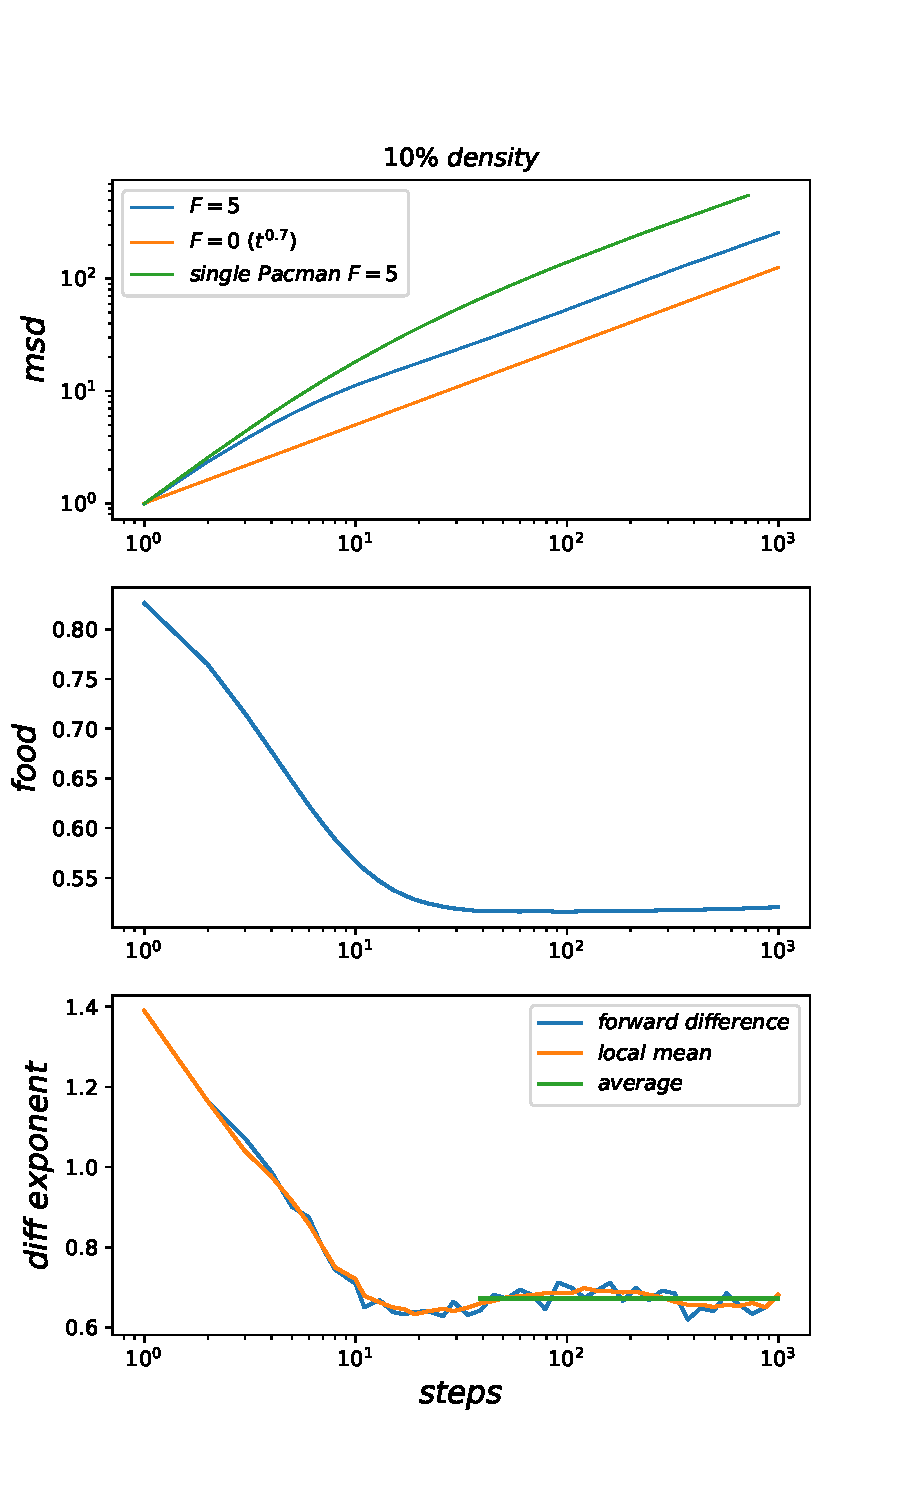
\includegraphics[scale=0.75]{10percent_new_food1.pdf}
	\caption{Ergebniss der MC-Simulation von 10\% Walkerdichte auf dem perkolierenden Cluster mit einem Auffüllversuch pro Walker und Zeitschritt.}
\end{figure}

\clearpage

\noindent Dies war aber erneut das transiente $msd$, da der Prozess nicht 'equilibriert' war, also bei (nahezu) konstantem Nahrungslevel ablief. Nun soll ebenfalls das stationäre $msd$ vorgestellt werden, dazu wird der Aufpunkt um 100 Schritte verschoben. Nach diesen 100 Schritten ist das Nahrungslevel (nahezu) konstant, man kann also sagen, dass das System 'equilibriert' ist.
\\
Man erhält nun ein deutlich 'schnelleren' Diffusionsexponenten von  $\sigma^2 \approx 0.001$ mit einer Varianz von  $\sigma^2 \approx 0.001$. Da dies ein stationäres $msd$ ist, kann man einen cross-over mit dem PAC-MAN Prozess ($2\nu \approx 0.66$) erwarten, welcher ebenfalls quasi stationär (bei Dichte $\rho=0$) bzw. unendlich lang transient ist, da der Nahrungsvorrat unendlich groß ist.

\begin{figure}[H]
	\centering
	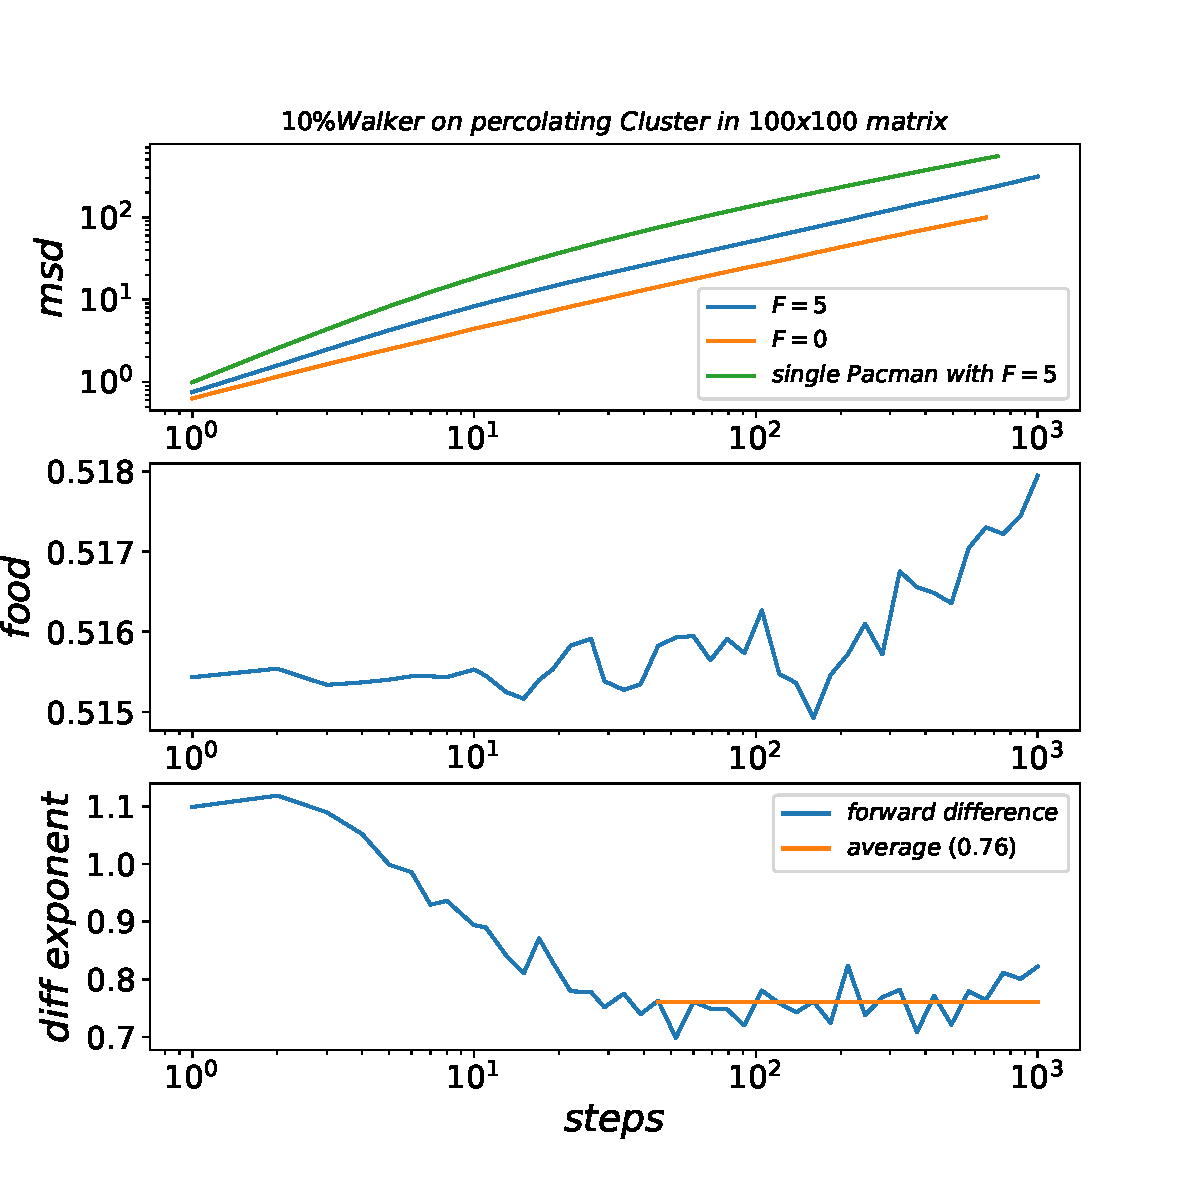
\includegraphics[scale=0.75]{new_food10_shifted100.pdf}
	\caption{Ergebniss der equilibrierten MC-Simulation (100 Schritte equilibriert) von 10\% Walkerdichte auf dem perkolierenden Cluster mit einem Auffüllversuch pro Walker und Zeitschritt.}
\end{figure}
\clearpage

\subsection{1\% Walkerdichte}

In diesem Unterabschnitt werden die Simulationsergebnisse von 200 Läufen auf 10 Matrizen der Größe $L=100$ vorgestellt. Im Gegensatz zu dem vorangegangenen Unterabschnitt liegt die Walkerdichte bei 1\% und es werden 10000 Schritte simuliert. Damit ergibt sich eine Mitteulung über etwa $2\cdot 10^4$ Realisierungen für das $msd$ und den Diffusionsexponenten.
\\
\\
Wie aus den Ergebnissen bei 10\% Walkerdichte zu erwarten war, ergibt sich erneut ein (undendlich langes) transientes $msd$ zwischen der ein PAC-MAN Kurve aus \cite{doi:10.1063/1.4999485} und der Dynamik ohne Nahrung aus \cite{PhysRevLett.50.77}. Nur ist es in diesem Fall deutlich nächer an der ein PAC-MAN Kurve, welche ja den Fall $\rho \rightarrow 0$ widerspiegelt, wobei nicht aufgefüllt wird. Wobei im Fall eines einzigen Walkers in einem unendlich großen perkolierenden Clusters, die Auffüllrate nach $0$ geht, da nur endlich viele Felder (aus unendlich vielen) keine Nahrung enthalten.
\\
Die Nahrung stellt sich oberhalb von 75\% ein und scheint etwas stärker als im Fall von 10\% Walkerdichte zu schwanken. Die Schwankungen lassen sich daran erklären, das weniger Auffüllversuche unternommen werden und so die Anzahl der angenommenen Auffüllversuche stärker schwankt.
\\
\\
Erneut kann man einen Diffusionsexponenten während der annähernd konstanten Nahrung bestimmen, dazu mittel ich die Diffusionsexponenten ab dem 495. Schritt (dieser Speicherpunkt liegt auf meinem logarithmischen Grid) und erhält einen Mittelwert von $2\nu = 0.607$ bei einer Varianz von $\sigma^2 \approx 0.01 $.

\begin{figure}[H]
	\centering
	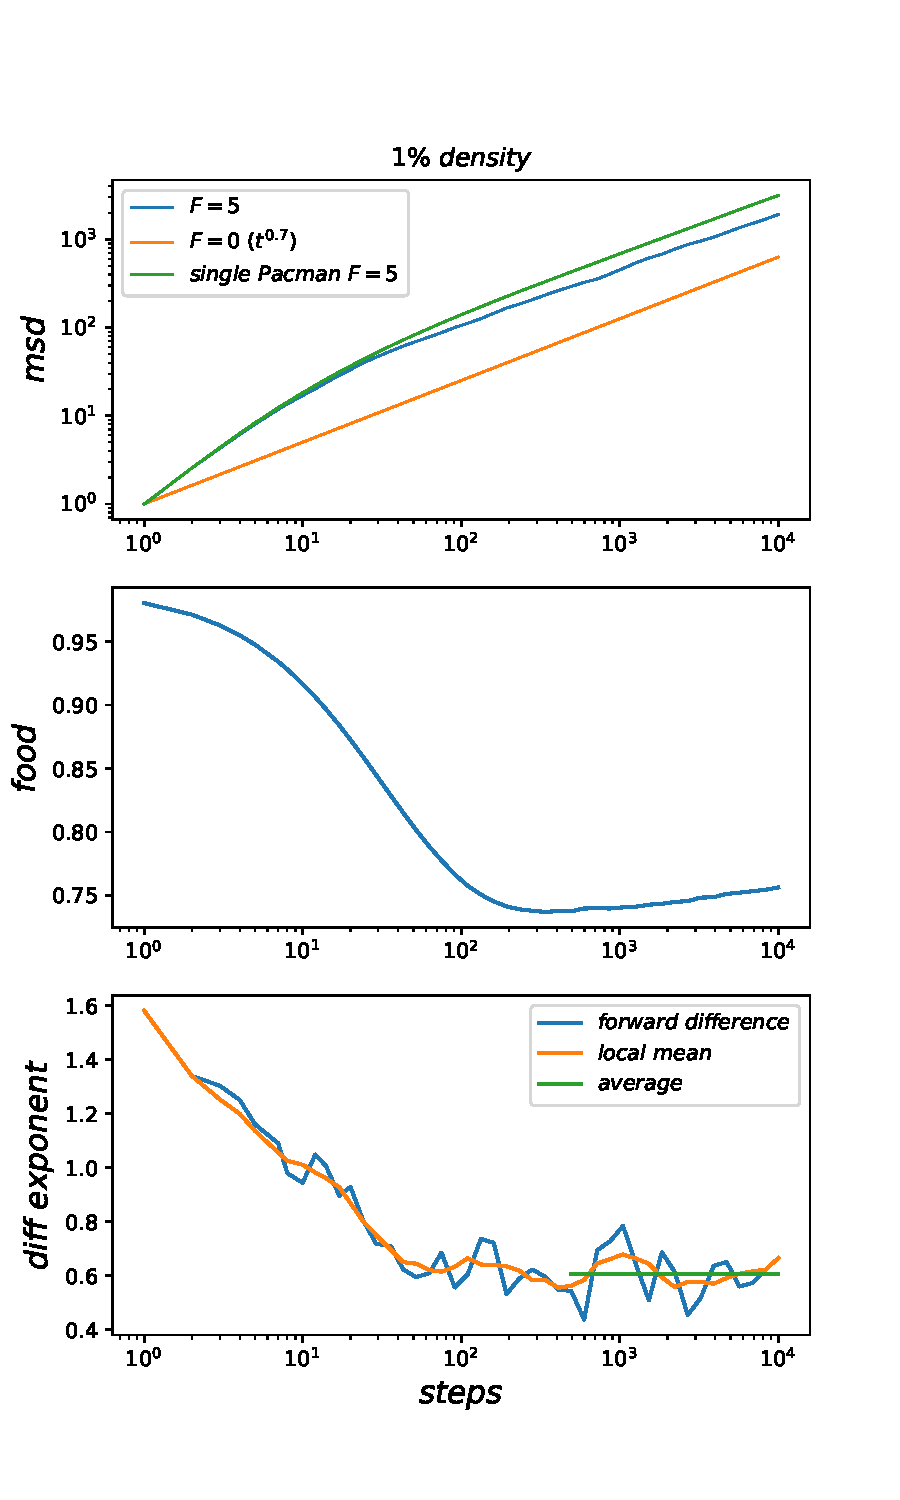
\includegraphics[scale=0.75]{1percent_new_food1.pdf}
	\caption{Ergebniss der MC-Simulation von 1\% Walkerdichte auf dem perkolierenden Cluster mit einem Auffüllversuch pro Walker und Zeitschritt.}
\end{figure}

\clearpage

\subsection{Vergleich}

Aus dem Vergleich der Vergleich der beiden Simulationenmit 10\% und 1\% Walkerdichte haben wir gesehen, dass sich bei 1\% Walkerdichte ein wesentlich höherer Nahrungsvorrat einstellt und das $msd$ auch (dementsprechend?) näher an dem eines einzelnen Walkers (Dichte $\rho \rightarrow 0$) ist. Die Frage ist nun, ob ein dichteres System (also zum Beispiel wieder die 10\%) auf welchen, zum Beispiel durch mehr Auffüllversuche der Nahrungsvorrat höher gehalten wird auch näher an das $msd$ der PAC-MAN Simulation (also \cite{doi:10.1063/1.4999485}) kommt.
\\
So könnte man zeigen, dass die Interaktion über das 'wegfressen der Nahrungseinheiten', durch das auffüllen verringert wird.
\\
\\
Auch die Einstellung des Nahrungsvorrats im Bezug auf die Walkerdichte möchte ich in diesem Unterabschnitt darstellen. Dazu wurden Simulationen bei 0.5\%, 1\%, 2\%, 3\%, 4\%, 5\%, 6\%, 8\%, 10\%, 15\% und 20\% durchgeführt und ihre sich einstellenden Nahrungsniveaus (foodlevels) durch einen Polygonenzug verbunden.

\begin{figure}[H]
	\centering
	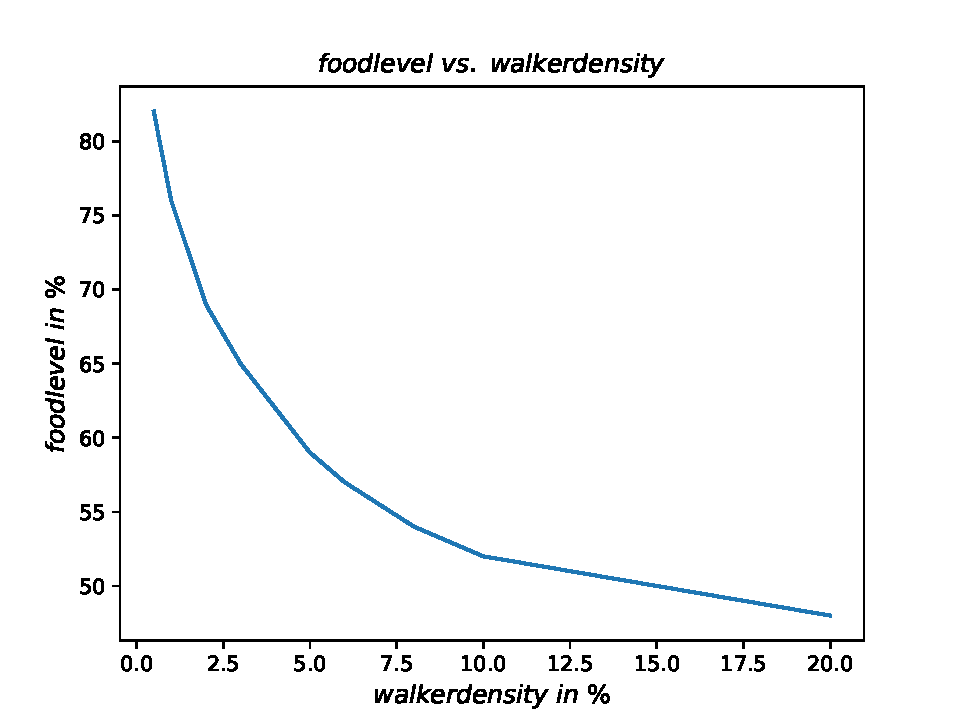
\includegraphics[scale=0.75]{flevel_vs_dens.pdf}
	\caption{Das sich einstellende Nahrungslevel in Porzent gegen die Walkerdichte in Prozent aufgetragen, bei einem Auffüllversuch pro Walker.}
\end{figure}

\clearpage

\section{Mehrere Auffüllversuche pro Walker}
In diesem Kapitel soll untersucht werden, in wie weit, das Nahrungslevel den dominanten Einfluss auf das $msd$ hat. Konkret soll bei einer Dichte $\rho$ durch mehrere (zwei oder drei) Auffüllversuche ein höheres Nahrungslevel geschaffen werden, wie es sich mit einem Auffülversuch pro Walker zu einer Dichte $\hat{\rho}<\rho$ ergibt.

\chapter{Zusammenfassung/Ausblick}
In dieser Arbeit wurden diverse Varianten des Random-Walks mit Nahrung simuliert. Der 'klassische' PAC-MAN Prozess aus \cite{doi:10.1063/1.4999485} wurde vorgestellt und erweitert auf viele, indirekt wechselwirkende, Walker, auf der freien Ebene sowie auf dem perkolierenden Cluster.
\\
Zuerst wurde versucht den 1D Random-Walk mit Nahrung analytisch zu lösen und eine vollständige Wahrscheinlichkeitsverteilung anzugeben. Hierbei wurde der 1D Walk mit Nahrung zur rechten Seite in einen Markov-Prozess eingebettet, in diesem gehört auch die Nahrungsfront zum Zustand. Es wurde die Mastergleichung aufgestellt und versucht diese in einen Kontinuumlimes zu einer partiellen Differentialgleichung zu überführen. Hierbei hat sichschon das Problem ergeben, dass zwischen der Wahrscheinlichkeit $p_{i,i}$ (Walker an Gitterplatz $i$ und Nahrungsfront auch an Gitterplatz $i$) und $p_i$ (Walker an Gitterplatz $i$ und Nahrungsfront an Gitterplatz $r \geq i$) unterschieden werden muss (siehe $p$ und $\hat{p}$). Zudem musste auch die Diskretisierung für die beiden Limits $F=0$ und $F=\infty$ unterschiedlich gewählt werden. Bei einer Wahl ergab sich im deterministischen $F=\infty$ Fall ein diffusiver Term (ähnlich wie bei der Lax-Stabilisation des 'FTCS'-Schemas). Ebenfalls konnte ich eine Kombinatorische Formel herausarbeiten welche den Fall $i=r$ (oder auch $x=r$ genannt) löst und diese für ein paar Beispiele anhand der Methode der Übergangsmatrix (von diskreten Markov-Prozessen) unterlegen (siehe dazu auch das Mathematica Notebook im Anhang).
\\
Es wurde festgestellt, dass die vielen Walker auf der freien Ebene (2D) sich durch das gegenseitige 'Wegfressen' gleichmäßiger auf dem Gitter verteilen (siehe §\ref{Dichteautokorr}).
\\
Die Simulationen mit vielen Walkern (unendlich vielen, Dichte $\rho > 0$) haben eine gewisse Skepsis an den $msd$'s und die dazu vermuteten Potenzgesetze (engl. 'power-law') und zugehörigen Diffusionsexponenten hervorgebracht. Lokale Exponenten von transienten $msd$'s zeigen nicht immer zwingend (wie zu stationären $msd$'s) die 'wahre' Ausbreitungsgeschwindigkeit der Teilchen/Walker. Der lokale Exponent bei dem Prozess mit Nahrung auf der freien Ebene hat ein subdiffusives Regime nahegelegt, welches durch eine verschobene Aufpunktswahl widerlegt werden konnte, die 'wahre' Ausbreitung war sogar stärker als diffusiv.
\\
Solche transienten $msd$'s finden sich auch in anderen Simulationen der Physik weicher Materie wie zum Beispiel in dem Paper von Zausch et al. \cite{Zausch_2008}, in dem die Dynamik kolloidaler Flüssigkeiten unter Scherung untersucht wird. Auch dort wird unter fortlaufender Scherung (transient) ab einem gewissen Punkt eine superdiffusive Dynamik beobachtet.


\appendix
\chapter{Mathematica Notebook zum 1D Walk}
In diesem Anhang möchte ich ein Mathematica Notebook vorstellen, welches die Implementation der In Kapitel 3 beschriebenen Matrixmethode zeigt. Zudem hat mir dieses Notebook geholfen meine kombinatorische $r=x$ Formel zu verifizieren.
	
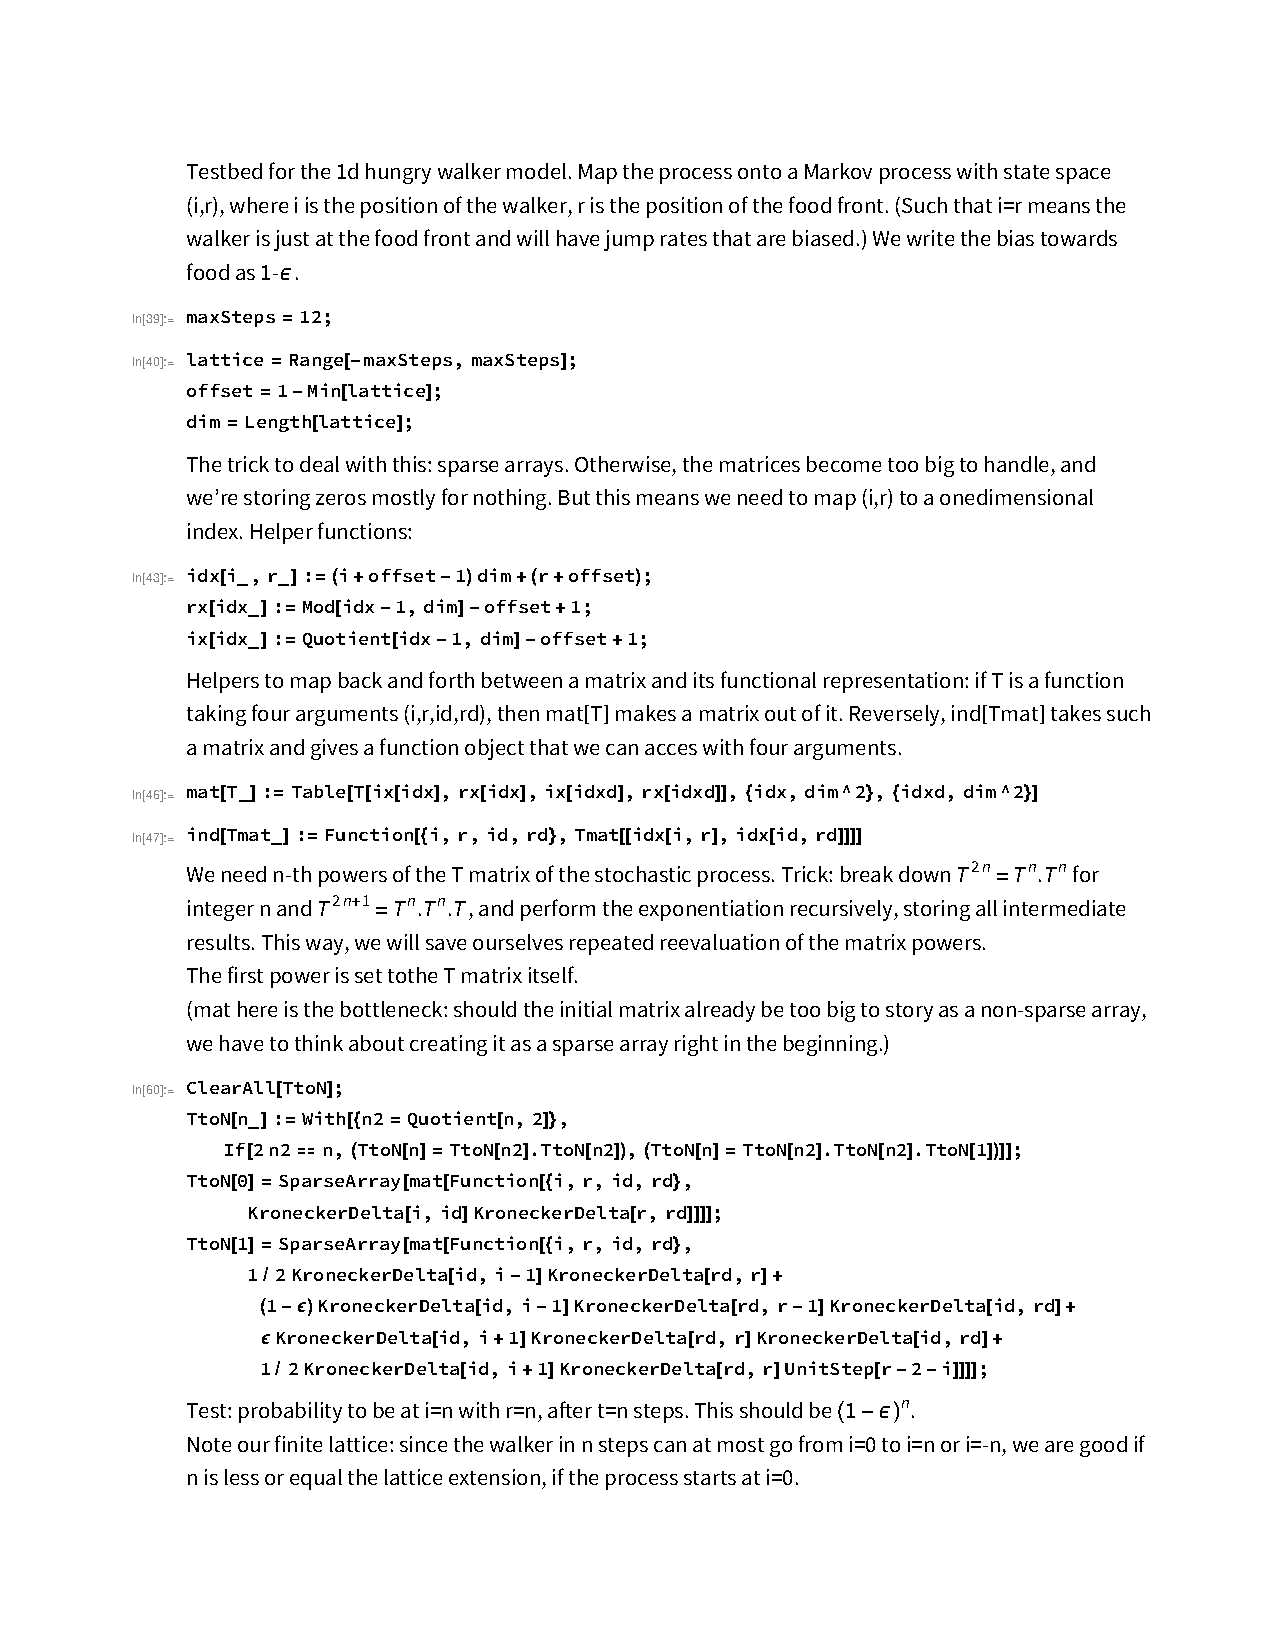
\includepdf[pages=1-2, scale=0.8]{foodwalker1d.pdf}


\bibliographystyle{plain}
\bibliography{references.bib}

\end{document}